%
% header.tex
%
\documentclass[%
	pdftex,%              PDFTex verwenden
	a4paper,%             A4 Papier
	twoside,%             Einseitig
	bibtotoc,%    Literaturverzeichnis nummeriert einf�gen
	idxtotoc,%            Index ins Verzeichnis einf�gen
	halfparskip,%         Europ�ischer Satz mit abstand zwischen Abs�tzen
	chapterprefix,%       Kapitel anschreiben als Kapitel
	headsepline,%         Linie nach Kopfzeile
	%footsepline,%         Linie vor Fusszeile
	12pt,%                 Gr�ssere Schrift, besser lesbar am bildschrim
	openright,
	pointlessnumbers
]{scrbook}

\usepackage{scrpage2}

\usepackage{textcomp}

\newcommand{\xirp}{$\chi$irp\index{xirp@$\chi$irp}}
\newcommand{\xirpname}{\enquote{eXtendable interface for robotic purposes}}
\newcommand{\version}{2.4.0}
\newcommand{\devguideurl}{http://developer.berlios.de/docman/display_doc.php?docid=1711&group_id=8442}
\newcommand{\devguideurlname}{xirp.berlios.de}
\newcommand{\seegls}[1]{\textuparrow{#1}}

\usepackage{scrpage2}

% \renewcommand{\partformat}{\partname~\thepart}
% \renewcommand{\chapterformat}{\chapapp~\thechapter}
% \renewcommand{\othersectionlevelsformat}[1]{\csname the#1\endcsname\enskip}
% 
% \renewcommand{\partmarkformat}{\thepart\enskip}
% \renewcommand{\chaptermarkformat}{\chapapp~\thechapter\enskip}
% \renewcommand{\sectionmarkformat}{\thesection\enskip}
% \renewcommand{\subsectionmarkformat}{\thesubsection\enskip}
% \renewcommand{\subsubsectionmarkformat}{\thesubsubsection\enskip}
% \renewcommand{\paragraphmarkformat}{\theparagraph\enskip}
% \renewcommand{\subparagraphmarkformat}{\thesubparagraphmarkformat\enskip}

\renewcommand{\chaptermark}[1]{\markboth{\chaptermarkformat{#1}}{\chaptermarkformat{#1}}}

\renewcommand{\chapterpagestyle}{scrheadings}
\renewcommand{\indexpagestyle}{scrheadings}

% kopf und fusszeilen
\pagestyle{scrheadings}

\clearscrheadfoot
\rohead[\headmark~\pagemark]{\headmark~\pagemark}
\lehead[\pagemark~\headmark]{\pagemark~\headmark}
\setheadtopline{.4pt}
\setheadsepline{.4pt}

\setcounter{secnumdepth}{5}
\setcounter{tocdepth}{5}

% Paket f�r die Indexerstellung.
\usepackage{makeidx}
%Formattierungen f�r Indexfile
%Erste Ebene
\newcommand*{\indexdelim}{\ \hspace{0pt plus 1fil}\penalty0\null\nobreak
  \dotfill~}
%Zweite Ebene
\newcommand*{\indexdelimi}{~\dotfill\penalty0\ }
%Dritte Ebene
\newcommand*{\indexdelimii}{~\dotfill\penalty0\ }

%Abschnitts�berschrift
\newcommand*{\indexsection}[1]{%
  \ifx\empty#1\empty\else
  \hspace{0pt plus 2fil}{{\usekomafont{sectioning} #1}}\hspace{0pt plus
    1fil}\nopagebreak
  \fi
}
% Paket f�r �bersetzungen ins Deutsche
\usepackage[french,ngerman]{babel}

% Pakete um Latin1 Zeichnens�tze verwenden zu k�nnen und die dazu
% passenden Schriften.
\usepackage[latin1]{inputenc}
\usepackage[T1]{fontenc}

% Paket f�r Quotes
\usepackage[babel,french=guillemets,german=swiss]{csquotes}

% Paket um die Symbole des TS1 Zeichensatzes verwenden zu k�nnen.
%\usepackage{textcomp}

% Paket zum Erweitern der Tabelleneigenschaften
\usepackage{array}

% Paket um Grafiken einbetten zu k�nnen
\usepackage[pdftex]{graphicx}

% Spezielle Schrift verwenden.
%\usepackage{goudysans}

% Spezielle Schrift im Koma-Script setzen.
%\setkomafont{sectioning}{\normalfont\bfseries}
%\setkomafont{captionlabel}{\normalfont\bfseries}
%\setkomafont{pagehead}{\normalfont\itshape}
%\setkomafont{descriptionlabel}{\normalfont\bfseries}

% Zeilenumbruch bei Bildbeschreibungen.
\setcapindent{1em}

% mathematische symbole aus dem AMS Paket.
%\usepackage{amsmath}
%\usepackage{amssymb}

% Type 1 Fonts f�r bessere darstellung in PDF verwenden.
%\usepackage{mathptmx}           % Times + passende Mathefonts
%\usepackage[scaled=.92]{helvet} % skalierte Helvetica als \sfdefault
%\usepackage{courier}            % Courier als \ttdefault

% Paket um Textteile drehen zu k�nnen
\usepackage{rotating}

% Package f�r Farben im PDF
\usepackage{color}
\definecolor{AliceBlue}{rgb}{0.94,0.97,1.00}
\definecolor{AntiqueWhite1}{rgb}{1.00,0.94,0.86}
\definecolor{AntiqueWhite2}{rgb}{0.93,0.87,0.80}
\definecolor{AntiqueWhite3}{rgb}{0.80,0.75,0.69}
\definecolor{AntiqueWhite4}{rgb}{0.55,0.51,0.47}
\definecolor{AntiqueWhite}{rgb}{0.98,0.92,0.84}
\definecolor{BlanchedAlmond}{rgb}{1.00,0.92,0.80}
\definecolor{BlueViolet}{rgb}{0.54,0.17,0.89}
\definecolor{CadetBlue1}{rgb}{0.60,0.96,1.00}
\definecolor{CadetBlue2}{rgb}{0.56,0.90,0.93}
\definecolor{CadetBlue3}{rgb}{0.48,0.77,0.80}
\definecolor{CadetBlue4}{rgb}{0.33,0.53,0.55}
\definecolor{CadetBlue}{rgb}{0.37,0.62,0.63}
\definecolor{CornflowerBlue}{rgb}{0.39,0.58,0.93}
\definecolor{DarkBlue}{rgb}{0.00,0.00,0.55}
\definecolor{DarkCyan}{rgb}{0.00,0.55,0.55}
\definecolor{DarkGoldenrod1}{rgb}{1.00,0.73,0.06}
\definecolor{DarkGoldenrod2}{rgb}{0.93,0.68,0.05}
\definecolor{DarkGoldenrod3}{rgb}{0.80,0.58,0.05}
\definecolor{DarkGoldenrod4}{rgb}{0.55,0.40,0.03}
\definecolor{DarkGoldenrod}{rgb}{0.72,0.53,0.04}
\definecolor{DarkGray}{rgb}{0.66,0.66,0.66}
\definecolor{DarkGreen}{rgb}{0.00,0.39,0.00}
\definecolor{DarkGrey}{rgb}{0.66,0.66,0.66}
\definecolor{DarkKhaki}{rgb}{0.74,0.72,0.42}
\definecolor{DarkMagenta}{rgb}{0.55,0.00,0.55}
\definecolor{DarkOliveGreen1}{rgb}{0.79,1.00,0.44}
\definecolor{DarkOliveGreen2}{rgb}{0.74,0.93,0.41}
\definecolor{DarkOliveGreen3}{rgb}{0.64,0.80,0.35}
\definecolor{DarkOliveGreen4}{rgb}{0.43,0.55,0.24}
\definecolor{DarkOliveGreen}{rgb}{0.33,0.42,0.18}
\definecolor{DarkOrange1}{rgb}{1.00,0.50,0.00}
\definecolor{DarkOrange2}{rgb}{0.93,0.46,0.00}
\definecolor{DarkOrange3}{rgb}{0.80,0.40,0.00}
\definecolor{DarkOrange4}{rgb}{0.55,0.27,0.00}
\definecolor{DarkOrange}{rgb}{1.00,0.55,0.00}
\definecolor{DarkOrchid1}{rgb}{0.75,0.24,1.00}
\definecolor{DarkOrchid2}{rgb}{0.70,0.23,0.93}
\definecolor{DarkOrchid3}{rgb}{0.60,0.20,0.80}
\definecolor{DarkOrchid4}{rgb}{0.41,0.13,0.55}
\definecolor{DarkOrchid}{rgb}{0.60,0.20,0.80}
\definecolor{DarkRed}{rgb}{0.55,0.00,0.00}
\definecolor{DarkSalmon}{rgb}{0.91,0.59,0.48}
\definecolor{DarkSeaGreen1}{rgb}{0.76,1.00,0.76}
\definecolor{DarkSeaGreen2}{rgb}{0.71,0.93,0.71}
\definecolor{DarkSeaGreen3}{rgb}{0.61,0.80,0.61}
\definecolor{DarkSeaGreen4}{rgb}{0.41,0.55,0.41}
\definecolor{DarkSeaGreen}{rgb}{0.56,0.74,0.56}
\definecolor{DarkSlateBlue}{rgb}{0.28,0.24,0.55}
\definecolor{DarkSlateGray1}{rgb}{0.59,1.00,1.00}
\definecolor{DarkSlateGray2}{rgb}{0.55,0.93,0.93}
\definecolor{DarkSlateGray3}{rgb}{0.47,0.80,0.80}
\definecolor{DarkSlateGray4}{rgb}{0.32,0.55,0.55}
\definecolor{DarkSlateGray}{rgb}{0.18,0.31,0.31}
\definecolor{DarkSlateGrey}{rgb}{0.18,0.31,0.31}
\definecolor{DarkTurquoise}{rgb}{0.00,0.81,0.82}
\definecolor{DarkViolet}{rgb}{0.58,0.00,0.83}
\definecolor{DeepPink1}{rgb}{1.00,0.08,0.58}
\definecolor{DeepPink2}{rgb}{0.93,0.07,0.54}
\definecolor{DeepPink3}{rgb}{0.80,0.06,0.46}
\definecolor{DeepPink4}{rgb}{0.55,0.04,0.31}
\definecolor{DeepPink}{rgb}{1.00,0.08,0.58}
\definecolor{DeepSkyBlue1}{rgb}{0.00,0.75,1.00}
\definecolor{DeepSkyBlue2}{rgb}{0.00,0.70,0.93}
\definecolor{DeepSkyBlue3}{rgb}{0.00,0.60,0.80}
\definecolor{DeepSkyBlue4}{rgb}{0.00,0.41,0.55}
\definecolor{DeepSkyBlue}{rgb}{0.00,0.75,1.00}
\definecolor{DimGray}{rgb}{0.41,0.41,0.41}
\definecolor{DimGrey}{rgb}{0.41,0.41,0.41}
\definecolor{DodgerBlue1}{rgb}{0.12,0.56,1.00}
\definecolor{DodgerBlue2}{rgb}{0.11,0.53,0.93}
\definecolor{DodgerBlue3}{rgb}{0.09,0.45,0.80}
\definecolor{DodgerBlue4}{rgb}{0.06,0.31,0.55}
\definecolor{DodgerBlue}{rgb}{0.12,0.56,1.00}
\definecolor{FloralWhite}{rgb}{1.00,0.98,0.94}
\definecolor{ForestGreen}{rgb}{0.13,0.55,0.13}
\definecolor{GhostWhite}{rgb}{0.97,0.97,1.00}
\definecolor{GreenYellow}{rgb}{0.68,1.00,0.18}
\definecolor{HotPink1}{rgb}{1.00,0.43,0.71}
\definecolor{HotPink2}{rgb}{0.93,0.42,0.65}
\definecolor{HotPink3}{rgb}{0.80,0.38,0.56}
\definecolor{HotPink4}{rgb}{0.55,0.23,0.38}
\definecolor{HotPink}{rgb}{1.00,0.41,0.71}
\definecolor{IndianRed1}{rgb}{1.00,0.42,0.42}
\definecolor{IndianRed2}{rgb}{0.93,0.39,0.39}
\definecolor{IndianRed3}{rgb}{0.80,0.33,0.33}
\definecolor{IndianRed4}{rgb}{0.55,0.23,0.23}
\definecolor{IndianRed}{rgb}{0.80,0.36,0.36}
\definecolor{LavenderBlush1}{rgb}{1.00,0.94,0.96}
\definecolor{LavenderBlush2}{rgb}{0.93,0.88,0.90}
\definecolor{LavenderBlush3}{rgb}{0.80,0.76,0.77}
\definecolor{LavenderBlush4}{rgb}{0.55,0.51,0.53}
\definecolor{LavenderBlush}{rgb}{1.00,0.94,0.96}
\definecolor{LawnGreen}{rgb}{0.49,0.99,0.00}
\definecolor{LemonChiffon1}{rgb}{1.00,0.98,0.80}
\definecolor{LemonChiffon2}{rgb}{0.93,0.91,0.75}
\definecolor{LemonChiffon3}{rgb}{0.80,0.79,0.65}
\definecolor{LemonChiffon4}{rgb}{0.55,0.54,0.44}
\definecolor{LemonChiffon}{rgb}{1.00,0.98,0.80}
\definecolor{LightBlue1}{rgb}{0.75,0.94,1.00}
\definecolor{LightBlue2}{rgb}{0.70,0.87,0.93}
\definecolor{LightBlue3}{rgb}{0.60,0.75,0.80}
\definecolor{LightBlue4}{rgb}{0.41,0.51,0.55}
\definecolor{LightBlue}{rgb}{0.68,0.85,0.90}
\definecolor{LightCoral}{rgb}{0.94,0.50,0.50}
\definecolor{LightCyan1}{rgb}{0.88,1.00,1.00}
\definecolor{LightCyan2}{rgb}{0.82,0.93,0.93}
\definecolor{LightCyan3}{rgb}{0.71,0.80,0.80}
\definecolor{LightCyan4}{rgb}{0.48,0.55,0.55}
\definecolor{LightCyan}{rgb}{0.88,1.00,1.00}
\definecolor{LightGoldenrod1}{rgb}{1.00,0.93,0.55}
\definecolor{LightGoldenrod2}{rgb}{0.93,0.86,0.51}
\definecolor{LightGoldenrod3}{rgb}{0.80,0.75,0.44}
\definecolor{LightGoldenrod4}{rgb}{0.55,0.51,0.30}
\definecolor{LightGoldenrodYellow}{rgb}{0.98,0.98,0.82}
\definecolor{LightGoldenrod}{rgb}{0.93,0.87,0.51}
\definecolor{LightGray}{rgb}{0.83,0.83,0.83}
\definecolor{LightGreen}{rgb}{0.56,0.93,0.56}
\definecolor{LightGrey}{rgb}{0.83,0.83,0.83}
\definecolor{LightPink1}{rgb}{1.00,0.68,0.73}
\definecolor{LightPink2}{rgb}{0.93,0.64,0.68}
\definecolor{LightPink3}{rgb}{0.80,0.55,0.58}
\definecolor{LightPink4}{rgb}{0.55,0.37,0.40}
\definecolor{LightPink}{rgb}{1.00,0.71,0.76}
\definecolor{LightSalmon1}{rgb}{1.00,0.63,0.48}
\definecolor{LightSalmon2}{rgb}{0.93,0.58,0.45}
\definecolor{LightSalmon3}{rgb}{0.80,0.51,0.38}
\definecolor{LightSalmon4}{rgb}{0.55,0.34,0.26}
\definecolor{LightSalmon}{rgb}{1.00,0.63,0.48}
\definecolor{LightSeaGreen}{rgb}{0.13,0.70,0.67}
\definecolor{LightSkyBlue1}{rgb}{0.69,0.89,1.00}
\definecolor{LightSkyBlue2}{rgb}{0.64,0.83,0.93}
\definecolor{LightSkyBlue3}{rgb}{0.55,0.71,0.80}
\definecolor{LightSkyBlue4}{rgb}{0.38,0.48,0.55}
\definecolor{LightSkyBlue}{rgb}{0.53,0.81,0.98}
\definecolor{LightSlateBlue}{rgb}{0.52,0.44,1.00}
\definecolor{LightSlateGray}{rgb}{0.47,0.53,0.60}
\definecolor{LightSlateGrey}{rgb}{0.47,0.53,0.60}
\definecolor{LightSteelBlue1}{rgb}{0.79,0.88,1.00}
\definecolor{LightSteelBlue2}{rgb}{0.74,0.82,0.93}
\definecolor{LightSteelBlue3}{rgb}{0.64,0.71,0.80}
\definecolor{LightSteelBlue4}{rgb}{0.43,0.48,0.55}
\definecolor{LightSteelBlue}{rgb}{0.69,0.77,0.87}
\definecolor{LightYellow1}{rgb}{1.00,1.00,0.88}
\definecolor{LightYellow2}{rgb}{0.93,0.93,0.82}
\definecolor{LightYellow3}{rgb}{0.80,0.80,0.71}
\definecolor{LightYellow4}{rgb}{0.55,0.55,0.48}
\definecolor{LightYellow}{rgb}{1.00,1.00,0.88}
\definecolor{LimeGreen}{rgb}{0.20,0.80,0.20}
\definecolor{MediumAquamarine}{rgb}{0.40,0.80,0.67}
\definecolor{MediumBlue}{rgb}{0.00,0.00,0.80}
\definecolor{MediumOrchid1}{rgb}{0.88,0.40,1.00}
\definecolor{MediumOrchid2}{rgb}{0.82,0.37,0.93}
\definecolor{MediumOrchid3}{rgb}{0.71,0.32,0.80}
\definecolor{MediumOrchid4}{rgb}{0.48,0.22,0.55}
\definecolor{MediumOrchid}{rgb}{0.73,0.33,0.83}
\definecolor{MediumPurple1}{rgb}{0.67,0.51,1.00}
\definecolor{MediumPurple2}{rgb}{0.62,0.47,0.93}
\definecolor{MediumPurple3}{rgb}{0.54,0.41,0.80}
\definecolor{MediumPurple4}{rgb}{0.36,0.28,0.55}
\definecolor{MediumPurple}{rgb}{0.58,0.44,0.86}
\definecolor{MediumSeaGreen}{rgb}{0.24,0.70,0.44}
\definecolor{MediumSlateBlue}{rgb}{0.48,0.41,0.93}
\definecolor{MediumSpringGreen}{rgb}{0.00,0.98,0.60}
\definecolor{MediumTurquoise}{rgb}{0.28,0.82,0.80}
\definecolor{MediumVioletRed}{rgb}{0.78,0.08,0.52}
\definecolor{MidnightBlue}{rgb}{0.10,0.10,0.44}
\definecolor{MintCream}{rgb}{0.96,1.00,0.98}
\definecolor{MistyRose1}{rgb}{1.00,0.89,0.88}
\definecolor{MistyRose2}{rgb}{0.93,0.84,0.82}
\definecolor{MistyRose3}{rgb}{0.80,0.72,0.71}
\definecolor{MistyRose4}{rgb}{0.55,0.49,0.48}
\definecolor{MistyRose}{rgb}{1.00,0.89,0.88}
\definecolor{NavajoWhite1}{rgb}{1.00,0.87,0.68}
\definecolor{NavajoWhite2}{rgb}{0.93,0.81,0.63}
\definecolor{NavajoWhite3}{rgb}{0.80,0.70,0.55}
\definecolor{NavajoWhite4}{rgb}{0.55,0.47,0.37}
\definecolor{NavajoWhite}{rgb}{1.00,0.87,0.68}
\definecolor{NavyBlue}{rgb}{0.00,0.00,0.50}
\definecolor{OldLace}{rgb}{0.99,0.96,0.90}
\definecolor{OliveDrab1}{rgb}{0.75,1.00,0.24}
\definecolor{OliveDrab2}{rgb}{0.70,0.93,0.23}
\definecolor{OliveDrab3}{rgb}{0.60,0.80,0.20}
\definecolor{OliveDrab4}{rgb}{0.41,0.55,0.13}
\definecolor{OliveDrab}{rgb}{0.42,0.56,0.14}
\definecolor{OrangeRed1}{rgb}{1.00,0.27,0.00}
\definecolor{OrangeRed2}{rgb}{0.93,0.25,0.00}
\definecolor{OrangeRed3}{rgb}{0.80,0.22,0.00}
\definecolor{OrangeRed4}{rgb}{0.55,0.15,0.00}
\definecolor{OrangeRed}{rgb}{1.00,0.27,0.00}
\definecolor{PaleGoldenrod}{rgb}{0.93,0.91,0.67}
\definecolor{PaleGreen1}{rgb}{0.60,1.00,0.60}
\definecolor{PaleGreen2}{rgb}{0.56,0.93,0.56}
\definecolor{PaleGreen3}{rgb}{0.49,0.80,0.49}
\definecolor{PaleGreen4}{rgb}{0.33,0.55,0.33}
\definecolor{PaleGreen}{rgb}{0.60,0.98,0.60}
\definecolor{PaleTurquoise1}{rgb}{0.73,1.00,1.00}
\definecolor{PaleTurquoise2}{rgb}{0.68,0.93,0.93}
\definecolor{PaleTurquoise3}{rgb}{0.59,0.80,0.80}
\definecolor{PaleTurquoise4}{rgb}{0.40,0.55,0.55}
\definecolor{PaleTurquoise}{rgb}{0.69,0.93,0.93}
\definecolor{PaleVioletRed1}{rgb}{1.00,0.51,0.67}
\definecolor{PaleVioletRed2}{rgb}{0.93,0.47,0.62}
\definecolor{PaleVioletRed3}{rgb}{0.80,0.41,0.54}
\definecolor{PaleVioletRed4}{rgb}{0.55,0.28,0.36}
\definecolor{PaleVioletRed}{rgb}{0.86,0.44,0.58}
\definecolor{PapayaWhip}{rgb}{1.00,0.94,0.84}
\definecolor{PeachPuff1}{rgb}{1.00,0.85,0.73}
\definecolor{PeachPuff2}{rgb}{0.93,0.80,0.68}
\definecolor{PeachPuff3}{rgb}{0.80,0.69,0.58}
\definecolor{PeachPuff4}{rgb}{0.55,0.47,0.40}
\definecolor{PeachPuff}{rgb}{1.00,0.85,0.73}
\definecolor{PowderBlue}{rgb}{0.69,0.88,0.90}
\definecolor{RosyBrown1}{rgb}{1.00,0.76,0.76}
\definecolor{RosyBrown2}{rgb}{0.93,0.71,0.71}
\definecolor{RosyBrown3}{rgb}{0.80,0.61,0.61}
\definecolor{RosyBrown4}{rgb}{0.55,0.41,0.41}
\definecolor{RosyBrown}{rgb}{0.74,0.56,0.56}
\definecolor{RoyalBlue1}{rgb}{0.28,0.46,1.00}
\definecolor{RoyalBlue2}{rgb}{0.26,0.43,0.93}
\definecolor{RoyalBlue3}{rgb}{0.23,0.37,0.80}
\definecolor{RoyalBlue4}{rgb}{0.15,0.25,0.55}
\definecolor{RoyalBlue}{rgb}{0.25,0.41,0.88}
\definecolor{SaddleBrown}{rgb}{0.55,0.27,0.07}
\definecolor{SandyBrown}{rgb}{0.96,0.64,0.38}
\definecolor{SeaGreen1}{rgb}{0.33,1.00,0.62}
\definecolor{SeaGreen2}{rgb}{0.31,0.93,0.58}
\definecolor{SeaGreen3}{rgb}{0.26,0.80,0.50}
\definecolor{SeaGreen4}{rgb}{0.18,0.55,0.34}
\definecolor{SeaGreen}{rgb}{0.18,0.55,0.34}
\definecolor{SkyBlue1}{rgb}{0.53,0.81,1.00}
\definecolor{SkyBlue2}{rgb}{0.49,0.75,0.93}
\definecolor{SkyBlue3}{rgb}{0.42,0.65,0.80}
\definecolor{SkyBlue4}{rgb}{0.29,0.44,0.55}
\definecolor{SkyBlue}{rgb}{0.53,0.81,0.92}
\definecolor{SlateBlue1}{rgb}{0.51,0.44,1.00}
\definecolor{SlateBlue2}{rgb}{0.48,0.40,0.93}
\definecolor{SlateBlue3}{rgb}{0.41,0.35,0.80}
\definecolor{SlateBlue4}{rgb}{0.28,0.24,0.55}
\definecolor{SlateBlue}{rgb}{0.42,0.35,0.80}
\definecolor{SlateGray1}{rgb}{0.78,0.89,1.00}
\definecolor{SlateGray2}{rgb}{0.73,0.83,0.93}
\definecolor{SlateGray3}{rgb}{0.62,0.71,0.80}
\definecolor{SlateGray4}{rgb}{0.42,0.48,0.55}
\definecolor{SlateGray}{rgb}{0.44,0.50,0.56}
\definecolor{SlateGrey}{rgb}{0.44,0.50,0.56}
\definecolor{SpringGreen1}{rgb}{0.00,1.00,0.50}
\definecolor{SpringGreen2}{rgb}{0.00,0.93,0.46}
\definecolor{SpringGreen3}{rgb}{0.00,0.80,0.40}
\definecolor{SpringGreen4}{rgb}{0.00,0.55,0.27}
\definecolor{SpringGreen}{rgb}{0.00,1.00,0.50}
\definecolor{SteelBlue1}{rgb}{0.39,0.72,1.00}
\definecolor{SteelBlue2}{rgb}{0.36,0.67,0.93}
\definecolor{SteelBlue3}{rgb}{0.31,0.58,0.80}
\definecolor{SteelBlue4}{rgb}{0.21,0.39,0.55}
\definecolor{SteelBlue}{rgb}{0.27,0.51,0.71}
\definecolor{VioletRed1}{rgb}{1.00,0.24,0.59}
\definecolor{VioletRed2}{rgb}{0.93,0.23,0.55}
\definecolor{VioletRed3}{rgb}{0.80,0.20,0.47}
\definecolor{VioletRed4}{rgb}{0.55,0.13,0.32}
\definecolor{VioletRed}{rgb}{0.82,0.13,0.56}
\definecolor{WhiteSmoke}{rgb}{0.96,0.96,0.96}
\definecolor{YellowGreen}{rgb}{0.60,0.80,0.20}
\definecolor{aliceblue}{rgb}{0.94,0.97,1.00}
\definecolor{antiquewhite}{rgb}{0.98,0.92,0.84}
\definecolor{aquamarine1}{rgb}{0.50,1.00,0.83}
\definecolor{aquamarine2}{rgb}{0.46,0.93,0.78}
\definecolor{aquamarine3}{rgb}{0.40,0.80,0.67}
\definecolor{aquamarine4}{rgb}{0.27,0.55,0.45}
\definecolor{aquamarine}{rgb}{0.50,1.00,0.83}
\definecolor{azure1}{rgb}{0.94,1.00,1.00}
\definecolor{azure2}{rgb}{0.88,0.93,0.93}
\definecolor{azure3}{rgb}{0.76,0.80,0.80}
\definecolor{azure4}{rgb}{0.51,0.55,0.55}
\definecolor{azure}{rgb}{0.94,1.00,1.00}
\definecolor{beige}{rgb}{0.96,0.96,0.86}
\definecolor{bisque1}{rgb}{1.00,0.89,0.77}
\definecolor{bisque2}{rgb}{0.93,0.84,0.72}
\definecolor{bisque3}{rgb}{0.80,0.72,0.62}
\definecolor{bisque4}{rgb}{0.55,0.49,0.42}
\definecolor{bisque}{rgb}{1.00,0.89,0.77}
\definecolor{black}{rgb}{0.00,0.00,0.00}
\definecolor{blanchedalmond}{rgb}{1.00,0.92,0.80}
\definecolor{blue1}{rgb}{0.00,0.00,1.00}
\definecolor{blue2}{rgb}{0.00,0.00,0.93}
\definecolor{blue3}{rgb}{0.00,0.00,0.80}
\definecolor{blue4}{rgb}{0.00,0.00,0.55}
\definecolor{blueviolet}{rgb}{0.54,0.17,0.89}
\definecolor{blue}{rgb}{0.00,0.00,1.00}
\definecolor{brown1}{rgb}{1.00,0.25,0.25}
\definecolor{brown2}{rgb}{0.93,0.23,0.23}
\definecolor{brown3}{rgb}{0.80,0.20,0.20}
\definecolor{brown4}{rgb}{0.55,0.14,0.14}
\definecolor{brown}{rgb}{0.65,0.16,0.16}
\definecolor{burlywood1}{rgb}{1.00,0.83,0.61}
\definecolor{burlywood2}{rgb}{0.93,0.77,0.57}
\definecolor{burlywood3}{rgb}{0.80,0.67,0.49}
\definecolor{burlywood4}{rgb}{0.55,0.45,0.33}
\definecolor{burlywood}{rgb}{0.87,0.72,0.53}
\definecolor{cadetblue}{rgb}{0.37,0.62,0.63}
\definecolor{chartreuse1}{rgb}{0.50,1.00,0.00}
\definecolor{chartreuse2}{rgb}{0.46,0.93,0.00}
\definecolor{chartreuse3}{rgb}{0.40,0.80,0.00}
\definecolor{chartreuse4}{rgb}{0.27,0.55,0.00}
\definecolor{chartreuse}{rgb}{0.50,1.00,0.00}
\definecolor{chocolate1}{rgb}{1.00,0.50,0.14}
\definecolor{chocolate2}{rgb}{0.93,0.46,0.13}
\definecolor{chocolate3}{rgb}{0.80,0.40,0.11}
\definecolor{chocolate4}{rgb}{0.55,0.27,0.07}
\definecolor{chocolate}{rgb}{0.82,0.41,0.12}
\definecolor{coral1}{rgb}{1.00,0.45,0.34}
\definecolor{coral2}{rgb}{0.93,0.42,0.31}
\definecolor{coral3}{rgb}{0.80,0.36,0.27}
\definecolor{coral4}{rgb}{0.55,0.24,0.18}
\definecolor{coral}{rgb}{1.00,0.50,0.31}
\definecolor{cornflowerblue}{rgb}{0.39,0.58,0.93}
\definecolor{cornsilk1}{rgb}{1.00,0.97,0.86}
\definecolor{cornsilk2}{rgb}{0.93,0.91,0.80}
\definecolor{cornsilk3}{rgb}{0.80,0.78,0.69}
\definecolor{cornsilk4}{rgb}{0.55,0.53,0.47}
\definecolor{cornsilk}{rgb}{1.00,0.97,0.86}
\definecolor{cyan1}{rgb}{0.00,1.00,1.00}
\definecolor{cyan2}{rgb}{0.00,0.93,0.93}
\definecolor{cyan3}{rgb}{0.00,0.80,0.80}
\definecolor{cyan4}{rgb}{0.00,0.55,0.55}
\definecolor{cyan}{rgb}{0.00,1.00,1.00}
\definecolor{darkblue}{rgb}{0.00,0.00,0.55}
\definecolor{darkcyan}{rgb}{0.00,0.55,0.55}
\definecolor{darkgoldenrod}{rgb}{0.72,0.53,0.04}
\definecolor{darkgray}{rgb}{0.66,0.66,0.66}
\definecolor{darkgreen}{rgb}{0.00,0.39,0.00}
\definecolor{darkgrey}{rgb}{0.66,0.66,0.66}
\definecolor{darkkhaki}{rgb}{0.74,0.72,0.42}
\definecolor{darkmagenta}{rgb}{0.55,0.00,0.55}
\definecolor{darkolive}{rgb}{0.33,0.42,0.18}
\definecolor{darkorange}{rgb}{1.00,0.55,0.00}
\definecolor{darkorchid}{rgb}{0.60,0.20,0.80}
\definecolor{darkred}{rgb}{0.55,0.00,0.00}
\definecolor{darksalmon}{rgb}{0.91,0.59,0.48}
\definecolor{darksea}{rgb}{0.56,0.74,0.56}
\definecolor{darkslate}{rgb}{0.18,0.31,0.31}
\definecolor{darkslate}{rgb}{0.18,0.31,0.31}
\definecolor{darkslate}{rgb}{0.28,0.24,0.55}
\definecolor{darkturquoise}{rgb}{0.00,0.81,0.82}
\definecolor{darkviolet}{rgb}{0.58,0.00,0.83}
\definecolor{deeppink}{rgb}{1.00,0.08,0.58}
\definecolor{deepsky}{rgb}{0.00,0.75,1.00}
\definecolor{dimgray}{rgb}{0.41,0.41,0.41}
\definecolor{dimgrey}{rgb}{0.41,0.41,0.41}
\definecolor{dodgerblue}{rgb}{0.12,0.56,1.00}
\definecolor{firebrick1}{rgb}{1.00,0.19,0.19}
\definecolor{firebrick2}{rgb}{0.93,0.17,0.17}
\definecolor{firebrick3}{rgb}{0.80,0.15,0.15}
\definecolor{firebrick4}{rgb}{0.55,0.10,0.10}
\definecolor{firebrick}{rgb}{0.70,0.13,0.13}
\definecolor{floralwhite}{rgb}{1.00,0.98,0.94}
\definecolor{forestgreen}{rgb}{0.13,0.55,0.13}
\definecolor{gainsboro}{rgb}{0.86,0.86,0.86}
\definecolor{ghostwhite}{rgb}{0.97,0.97,1.00}
\definecolor{gold1}{rgb}{1.00,0.84,0.00}
\definecolor{gold2}{rgb}{0.93,0.79,0.00}
\definecolor{gold3}{rgb}{0.80,0.68,0.00}
\definecolor{gold4}{rgb}{0.55,0.46,0.00}
\definecolor{goldenrod1}{rgb}{1.00,0.76,0.15}
\definecolor{goldenrod2}{rgb}{0.93,0.71,0.13}
\definecolor{goldenrod3}{rgb}{0.80,0.61,0.11}
\definecolor{goldenrod4}{rgb}{0.55,0.41,0.08}
\definecolor{goldenrod}{rgb}{0.85,0.65,0.13}
\definecolor{gold}{rgb}{1.00,0.84,0.00}
\definecolor{gray0}{rgb}{0.00,0.00,0.00}
\definecolor{gray100}{rgb}{1.00,1.00,1.00}
\definecolor{gray10}{rgb}{0.10,0.10,0.10}
\definecolor{gray11}{rgb}{0.11,0.11,0.11}
\definecolor{gray12}{rgb}{0.12,0.12,0.12}
\definecolor{gray13}{rgb}{0.13,0.13,0.13}
\definecolor{gray14}{rgb}{0.14,0.14,0.14}
\definecolor{gray15}{rgb}{0.15,0.15,0.15}
\definecolor{gray16}{rgb}{0.16,0.16,0.16}
\definecolor{gray17}{rgb}{0.17,0.17,0.17}
\definecolor{gray18}{rgb}{0.18,0.18,0.18}
\definecolor{gray19}{rgb}{0.19,0.19,0.19}
\definecolor{gray1}{rgb}{0.01,0.01,0.01}
\definecolor{gray20}{rgb}{0.20,0.20,0.20}
\definecolor{gray21}{rgb}{0.21,0.21,0.21}
\definecolor{gray22}{rgb}{0.22,0.22,0.22}
\definecolor{gray23}{rgb}{0.23,0.23,0.23}
\definecolor{gray24}{rgb}{0.24,0.24,0.24}
\definecolor{gray25}{rgb}{0.25,0.25,0.25}
\definecolor{gray26}{rgb}{0.26,0.26,0.26}
\definecolor{gray27}{rgb}{0.27,0.27,0.27}
\definecolor{gray28}{rgb}{0.28,0.28,0.28}
\definecolor{gray29}{rgb}{0.29,0.29,0.29}
\definecolor{gray2}{rgb}{0.02,0.02,0.02}
\definecolor{gray30}{rgb}{0.30,0.30,0.30}
\definecolor{gray31}{rgb}{0.31,0.31,0.31}
\definecolor{gray32}{rgb}{0.32,0.32,0.32}
\definecolor{gray33}{rgb}{0.33,0.33,0.33}
\definecolor{gray34}{rgb}{0.34,0.34,0.34}
\definecolor{gray35}{rgb}{0.35,0.35,0.35}
\definecolor{gray36}{rgb}{0.36,0.36,0.36}
\definecolor{gray37}{rgb}{0.37,0.37,0.37}
\definecolor{gray38}{rgb}{0.38,0.38,0.38}
\definecolor{gray39}{rgb}{0.39,0.39,0.39}
\definecolor{gray3}{rgb}{0.03,0.03,0.03}
\definecolor{gray40}{rgb}{0.40,0.40,0.40}
\definecolor{gray41}{rgb}{0.41,0.41,0.41}
\definecolor{gray42}{rgb}{0.42,0.42,0.42}
\definecolor{gray43}{rgb}{0.43,0.43,0.43}
\definecolor{gray44}{rgb}{0.44,0.44,0.44}
\definecolor{gray45}{rgb}{0.45,0.45,0.45}
\definecolor{gray46}{rgb}{0.46,0.46,0.46}
\definecolor{gray47}{rgb}{0.47,0.47,0.47}
\definecolor{gray48}{rgb}{0.48,0.48,0.48}
\definecolor{gray49}{rgb}{0.49,0.49,0.49}
\definecolor{gray4}{rgb}{0.04,0.04,0.04}
\definecolor{gray50}{rgb}{0.50,0.50,0.50}
\definecolor{gray51}{rgb}{0.51,0.51,0.51}
\definecolor{gray52}{rgb}{0.52,0.52,0.52}
\definecolor{gray53}{rgb}{0.53,0.53,0.53}
\definecolor{gray54}{rgb}{0.54,0.54,0.54}
\definecolor{gray55}{rgb}{0.55,0.55,0.55}
\definecolor{gray56}{rgb}{0.56,0.56,0.56}
\definecolor{gray57}{rgb}{0.57,0.57,0.57}
\definecolor{gray58}{rgb}{0.58,0.58,0.58}
\definecolor{gray59}{rgb}{0.59,0.59,0.59}
\definecolor{gray5}{rgb}{0.05,0.05,0.05}
\definecolor{gray60}{rgb}{0.60,0.60,0.60}
\definecolor{gray61}{rgb}{0.61,0.61,0.61}
\definecolor{gray62}{rgb}{0.62,0.62,0.62}
\definecolor{gray63}{rgb}{0.63,0.63,0.63}
\definecolor{gray64}{rgb}{0.64,0.64,0.64}
\definecolor{gray65}{rgb}{0.65,0.65,0.65}
\definecolor{gray66}{rgb}{0.66,0.66,0.66}
\definecolor{gray67}{rgb}{0.67,0.67,0.67}
\definecolor{gray68}{rgb}{0.68,0.68,0.68}
\definecolor{gray69}{rgb}{0.69,0.69,0.69}
\definecolor{gray6}{rgb}{0.06,0.06,0.06}
\definecolor{gray70}{rgb}{0.70,0.70,0.70}
\definecolor{gray71}{rgb}{0.71,0.71,0.71}
\definecolor{gray72}{rgb}{0.72,0.72,0.72}
\definecolor{gray73}{rgb}{0.73,0.73,0.73}
\definecolor{gray74}{rgb}{0.74,0.74,0.74}
\definecolor{gray75}{rgb}{0.75,0.75,0.75}
\definecolor{gray76}{rgb}{0.76,0.76,0.76}
\definecolor{gray77}{rgb}{0.77,0.77,0.77}
\definecolor{gray78}{rgb}{0.78,0.78,0.78}
\definecolor{gray79}{rgb}{0.79,0.79,0.79}
\definecolor{gray7}{rgb}{0.07,0.07,0.07}
\definecolor{gray80}{rgb}{0.80,0.80,0.80}
\definecolor{gray81}{rgb}{0.81,0.81,0.81}
\definecolor{gray82}{rgb}{0.82,0.82,0.82}
\definecolor{gray83}{rgb}{0.83,0.83,0.83}
\definecolor{gray84}{rgb}{0.84,0.84,0.84}
\definecolor{gray85}{rgb}{0.85,0.85,0.85}
\definecolor{gray86}{rgb}{0.86,0.86,0.86}
\definecolor{gray87}{rgb}{0.87,0.87,0.87}
\definecolor{gray88}{rgb}{0.88,0.88,0.88}
\definecolor{gray89}{rgb}{0.89,0.89,0.89}
\definecolor{gray8}{rgb}{0.08,0.08,0.08}
\definecolor{gray90}{rgb}{0.90,0.90,0.90}
\definecolor{gray91}{rgb}{0.91,0.91,0.91}
\definecolor{gray92}{rgb}{0.92,0.92,0.92}
\definecolor{gray93}{rgb}{0.93,0.93,0.93}
\definecolor{gray94}{rgb}{0.94,0.94,0.94}
\definecolor{gray95}{rgb}{0.95,0.95,0.95}
\definecolor{gray96}{rgb}{0.96,0.96,0.96}
\definecolor{gray97}{rgb}{0.97,0.97,0.97}
\definecolor{gray98}{rgb}{0.98,0.98,0.98}
\definecolor{gray99}{rgb}{0.99,0.99,0.99}
\definecolor{gray9}{rgb}{0.09,0.09,0.09}
\definecolor{gray}{rgb}{0.75,0.75,0.75}
\definecolor{green1}{rgb}{0.00,1.00,0.00}
\definecolor{green2}{rgb}{0.00,0.93,0.00}
\definecolor{green3}{rgb}{0.00,0.80,0.00}
\definecolor{green4}{rgb}{0.00,0.55,0.00}
\definecolor{greenyellow}{rgb}{0.68,1.00,0.18}
\definecolor{green}{rgb}{0.00,1.00,0.00}
\definecolor{grey0}{rgb}{0.00,0.00,0.00}
\definecolor{grey100}{rgb}{1.00,1.00,1.00}
\definecolor{grey10}{rgb}{0.10,0.10,0.10}
\definecolor{grey11}{rgb}{0.11,0.11,0.11}
\definecolor{grey12}{rgb}{0.12,0.12,0.12}
\definecolor{grey13}{rgb}{0.13,0.13,0.13}
\definecolor{grey14}{rgb}{0.14,0.14,0.14}
\definecolor{grey15}{rgb}{0.15,0.15,0.15}
\definecolor{grey16}{rgb}{0.16,0.16,0.16}
\definecolor{grey17}{rgb}{0.17,0.17,0.17}
\definecolor{grey18}{rgb}{0.18,0.18,0.18}
\definecolor{grey19}{rgb}{0.19,0.19,0.19}
\definecolor{grey1}{rgb}{0.01,0.01,0.01}
\definecolor{grey20}{rgb}{0.20,0.20,0.20}
\definecolor{grey21}{rgb}{0.21,0.21,0.21}
\definecolor{grey22}{rgb}{0.22,0.22,0.22}
\definecolor{grey23}{rgb}{0.23,0.23,0.23}
\definecolor{grey24}{rgb}{0.24,0.24,0.24}
\definecolor{grey25}{rgb}{0.25,0.25,0.25}
\definecolor{grey26}{rgb}{0.26,0.26,0.26}
\definecolor{grey27}{rgb}{0.27,0.27,0.27}
\definecolor{grey28}{rgb}{0.28,0.28,0.28}
\definecolor{grey29}{rgb}{0.29,0.29,0.29}
\definecolor{grey2}{rgb}{0.02,0.02,0.02}
\definecolor{grey30}{rgb}{0.30,0.30,0.30}
\definecolor{grey31}{rgb}{0.31,0.31,0.31}
\definecolor{grey32}{rgb}{0.32,0.32,0.32}
\definecolor{grey33}{rgb}{0.33,0.33,0.33}
\definecolor{grey34}{rgb}{0.34,0.34,0.34}
\definecolor{grey35}{rgb}{0.35,0.35,0.35}
\definecolor{grey36}{rgb}{0.36,0.36,0.36}
\definecolor{grey37}{rgb}{0.37,0.37,0.37}
\definecolor{grey38}{rgb}{0.38,0.38,0.38}
\definecolor{grey39}{rgb}{0.39,0.39,0.39}
\definecolor{grey3}{rgb}{0.03,0.03,0.03}
\definecolor{grey40}{rgb}{0.40,0.40,0.40}
\definecolor{grey41}{rgb}{0.41,0.41,0.41}
\definecolor{grey42}{rgb}{0.42,0.42,0.42}
\definecolor{grey43}{rgb}{0.43,0.43,0.43}
\definecolor{grey44}{rgb}{0.44,0.44,0.44}
\definecolor{grey45}{rgb}{0.45,0.45,0.45}
\definecolor{grey46}{rgb}{0.46,0.46,0.46}
\definecolor{grey47}{rgb}{0.47,0.47,0.47}
\definecolor{grey48}{rgb}{0.48,0.48,0.48}
\definecolor{grey49}{rgb}{0.49,0.49,0.49}
\definecolor{grey4}{rgb}{0.04,0.04,0.04}
\definecolor{grey50}{rgb}{0.50,0.50,0.50}
\definecolor{grey51}{rgb}{0.51,0.51,0.51}
\definecolor{grey52}{rgb}{0.52,0.52,0.52}
\definecolor{grey53}{rgb}{0.53,0.53,0.53}
\definecolor{grey54}{rgb}{0.54,0.54,0.54}
\definecolor{grey55}{rgb}{0.55,0.55,0.55}
\definecolor{grey56}{rgb}{0.56,0.56,0.56}
\definecolor{grey57}{rgb}{0.57,0.57,0.57}
\definecolor{grey58}{rgb}{0.58,0.58,0.58}
\definecolor{grey59}{rgb}{0.59,0.59,0.59}
\definecolor{grey5}{rgb}{0.05,0.05,0.05}
\definecolor{grey60}{rgb}{0.60,0.60,0.60}
\definecolor{grey61}{rgb}{0.61,0.61,0.61}
\definecolor{grey62}{rgb}{0.62,0.62,0.62}
\definecolor{grey63}{rgb}{0.63,0.63,0.63}
\definecolor{grey64}{rgb}{0.64,0.64,0.64}
\definecolor{grey65}{rgb}{0.65,0.65,0.65}
\definecolor{grey66}{rgb}{0.66,0.66,0.66}
\definecolor{grey67}{rgb}{0.67,0.67,0.67}
\definecolor{grey68}{rgb}{0.68,0.68,0.68}
\definecolor{grey69}{rgb}{0.69,0.69,0.69}
\definecolor{grey6}{rgb}{0.06,0.06,0.06}
\definecolor{grey70}{rgb}{0.70,0.70,0.70}
\definecolor{grey71}{rgb}{0.71,0.71,0.71}
\definecolor{grey72}{rgb}{0.72,0.72,0.72}
\definecolor{grey73}{rgb}{0.73,0.73,0.73}
\definecolor{grey74}{rgb}{0.74,0.74,0.74}
\definecolor{grey75}{rgb}{0.75,0.75,0.75}
\definecolor{grey76}{rgb}{0.76,0.76,0.76}
\definecolor{grey77}{rgb}{0.77,0.77,0.77}
\definecolor{grey78}{rgb}{0.78,0.78,0.78}
\definecolor{grey79}{rgb}{0.79,0.79,0.79}
\definecolor{grey7}{rgb}{0.07,0.07,0.07}
\definecolor{grey80}{rgb}{0.80,0.80,0.80}
\definecolor{grey81}{rgb}{0.81,0.81,0.81}
\definecolor{grey82}{rgb}{0.82,0.82,0.82}
\definecolor{grey83}{rgb}{0.83,0.83,0.83}
\definecolor{grey84}{rgb}{0.84,0.84,0.84}
\definecolor{grey85}{rgb}{0.85,0.85,0.85}
\definecolor{grey86}{rgb}{0.86,0.86,0.86}
\definecolor{grey87}{rgb}{0.87,0.87,0.87}
\definecolor{grey88}{rgb}{0.88,0.88,0.88}
\definecolor{grey89}{rgb}{0.89,0.89,0.89}
\definecolor{grey8}{rgb}{0.08,0.08,0.08}
\definecolor{grey90}{rgb}{0.90,0.90,0.90}
\definecolor{grey91}{rgb}{0.91,0.91,0.91}
\definecolor{grey92}{rgb}{0.92,0.92,0.92}
\definecolor{grey93}{rgb}{0.93,0.93,0.93}
\definecolor{grey94}{rgb}{0.94,0.94,0.94}
\definecolor{grey95}{rgb}{0.95,0.95,0.95}
\definecolor{grey96}{rgb}{0.96,0.96,0.96}
\definecolor{grey97}{rgb}{0.97,0.97,0.97}
\definecolor{grey98}{rgb}{0.98,0.98,0.98}
\definecolor{grey99}{rgb}{0.99,0.99,0.99}
\definecolor{grey9}{rgb}{0.09,0.09,0.09}
\definecolor{grey}{rgb}{0.75,0.75,0.75}
\definecolor{honeydew1}{rgb}{0.94,1.00,0.94}
\definecolor{honeydew2}{rgb}{0.88,0.93,0.88}
\definecolor{honeydew3}{rgb}{0.76,0.80,0.76}
\definecolor{honeydew4}{rgb}{0.51,0.55,0.51}
\definecolor{honeydew}{rgb}{0.94,1.00,0.94}
\definecolor{hotpink}{rgb}{1.00,0.41,0.71}
\definecolor{indianred}{rgb}{0.80,0.36,0.36}
\definecolor{ivory1}{rgb}{1.00,1.00,0.94}
\definecolor{ivory2}{rgb}{0.93,0.93,0.88}
\definecolor{ivory3}{rgb}{0.80,0.80,0.76}
\definecolor{ivory4}{rgb}{0.55,0.55,0.51}
\definecolor{ivory}{rgb}{1.00,1.00,0.94}
\definecolor{khaki1}{rgb}{1.00,0.96,0.56}
\definecolor{khaki2}{rgb}{0.93,0.90,0.52}
\definecolor{khaki3}{rgb}{0.80,0.78,0.45}
\definecolor{khaki4}{rgb}{0.55,0.53,0.31}
\definecolor{khaki}{rgb}{0.94,0.90,0.55}
\definecolor{lavenderblush}{rgb}{1.00,0.94,0.96}
\definecolor{lavender}{rgb}{0.90,0.90,0.98}
\definecolor{lawngreen}{rgb}{0.49,0.99,0.00}
\definecolor{lemonchiffon}{rgb}{1.00,0.98,0.80}
\definecolor{lightblue}{rgb}{0.68,0.85,0.90}
\definecolor{lightcoral}{rgb}{0.94,0.50,0.50}
\definecolor{lightcyan}{rgb}{0.88,1.00,1.00}
\definecolor{lightgoldenrod}{rgb}{0.93,0.87,0.51}
\definecolor{lightgoldenrod}{rgb}{0.98,0.98,0.82}
\definecolor{lightgray}{rgb}{0.83,0.83,0.83}
\definecolor{lightgreen}{rgb}{0.56,0.93,0.56}
\definecolor{lightgrey}{rgb}{0.83,0.83,0.83}
\definecolor{lightpink}{rgb}{1.00,0.71,0.76}
\definecolor{lightsalmon}{rgb}{1.00,0.63,0.48}
\definecolor{lightsea}{rgb}{0.13,0.70,0.67}
\definecolor{lightsky}{rgb}{0.53,0.81,0.98}
\definecolor{lightslate}{rgb}{0.47,0.53,0.60}
\definecolor{lightslate}{rgb}{0.47,0.53,0.60}
\definecolor{lightslate}{rgb}{0.52,0.44,1.00}
\definecolor{lightsteel}{rgb}{0.69,0.77,0.87}
\definecolor{lightyellow}{rgb}{1.00,1.00,0.88}
\definecolor{limegreen}{rgb}{0.20,0.80,0.20}
\definecolor{linen}{rgb}{0.98,0.94,0.90}
\definecolor{magenta1}{rgb}{1.00,0.00,1.00}
\definecolor{magenta2}{rgb}{0.93,0.00,0.93}
\definecolor{magenta3}{rgb}{0.80,0.00,0.80}
\definecolor{magenta4}{rgb}{0.55,0.00,0.55}
\definecolor{magenta}{rgb}{1.00,0.00,1.00}
\definecolor{maroon1}{rgb}{1.00,0.20,0.70}
\definecolor{maroon2}{rgb}{0.93,0.19,0.65}
\definecolor{maroon3}{rgb}{0.80,0.16,0.56}
\definecolor{maroon4}{rgb}{0.55,0.11,0.38}
\definecolor{maroon}{rgb}{0.69,0.19,0.38}
\definecolor{mediumaquamarine}{rgb}{0.40,0.80,0.67}
\definecolor{mediumblue}{rgb}{0.00,0.00,0.80}
\definecolor{mediumorchid}{rgb}{0.73,0.33,0.83}
\definecolor{mediumpurple}{rgb}{0.58,0.44,0.86}
\definecolor{mediumsea}{rgb}{0.24,0.70,0.44}
\definecolor{mediumslate}{rgb}{0.48,0.41,0.93}
\definecolor{mediumspring}{rgb}{0.00,0.98,0.60}
\definecolor{mediumturquoise}{rgb}{0.28,0.82,0.80}
\definecolor{mediumviolet}{rgb}{0.78,0.08,0.52}
\definecolor{midnightblue}{rgb}{0.10,0.10,0.44}
\definecolor{mintcream}{rgb}{0.96,1.00,0.98}
\definecolor{mistyrose}{rgb}{1.00,0.89,0.88}
\definecolor{moccasin}{rgb}{1.00,0.89,0.71}
\definecolor{navajowhite}{rgb}{1.00,0.87,0.68}
\definecolor{navyblue}{rgb}{0.00,0.00,0.50}
\definecolor{navy}{rgb}{0.00,0.00,0.50}
\definecolor{oldlace}{rgb}{0.99,0.96,0.90}
\definecolor{olivedrab}{rgb}{0.42,0.56,0.14}
\definecolor{orange1}{rgb}{1.00,0.65,0.00}
\definecolor{orange2}{rgb}{0.93,0.60,0.00}
\definecolor{orange3}{rgb}{0.80,0.52,0.00}
\definecolor{orange4}{rgb}{0.55,0.35,0.00}
\definecolor{orangered}{rgb}{1.00,0.27,0.00}
\definecolor{orange}{rgb}{1.00,0.65,0.00}
\definecolor{orchid1}{rgb}{1.00,0.51,0.98}
\definecolor{orchid2}{rgb}{0.93,0.48,0.91}
\definecolor{orchid3}{rgb}{0.80,0.41,0.79}
\definecolor{orchid4}{rgb}{0.55,0.28,0.54}
\definecolor{orchid}{rgb}{0.85,0.44,0.84}
\definecolor{palegoldenrod}{rgb}{0.93,0.91,0.67}
\definecolor{palegreen}{rgb}{0.60,0.98,0.60}
\definecolor{paleturquoise}{rgb}{0.69,0.93,0.93}
\definecolor{paleviolet}{rgb}{0.86,0.44,0.58}
\definecolor{papayawhip}{rgb}{1.00,0.94,0.84}
\definecolor{peachpuff}{rgb}{1.00,0.85,0.73}
\definecolor{peru}{rgb}{0.80,0.52,0.25}
\definecolor{pink1}{rgb}{1.00,0.71,0.77}
\definecolor{pink2}{rgb}{0.93,0.66,0.72}
\definecolor{pink3}{rgb}{0.80,0.57,0.62}
\definecolor{pink4}{rgb}{0.55,0.39,0.42}
\definecolor{pink}{rgb}{1.00,0.75,0.80}
\definecolor{plum1}{rgb}{1.00,0.73,1.00}
\definecolor{plum2}{rgb}{0.93,0.68,0.93}
\definecolor{plum3}{rgb}{0.80,0.59,0.80}
\definecolor{plum4}{rgb}{0.55,0.40,0.55}
\definecolor{plum}{rgb}{0.87,0.63,0.87}
\definecolor{powderblue}{rgb}{0.69,0.88,0.90}
\definecolor{purple1}{rgb}{0.61,0.19,1.00}
\definecolor{purple2}{rgb}{0.57,0.17,0.93}
\definecolor{purple3}{rgb}{0.49,0.15,0.80}
\definecolor{purple4}{rgb}{0.33,0.10,0.55}
\definecolor{purple}{rgb}{0.63,0.13,0.94}
\definecolor{red1}{rgb}{1.00,0.00,0.00}
\definecolor{red2}{rgb}{0.93,0.00,0.00}
\definecolor{red3}{rgb}{0.80,0.00,0.00}
\definecolor{red4}{rgb}{0.55,0.00,0.00}
\definecolor{red}{rgb}{1.00,0.00,0.00}
\definecolor{rosybrown}{rgb}{0.74,0.56,0.56}
\definecolor{royalblue}{rgb}{0.25,0.41,0.88}
\definecolor{saddlebrown}{rgb}{0.55,0.27,0.07}
\definecolor{salmon1}{rgb}{1.00,0.55,0.41}
\definecolor{salmon2}{rgb}{0.93,0.51,0.38}
\definecolor{salmon3}{rgb}{0.80,0.44,0.33}
\definecolor{salmon4}{rgb}{0.55,0.30,0.22}
\definecolor{salmon}{rgb}{0.98,0.50,0.45}
\definecolor{sandybrown}{rgb}{0.96,0.64,0.38}
\definecolor{seagreen}{rgb}{0.18,0.55,0.34}
\definecolor{seashell1}{rgb}{1.00,0.96,0.93}
\definecolor{seashell2}{rgb}{0.93,0.90,0.87}
\definecolor{seashell3}{rgb}{0.80,0.77,0.75}
\definecolor{seashell4}{rgb}{0.55,0.53,0.51}
\definecolor{seashell}{rgb}{1.00,0.96,0.93}
\definecolor{sienna1}{rgb}{1.00,0.51,0.28}
\definecolor{sienna2}{rgb}{0.93,0.47,0.26}
\definecolor{sienna3}{rgb}{0.80,0.41,0.22}
\definecolor{sienna4}{rgb}{0.55,0.28,0.15}
\definecolor{sienna}{rgb}{0.63,0.32,0.18}
\definecolor{skyblue}{rgb}{0.53,0.81,0.92}
\definecolor{slateblue}{rgb}{0.42,0.35,0.80}
\definecolor{slategray}{rgb}{0.44,0.50,0.56}
\definecolor{slategrey}{rgb}{0.44,0.50,0.56}
\definecolor{snow1}{rgb}{1.00,0.98,0.98}
\definecolor{snow2}{rgb}{0.93,0.91,0.91}
\definecolor{snow3}{rgb}{0.80,0.79,0.79}
\definecolor{snow4}{rgb}{0.55,0.54,0.54}
\definecolor{snow}{rgb}{1.00,0.98,0.98}
\definecolor{springgreen}{rgb}{0.00,1.00,0.50}
\definecolor{steelblue}{rgb}{0.27,0.51,0.71}
\definecolor{tan1}{rgb}{1.00,0.65,0.31}
\definecolor{tan2}{rgb}{0.93,0.60,0.29}
\definecolor{tan3}{rgb}{0.80,0.52,0.25}
\definecolor{tan4}{rgb}{0.55,0.35,0.17}
\definecolor{tan}{rgb}{0.82,0.71,0.55}
\definecolor{thistle1}{rgb}{1.00,0.88,1.00}
\definecolor{thistle2}{rgb}{0.93,0.82,0.93}
\definecolor{thistle3}{rgb}{0.80,0.71,0.80}
\definecolor{thistle4}{rgb}{0.55,0.48,0.55}
\definecolor{thistle}{rgb}{0.85,0.75,0.85}
\definecolor{tomato1}{rgb}{1.00,0.39,0.28}
\definecolor{tomato2}{rgb}{0.93,0.36,0.26}
\definecolor{tomato3}{rgb}{0.80,0.31,0.22}
\definecolor{tomato4}{rgb}{0.55,0.21,0.15}
\definecolor{tomato}{rgb}{1.00,0.39,0.28}
\definecolor{turquoise1}{rgb}{0.00,0.96,1.00}
\definecolor{turquoise2}{rgb}{0.00,0.90,0.93}
\definecolor{turquoise3}{rgb}{0.00,0.77,0.80}
\definecolor{turquoise4}{rgb}{0.00,0.53,0.55}
\definecolor{turquoise}{rgb}{0.25,0.88,0.82}
\definecolor{violetred}{rgb}{0.82,0.13,0.56}
\definecolor{violet}{rgb}{0.93,0.51,0.93}
\definecolor{wheat1}{rgb}{1.00,0.91,0.73}
\definecolor{wheat2}{rgb}{0.93,0.85,0.68}
\definecolor{wheat3}{rgb}{0.80,0.73,0.59}
\definecolor{wheat4}{rgb}{0.55,0.49,0.40}
\definecolor{wheat}{rgb}{0.96,0.87,0.70}
\definecolor{whitesmoke}{rgb}{0.96,0.96,0.96}
\definecolor{white}{rgb}{1.00,1.00,1.00}
\definecolor{yellow1}{rgb}{1.00,1.00,0.00}
\definecolor{yellow2}{rgb}{0.93,0.93,0.00}
\definecolor{yellow3}{rgb}{0.80,0.80,0.00}
\definecolor{yellow4}{rgb}{0.55,0.55,0.00}
\definecolor{yellowgreen}{rgb}{0.60,0.80,0.20}
\definecolor{yellow}{rgb}{1.00,1.00,0.00}

% Links innerhalb des PDF Dokuments
\definecolor{LinkColor}{rgb}{0,0,0.5}
\usepackage[unicode,
	pdftitle={Xirp - User Guide},
	pdfauthor={Matthias Gernand},
	pdfcreator={MiKTeX, LaTeX with hyperref and KOMA-Script},
	pdfsubject={Das Xirp Benutzerhandbuch},
	pdfkeywords={Xirp, Robotik, Universit�t, Bremen}]{hyperref}
\hypersetup{colorlinks=true,
	linkcolor=LinkColor,
	citecolor=LinkColor,
	filecolor=LinkColor,
	menucolor=LinkColor,
	%pagecolor=LinkColor,
	urlcolor=LinkColor}
	
% Paket um Listings sauber zu formatieren.
\usepackage{listings}
\lstloadlanguages{XML}

% Listing Definitionen
\lstset{language=XML,
	numbers=none,
	stepnumber=1,
	numbersep=5pt,
	numberstyle=\tiny,
	breaklines=true,
	breakautoindent=true,
	postbreak=\space,
	tabsize=2,
	basicstyle=\ttfamily\footnotesize,
	usekeywordsintag=true,
	markfirstintag=true,
	tagstyle=\color{SeaGreen},
	keywordstyle=\color{DarkBlue},
	commentstyle=\color{DarkRed},
	stringstyle=\color{BlueViolet},
	showspaces=false,
	showstringspaces=false,
	extendedchars=true,
	backgroundcolor=\color{LightGrey}}

\newenvironment{ListChanges}%
	{\begin{list}{$\diamondsuit$}{}}%
	{\end{list}}

\usepackage[number=none,style=altlist,toc=true]{glossary}
% Glossar erzeugen
\makeglossary
% Index erzeucgen
\makeindex

\addto\extrasngerman{%
\def\partautorefname{Teil}
\def\pageautorefname{\pagename}%
\def\figureautorefname{\figurename}%
\def\tableautorefname{\tablename}%
\def\appendixautorefname{\appendixname}%
\def\chapterautorefname{\chaptername}%
\def\sectionautorefname{Abschnitt}%
\def\subsectionautorefname{Abschnitt}%
\def\subsubsectionautorefname{Abschnitt}%
\def\paragraphautorefname{Abschnitt}%
\def\subparagraphautorefname{Abschnitt}%
\def\equationautorefname{Formel}%
\def\appendixautorefname{\appendixname}
\def\Itemautorefname{\itemname}
\def\Hfootnoteautorefname{\footnotename}
\def\AMSautorefname{\AMSname}
\def\theoremautorefname{\theoremname}
}

\renewcommand{\lstlistingname}{Auflistung}
\renewcommand{\lstlistlistingname}{Auflistungsverzeichnis}
\renewcommand{\glossaryname}{Glossar}

\setkomafont{caption}{\sffamily}
\setkomafont{captionlabel}{\sffamily\bfseries}
\setkomafont{footnote}{\sffamily}
\setkomafont{pagehead}{\sffamily}
\setkomafont{pagenumber}{\sffamily\bfseries}

\usepackage{multicol}
\renewcommand{\glossarypreamble}{\begin{multicols}{2}}
\renewcommand{\glossarypostamble}{\end{multicols}}

%
% EOF
%


\begin{document}

\sffamily
\glossary{name={Testerbot},description={Ein einfacher Server, welcher
Zufallswerte f�r diverse Sensoren liefert.},}

\glossary{name={Profile},description={Ein Profil wird in XML definiert. Es
spezifiziert welche(r) Roboter geladen werden soll und einige weitere
Optionen.},} 

\glossary{name={CSV},description={Comma Separated Values: Ein Datenformat um
tabellarische Daten in reinem text ablegen zu k�nnen.},}

\glossary{name={PDF},description={Portable Document Format: Ein Dokumentformat
zur systemunabh�ngigen Anzeige von Dokumenten.},}

\glossary{name={Client},description={Ein Computersystem, welches eine Verbindung
mit einem Server aufnimmt und Nachrichten mit diesem austauscht.},}

\glossary{name={Server},description={Ein Computersystem, welches Berechnungen
und Daten f�r seine Clients bereitstellt.},}

\glossary{name={Laserscanner},description={Eigentlich ein
Laser-Entfernungsmesser.},}

\glossary{name={Thermopile},description={Ein Sensor, der W�rmewerte liefert.},}

\glossary{name={HTML},description={Hyper Text Markup Language: Eine Sprache zum
Erstellen von Webseiten.},}

\glossary{name={API},description={Application Programming Interface: Eine
Programmierschnittstelle.},}

\glossary{name={Sensor},description={Bauteil eines Roboters zum Erfassen seiner
Umgebung.},}

\glossary{name={Aktuator},description={Bauteil eines Roboters zum Manipulieren
seiner Umgebung.},}

\glossary{name={XML},description={Extendable Markup Language: Eine
Auszeichnungssprache zur Darstellung hierarchisch strukturierter Daten in Form
von Textdateien},}

\glossary{name={Text-To-Speech},description={Eine Methode, mit der man W�rter
und Texte �ber die Lautsprecher ausgeben kann.},}

\glossary{name={Shortcut},description={Eine Abk�rzung zum Aufrufen von Teilen
eines Programms, z.B. CRTL+Q zum Beenden eines Programms.},}

\glossary{name={Gamepad},description={Ein Ger�t, welches oft zum Steuern vom
Computerspielen benutzt wird.},}

\glossary{name={I18n},description={Kurzform f�r Internationalisierung.},}

\glossary{name={Drag-and-Drop},description={Eine Methode zum Bewegen grafischer
Elemente mit Hilfe einer Maus.},}

\glossary{name={Icon},description={Ein kleines Bild.},}

\glossary{name={Hotkey},description={Ein Tastaturk�rzel in einer Anwendung.},}

\glossary{name={TCP/IP},description={Transmission Control Protocol/Internet
Protocol: Das TCP/IP-Referenzmodell beschreibt den
Aufbau und das Zusammenwirken von Netzwerkprotokollen der
Internet-Protokolle.},}

\glossary{name={IP-Adresse},description={Eine Internet Protkoll-Adresse, z.B.
192.168.1.1},}

\glossary{name={IPv4},description={Das Internet Protokoll in der Version 4.},}

\glossary{name={RS232},description={Eine serielle Schnittstelle},}

\glossary{name={SMTP},description={Simple Mail Transfer Protocol, Ein einfaches
Mailtransportprotokoll.},}

\glossary{name={MBROLA},description={Ein Programm zur Sprachausgabe.},}

\glossary{name={PNG},description={Portable Network Graphics, Bildstandard.},}

\glossary{name={JPG},description={auch JPEG genannt, Bildstandard nach der
Joint Photographic Experts Group.},}

\glossary{name={E-Mail},description={Ein elektronischer Brief},}

\glossary{name={Cc},description={Carbon Copy, hier eine Kopie einer E-Mail.},}

\glossary{name={Zoom},description={Vergr��ern oder Verkleinen von einer Grafik},}

\glossary{name={Port},description={Adresskomponente einer IP-Adresse. Ist n�tig
um Daten einer Anwendung zuordnen zu k�nnen.},}

\glossary{name={Carmen},description={Carnegie Mellon Robot Navigation Toolkit:
Sammlung von Software fur die Kontrolle mobiler Roboter, \textit{siehe}
\href{carmen.sourceforge.net}{carmen.sourceforge.net}},}

\glossary{name={IPC},description={Interprozesskommunikation, wird von Carmen zur
Kommunikation benutzt.},}

\glossary{name={Tray},description={System Tray od. Taskbar Notification Area,
ist ein Bereich auf der grafischen Benutzeroberfl�che vieler Desktop
Environments zur Anzeige von Nachrichten.},}

\glossary{name={Open Source},description={Open Source ist Software, die unter
einer von der Open Source Initiative (OSI) anerkannten Lizenz steht.},}

\glossary{name={CPL},description={Die Common Public License (CPL) ist eine
Open-Source-Lizenz.},}

\pagenumbering{Roman}
\begin{titlepage}
	\vspace*{7cm}
	\begin{center}
    	\LARGE
		\textbf{\xirp~2\\\xirpname\\Developer Guide}\\
        \vspace{1cm}
        \large
        Stand: \today\\
		\vspace{1cm}
		\large
		Zugrunde liegende Version von \xirp: \version\\
	\end{center}
\end{titlepage}
\pagenumbering{roman}
\tableofcontents
\newpage
\listoffigures
\newpage
\listoftables
\newpage
\lstlistoflistings
\newpage
\pagenumbering{arabic}

% Hier die Kapitel einfuegen
%%\input{chapters/...}
\chapter{Einleitung}
\label{cha:intro}

\xirp~steht f�r \xirpname.
�bersetzt hei�t dies \enquote{Erweiterbare Benutzerschnittstelle f�r Robotik
Anwendungen}. Die Software wurde entworfen, um die Entwicklung von
Benutzeroberfl�chen f�r Roboter zu erleichtern und gleichzeitig
Werkzeuge zum Experimentieren und zur Arbeitserleichterung bereitzustellen.

\xirp~in der aktuellen Version \version~wurde mit Java 1.6 und \seegls{SWT} sowie
einigen freien \seegls{Bibliothek}en entwickelt und steht unter der 
\href{http://www.opensource.org/licenses/cpl1.0.php}{Common Public License
v1.0}. 

In diesem \href{\devguideurl}{Entwicklerhandbuch} wird auf die Entwicklung von
\seegls{Plugins} f�r \xirp~und alle daf�r ben�tigte Werkzeuge eingegangen.

Informationen zur Bedienung von \xirp~finden sich im
\index{Benutzerhandbuch}Benutzerhandbuch welches
unter\newline
\href{\userguideurl}{\userguideurl} 
heruntergeladen werden kann.
%\chapter{Architektur}
\label{sec:arch}
\index{Architektur}
\chapter{SWT}
\label{sec:swt}
\index{SWT}

\href{http://www.eclipse.org/swt}{SWT} steht f�r \enquote{Standard Widget
Toolkit} und wird in \xirp~f�r die
Programmierung der graphischen Benutzeroberfl�che verwendet. Auch die Oberfl�che
von \texttt{eclipse} ist beispielsweise in \seegls{SWT} geschrieben.

Der Einstieg in die Programmierung mit \seegls{SWT} ist deutlich einfacher als bei den
von Java standardm��ig bereitgestellten \seegls{AWT} und \seegls{Swing}. Ein gutes 
\index{SWT!Tutorial}\seegls{Tutorial} zu \seegls{SWT}
ist unter \href{\swttutorialurl}{\swttutorialurl} zu finden. Eine weitere gute
Fundgrube sind die \index{SWT!Snippets}\href{\swtsnippeturl}{SWT Snippets}.

\section{dispose}
\label{sec:swt:dispose}
\seegls{SWT} benutzt zur Darstellung der Oberfl�chenelemente 
(\index{SWT!Widget|see {Widget}}Widgets) nach M�glichkeit die nativen
vom aktuellen Betriebssystem zur Verf�gung gestellten Elemente. Im Gegensatz zur
normalen Programmierung mit Java k�nnen diese Widgets nicht vom \seegls{Garbage
Collector} freigegeben werden, da dies vom Betriebssystem durchgef�hrt werden
muss. Daher hat jedes Element von \seegls{SWT} welches vom Betriebssystem bereitgestellt
wird eine Methode \index{SWT!dispose()}\codeQuote{dispose()} zum Freigeben.

Normalerweise muss diese Methode nicht programmatisch aufgerufen werden, da wenn
ein Widget \seegls{disposed} wird, automatisch auch die darauf liegenden
Kindelemente freigegeben werden und das \codeQuote{dispose()} einer
\codeQuote{Shell} beispielsweise durch das Schlie�en dieser aufgerufen wird.

Eine Ausnahme davon bilden die Klassen, die von
\codeQuote{org.eclipse.swt.graphics.Resource} erben. Werden diese von der
Applikation erstellt, m�ssen sie auch wieder von dieser \seegls{disposed}
werden, da sonst Speicherlecks entstehen w�rden.

\xirp~bietet daher f�r \index{Manager!ColorManager}Farben,
\index{Manager!FontManager}Schriften und \index{Manager!ImageManager}Bilder \codeQuote{Manager} an,
bei deren Benutzung das \seegls{disposen} entf�llt. Sie liegen alle im Paket
\codeQuote{de.unibremen.rr.xirp.ui.util.ressource} und hei�en:
\begin{itemize}
  \item \codeQuote{ColorManager}
  \item \codeQuote{FontManager}
  \item \codeQuote{ImageManager}
\end{itemize}
\section{Thread}
\label{sec:swt:thread}
\seegls{SWT} hat nur einen \index{SWT!Thread}Thread, welchem der Zugriff auf die \seegls{SWT}
Oberfl�chen Elemente erlaubt ist. Alle anderen Threads bekommen bei einem
Zugriff eine \codeQuote{SWTException} mit der Meldung \enquote{Invalid thread
access}. Um aus anderen Threads heraus Oberfl�chenelemente manipulieren zu k�nnen muss der Code, der auf ein Oberfl�chenelement
zugreift, mit einem \index{SWT!SWTUtil!asyncExec()}\codeQuote{SWTUtil.asyncExec()} 
oder \index{SWT!SWTUtil!syncExec()}\codeQuote{SWTUtil.syncExec()} gekapselt werden.
Der auszuf�hrende Code wird dabei in einem \codeQuote{Runnable} �bergeben und in
die \codeQuote{Queue} des \seegls{SWT}-Thread zur Ausf�hrung eingeh�ngt.

W�hrend \index{SWT!SWTUtil!syncExec()}\codeQuote{SWTUtil.syncExec()} wartet bis der
Code tats�chlich ausgef�hrt wurde, kehrt der Aufruf von
\index{SWT!SWTUtil!asyncExec()}\codeQuote{SWTUtil.asyncExec()} sofort zur�ck, w�hrend
der �bergebene Code erst in der Zukunft ausgef�hrt wird.

Ein Beispiel ist in \autoref{sec:sensor} auf \autopageref{sec:sensor} zu finden.

Wichtig ist den Code, der an \codeQuote{SWTUtil.asyncExec()} oder
\codeQuote{SWTUtil.syncExec()} �bergeben wird, so minimal und wenig zeitaufwendig
wie m�glich zu halten, da l�nger dauernde Codest�cke die ganze Oberfl�che lahm
legen k�nnen (siehe auch \autoref{sub:swtcalc} auf \autopageref{sub:swtcalc}).
\section{Helferlein}

\xirp~stellt f�r den leichteren Umgang mit \seegls{SWT} ein paar Hilfsklassen bereit:
\begin{itemize}
  \item \index{Manager!ColorManager}\codeQuote{ColorManager} (\longRefSec{sec:swt:dispose})
  \item \index{Manager!FontManager}\codeQuote{FontManager} (\longRefSec{sec:swt:dispose})
  \item \index{Manager!ImageManager}\codeQuote{ImageManager} (\longRefSec{sec:swt:dispose})
  \item \index{SWT!SWTUtil}\codeQuote{SWTUtil} 
  \item \index{SWT!PointUtil}\codeQuote{PointUtil}: Methode zum addieren,
  dividieren etc mit \codeQuote{org.eclipse.swt.graphics.Point}
\end{itemize}

\subsection{SWTUtil}

Klasse mit allgemeinen statischen Hilfsmethoden f�r \seegls{SWT}:
\begin{itemize}
  \item \index{SWT!SWTUtil!asyncExec()}\codeQuote{asyncExec(Runnable)}: \longRefSec{sec:swt:thread}
  \item \index{SWT!SWTUtil!syncExec()}\codeQuote{syncExec(Runnable)}: \longRefSec{sec:swt:thread}
  \item \index{SWT!SWTUtil!centerDialog()}\codeQuote{centerDialog(Shell)}: Zentriert die �bergebene \codeQuote{Shell} auf dem Bildschirm.
  \item \index{SWT!SWTUtil!setGridLayout()}\codeQuote{setGridLayout(Composite,
  int, boolean)}: Setzt ein \codeQuote{GridLayout} f�r das gegebene \codeQuote{Composite}
  \item \index{SWT!SWTUtil!resetMargins()}\codeQuote{resetMargins(GridLayout)}:
  Entfernt R�nder vom gegebenen \codeQuote{GridLayout}
  \item
  \index{SWT!SWTUtil!resetSpacings()}\codeQuote{resetSpacings(GridLayout)}: 
  Entfernt Abst�nde zwischen Zeilen und Spalten vom gegebenen 
  \codeQuote{GridLayout}
  \item \index{SWT!SWTUtil!setGridData()}\codeQuote{setGridData(...)}: Setzt
  die \codeQuote{GridData} f�r ein \codeQuote{Composite}.
  \item \index{SWT!SWTUtil!convertPoint()}\codeQuote{convertPoint(...)}:
  Koordinaten z.B. von Mausklicks werden relativ zum Parent-Widget angegeben und
  m�ssen daher teilweise umgerechnet werden. Hierzu kann diese Methode benutzt
  werden oder aber direkt \codeQuote{toDisplay()} des \codeQuote{Composite}.
  \item
  \index{SWT!SWTUtil!blockDialogFromReturning()}\codeQuote{blockDialogFromReturning(Shell)}: siehe
  unten
  \item \index{SWT!SWTUtil!showBusyWhile()}\codeQuote{showBusyWhile(Shell,
  Runnable)}: Zeigt einen wartenden Mauszeiger solange wie der �bergebene Task l�uft.
  \item \index{SWT!SWTUtil!packTable()}\codeQuote{packTable(Table)}: Ruft
  \codeQuote{pack} f�r alle Tabellenspalten der Tabelle auf.
  \item \index{SWT!SWTUtil!checkStyle()}\codeQuote{checkStyle(int, int)}: \longRefSec{sec:checkstyle}
  \item \index{SWT!SWTUtil!secureDispose()}\codeQuote{secureDispose(...)}:
  Pr�ft mit \codeQuote{swtAssert()} und \codeQuote{SWT!dispose()}\seegls{disposed} den
  Parameter wenn erfolgreich.
  \item \index{SWT!SWTUtil!swtAssert()}\codeQuote{swtAssert(...)}: Pr�ft ob
  der �bergebene Parameter nicht \codeQuote{null} und nicht \seegls{disposed}
  ist.
  \item \index{SWT!SWTUtil!rotate()}\codeQuote{rotate(...)}: Dreht einen
  Punkt um seinen Mittelpunkt in einem gegeben Winkeln (im Bogenma�).
  \item \label{itm:swtutil:openfile}\index{SWT!SWTUtil!openFile()}\codeQuote{openFile(...)}: Versucht die
  angegebene \index{Datei!�ffnen}Datei mit dem im System f�r dessen Endung registrierten Editor zu �ffnen.
\end{itemize}

\subsubsection{blockDialogFromReturning()}
\index{SWT!SWTUtil!blockDialogFromReturning()}
Damit ein erstellter Dialog erste bei einem Tastendruck nicht aber direkt nach
dem �ffnen wieder schlie�t, kann \codeQuote{blockDialogFromReturning()} genutzt
werden.

Im folgenden ein Beispiel welches in Zeile 68
\index{SWT!SWTUtil!centerDialog()}\codeQuote{centerDialog()} und in Zeile 71
\codeQuote{blockDialogFromReturning()} benutzt.

\begin{java}[numbers=left,caption=Ein einfacher Dialog mit R�ckgabe,label=code:swt:util:block]
import org.eclipse.swt.SWT;
import org.eclipse.swt.events.SelectionAdapter;
import org.eclipse.swt.events.SelectionEvent;
import org.eclipse.swt.widgets.Dialog;
import org.eclipse.swt.widgets.Display;
import org.eclipse.swt.widgets.Shell;

import de.unibremen.rr.xirp.ui.util.SWTUtil;
import de.unibremen.rr.xirp.ui.widgets.custom.XButton;
import de.unibremen.rr.xirp.ui.widgets.custom.XLabel;
import de.unibremen.rr.xirp.ui.widgets.custom.XShell;
import de.unibremen.rr.xirp.ui.widgets.custom.XStyledSpinner;
import de.unibremen.rr.xirp.ui.widgets.custom.XButton.XButtonType;

public class SimpleDialog extends Dialog {

	private static final int HEIGHT = 130;
	private static final int WIDTH = 300;
	private XShell dialogShell;
	private int returnValue = -1;

	public SimpleDialog(Shell parent) {
		super(parent);
	}

	public int open() {
		dialogShell = new XShell(getParent( ), SWT.DIALOG_TRIM |
				SWT.APPLICATION_MODAL);
		dialogShell.setText(getText( ));
		dialogShell.setSize(WIDTH, HEIGHT);
		dialogShell.setMinimumSize(WIDTH / 2 + 50, HEIGHT / 2);
		dialogShell.setText("SimpleDialog");

		SWTUtil.setGridLayout(dialogShell, 2, true);

		XLabel label = new XLabel(dialogShell, SWT.NONE);
		label.setText("Zahl eingeben");
		SWTUtil.setGridData(label, true, true, SWT.BEGINNING, SWT.CENTER, 1, 1);

		final XStyledSpinner theta = new XStyledSpinner(dialogShell, SWT.NONE);
		SWTUtil.setGridData(theta, true, true, SWT.FILL, SWT.CENTER, 1, 1);

		XButton ok = new XButton(dialogShell, XButtonType.OK);
		SWTUtil.setGridData(ok, true, false, SWT.FILL, SWT.CENTER, 1, 1);
		ok.addSelectionListener(new SelectionAdapter( ) {

			@Override
			public void widgetSelected(SelectionEvent e) {

				returnValue = theta.getSelection( );
				dialogShell.close( );
			}
		});

		XButton cancel = new XButton(dialogShell, XButtonType.CANCEL);
		SWTUtil.setGridData(cancel, true, false, SWT.FILL, SWT.CENTER, 1, 1);
		cancel.addSelectionListener(new SelectionAdapter( ) {

			@Override
			public void widgetSelected(SelectionEvent e) {
				dialogShell.close( );
			}
		});

		dialogShell.setDefaultButton(ok);
		dialogShell.pack( );
		dialogShell.layout( );
		SWTUtil.centerDialog(dialogShell);
		dialogShell.open( );

		SWTUtil.blockDialogFromReturning(dialogShell);

		return returnValue;
	}

	public static void main(String[] args) {
		final Display display = new Display( );
		final Shell shell = new Shell(display);
		shell.pack( );
		shell.open( );

		SimpleDialog dialog = new SimpleDialog(shell);
		int value = dialog.open( );

		System.out.println(value);

		while (!shell.isDisposed( )) {
			if (!display.readAndDispatch( )) {
				display.sleep( );
			}
		}
		display.dispose( );
	}
}
\end{java}
\lstset{
numbers=none,
}

\subsubsection{checkStyle()}
\label{sec:checkstyle}
\index{SWT!SWTUtil!checkStyle()}

Mit \codeQuote{checkStyle()} l�sst sich �berpr�fen ob ein bestimmter Stil z.B.
von \seegls{SWT} gesetzt ist.

Im folgenden Beispiel ist dies gezeigt:

\begin{java}[caption=Pr�fen ob Stil gesetzt ist, label=code:swt:util:checkstyle]
public static void main(String[] args) {
	int combinedStyle = SWT.APPLICATION_MODAL | SWT.DIALOG_TRIM;
	boolean applicationModal = SWTUtil.checkStyle(combinedStyle,
			SWT.APPLICATION_MODAL);
	boolean systemModal = SWTUtil.checkStyle(combinedStyle,
			SWT.SYSTEM_MODAL);
	System.out.println("Modalit�t");
	System.out.println("Applikation: " + applicationModal);
	System.out.println("System: " + systemModal);
}
\end{java}
\section{Custom}
\label{sec:swt:custom}
\index{Widget!Custom}

\xirp~stellt f�r die Nutzung Custom Widgets bereit, die anstatt der \seegls{SWT} Widgets
benutzt werden sollten. Diese Custom Widgets im Paket
\codeQuote{de.unibremen.rr.xirp.ui.widgets.custom} �bernehmen die aktuellen
\codeQuote{Farbe!\xirp}Farb- und \index{Internationalisierung}Spracheinstellungen von \xirp~automatisch.

Sie bieten je nach Anwendbarkeit die Methoden
\codeQuote{setTextForLocaleKey(String key, Object... objects)} und
\codeQuote{setToolTipTextForLocaleKey(String key, Object... objects)} sowie
Konstruktoren die zus�tzlich zu den Standardkonstruktoren einen
\index{Internationalisierung!II18nHandler}�bersetzungshandler (\autoref{cha:i18n}, \autopageref{cha:i18n}) als Parameter 
haben.

\subsection{Neue Widgets}

Im Laufe der Entwicklung von \xirp~reichten die von \seegls{SWT} bereitgestellten
\index{Widget}Widgets nicht immer aus, so dass drei neue hinzugekommen sind:
\begin{itemize}
  \item \index{Widget!Custom!XNegativeSlider}\codeQuote{XNegativeSlider} (siehe
  \autopageref{sec:XNegativeSlider})
  \item \index{Widget!Custom!XStyledSpinner}\codeQuote{XStyledSpinner} (siehe
  \autopageref{sec:XStyledSpinner})
  \item
  \index{Widget!Custom!XTimeIntervalChooser}\codeQuote{XTimeIntervalChooser} (siehe
  \autopageref{sec:XTimeIntervalChooser})
  \item \codeQuote{XImageLabel} (siehe
  \autopageref{sec:XImageLabel})
  \item \codeQuote{XPList} und \codeQuote{XPListItem} (siehe
  \autopageref{sec:XPList})
  \item \codeQuote{XPCombo} (siehe
  \autopageref{sec:XPCombo})
\end{itemize}


\subsubsection{XNegativeSlider}
\label{sec:XNegativeSlider}
\index{Widget!Custom!XNegativeSlider}
\kfig{swt_custom_xnegativeslider}{.4}{XNegativeSlider}{img:swt:custom:negativeslider}
Die \seegls{SWT} \codeQuote{Slider} unterst�tzen nur positive Werte. Bei der
Robotersteuerung ist es jedoch oft n�tig auch negative Werte einstellen zu
k�nnen. Aus diesem Grund ist der \codeQuote{XNegativeSlider} entstanden.

Im Hintergrund wird der Original \codeQuote{Slider} von \seegls{SWT} benutzt der
Minimalwert des \codeQuote{XNegativeSlider} darf jedoch im Gegensatz zu dem des
\codeQuote{Slider} auch negativ sein.

Da die Werte intern umgerechnet werden m�ssen, ist es erforderlich dass ein
Aufruf von \codeQuote{setMinimum} vor einem \codeQuote{setMaximum} Aufruf
durchgef�hrt wird und diese beiden Methoden auch nicht ein zweites mal aufgerufen
werden d�rfen.

Der \index{Tooltip}Tooltip des \codeQuote{XNegativeSlider} weist einige
Besonderheiten auf: 
Ist noch kein Tooltip Text gesetzt worden, so wird der aktuelle Wert des \codeQuote{Slider}s
als Tooltip angezeigt. Ist ein Tooltip Text mittels
\codeQuote{setToolTipTextForLocaleKey()} gesetzt worden und enth�lt die
\index{Internationalisierung!Schl�ssel} �bersetzung zu dem Schl�ssel eine Variable
\index{Internationalisierung!Variable} und wurde kein Parameter f�r die
�bersetzung mitgegeben, so wird der gegebene \index{Internationalisierung!Schl�ssel} Schl�ssel
�bersetzt und die Variable in der �bersetzung mit dem aktuellen Wert ersetzt.

\textbf{Beispiel:}\par
Ist der aktuelle Wert des \codeQuote{XNegativeSlider} \texttt{-11} und die
deutsche �bersetzung f�r den als Tooltip gesetzten Schl�ssel
\enquote{XNegativeSlider.tooltip.text} ist \enquote{Der aktuelle Wert ist
\{0\}} so erscheint als Tooltip am \codeQuote{XNegativeSlider} (siehe
\autoref{img:swt:custom:negativeslider} auf 
 \autopageref{img:swt:custom:negativeslider})
\begin{lstlisting}
Der aktuelle Wert ist -11
\end{lstlisting}


\begin{java}[caption=Beispiel XNegativeSlider,label=code:swt:custom:xnegativeslider]
import java.util.Locale;

import org.eclipse.swt.SWT;
import org.eclipse.swt.layout.FillLayout;
import org.eclipse.swt.widgets.Display;
import org.eclipse.swt.widgets.Shell;

import de.unibremen.rr.xirp.ui.widgets.custom.XNegativeSlider;
import de.unibremen.rr.xirp.util.I18n;

public class XNegativeSliderExample {

	public static void main(String[] args) {
		final Display display = new Display( );
		final Shell shell = new Shell(display);
		shell.setLayout(new FillLayout( ));
		shell.setText("XNegativeSlider");

		I18n.setLocale(Locale.GERMAN);

		XNegativeSlider s = new XNegativeSlider(shell, SWT.NONE);
		s.setMinimum(-50);
		s.setMaximum(50);
		s.setSelection(0);
		s.setToolTipTextForLocaleKey("XNegativeSlider.tooltip.text");

		shell.pack( );
		shell.open( );
		while (!shell.isDisposed( )) {
			if (!display.readAndDispatch( )) {
				display.sleep( );
			}
		}
		display.dispose( );
	}
}
\end{java}

\subsubsection{XStyledSpinner}
\label{sec:XStyledSpinner}
\index{Widget!Custom!XStyledSpinner}
\kfig{swt_custom_xstyledspinner}{.4}{XStyledSpinner}{img:swt:custom:xstyledspinner}
Der \codeQuote{XStyledSpinner} hatte zu Beginn den selben Entstehungshintergrund
wie der \codeQuote{XNegativeSlider}, jedoch kam hier zu der Anforderung auch
negative Werte darstellen zu k�nnen auch noch die auch Flie�komma-Werte
(\codeQuote{double}) Einstellen zu k�nnen.

Im Gegensatz zum \codeQuote{XNegativeSlider} basiert der
\codeQuote{XStyledSpinner} auf keinem \seegls{SWT}-Widget sondern setzt sich aus
einzelnen Textfeldern und Buttons auf einem Composite zusammen.

Um den verschiedenen Anforderungen gerecht zu werden unterst�tzt der
\codeQuote{XStyledSpinner} verschiedene Stile welche dem Konstruktor �bergeben
werden k�nnen:
\begin{itemize}
  \item \codeQuote{SpinnerStyle.NORMAL}: Ein normaler Spinner
  \item \codeQuote{SpinnerStyle.NEGATIVE}: Ein Spinner welcher auch negative
  Werte erlaubt
  \item \codeQuote{SpinnerStyle.DOUBLE}: Ein Spinner welcher die Eingabe von
  Double Werte erlaubt
  \item \codeQuote{SpinnerStyle.CHOOSABLE_INCREMENT}: Ein Spinner bei dem sich
  Ausw�hlen l�sst welche Stelle erh�ht werden soll. Sinnvoll f�r den Stil \codeQuote{SpinnerStyle.DOUBLE}
  \item \codeQuote{SpinnerStyle.ALL}: Zusammenfassung aus
  \codeQuote{SpinnerStyle.NEGATIVE}, \codeQuote{SpinnerStyle.DOUBLE} und
  \codeQuote{SpinnerStyle.CHOOSABLE_INCREMENT}
\end{itemize}

Der \codeQuote{XStyledSpinner} bietet neben einem \codeQuote{SelectionListener}
auch die M�glichkeit einen\newline \codeQuote{ValueChangedListener} zu registrieren
welcher im Gegensatz zum \codeQuote{SelectionListener} direkt einen
\codeQuote{double} als selektierten Wert enth�lt.

Werte die in die Textfelder eingegebene werden, beachten die gesetzten Minimum
und Maximum-Grenzen des Spinner, werden aber nur bei einem \codeQuote{focusLost}
�bernommen.

Mit \codeQuote{setNumberOfDecimals()} kann die Anzahl der angezeigten
Dezimalstellen f�r Spinner des Stils \codeQuote{SpinnerStyle.DOUBLE} eingestellt
werden.

Minimum und Maximum-Werte k�nnen nur negativ sein wenn der Stil
\codeQuote{SpinnerStyle.NEGATIVE} ist. Der Minimum-Wert muss immer vor dem
Maximum-Wert gesetzt werden, und die Werte k�nnen nicht wieder �berschrieben
werden. Ist der Maximum-Wert kleiner als der Minimum-Wert so werden die Werte
getauscht. 

Der mit \codeQuote{setIncrement()} gesetzte Wert wird beim Stil
\codeQuote{SpinnerStyle.DOUBLE} plus
\codeQuote{SpinnerStyle.CHOOSABLE_INCREMENT} Anteilig auf die gerade zu
ver�ndernde Stelle angerechnet.

Steht der Increment auf \texttt{1} und bei der Zahl \texttt{15,65} soll die erste
Dezimalstelle editiert werden, so ergibt eine Erh�hung den Wert \texttt{15,75}
(siehe \autoref{img:swt:custom:xstyledspinner} auf \autopageref{img:swt:custom:xstyledspinner}).

\begin{java}[caption=Beispiel XStyledSpinner,label=code:swt:custom:xstyledspiner]
import org.eclipse.swt.SWT;
import org.eclipse.swt.layout.FillLayout;
import org.eclipse.swt.widgets.Display;
import org.eclipse.swt.widgets.Shell;

import de.unibremen.rr.xirp.ui.widgets.custom.XStyledSpinner;
import de.unibremen.rr.xirp.ui.widgets.custom.XStyledSpinner.SpinnerStyle;

public class XStyledSpinnerExample {

	public static void main(String[] args) {
		final Display display = new Display( );
		final Shell shell = new Shell(display);
		shell.setLayout(new FillLayout( ));
		shell.setText("XStyledSpinner");

		XStyledSpinner s = new XStyledSpinner(shell,
				SWT.NONE,
				SpinnerStyle.CHOOSABLE_INCREMENT | SpinnerStyle.DOUBLE |
						SpinnerStyle.NEGATIVE);
		s.setMinimum(-50);
		s.setMaximum(100);
		s.setSelection(60.65);
		s.setIncrement(10);

		shell.pack( );
		shell.open( );
		while (!shell.isDisposed( )) {
			if (!display.readAndDispatch( )) {
				display.sleep( );
			}
		}
		display.dispose( );
	}
}
\end{java}

\subsubsection{XTimeIntervalChooser}
\label{sec:XTimeIntervalChooser}
\index{Widget!Custom!XTimeIntervalChooser}
\kfig{swt_custom_xtimeintervalchooser}{.75}{XTimeIntervalChooser}{img:swt:custom:xtimeintervalchooser}

Der \codeQuote{XTimeIntervalChooser} erm�glicht ist Zeitspannen auf einem
Zeitstrahl auszuw�hlen.

Mittels \codeQuote{setStart(java.util.Date)} und
\codeQuote{setStop(java.util.Date)} werden die Grenzen des Zeitstrahls auf die
angegebenen Zeiten festgelegt. Innerhalb dieser Grenzen kann dann eine beliebige
Zeitspanne ausgew�hlt werden.

Durch \codeQuote{setRange(java.util.Date)} kann zus�tzlich eine feste Zeitspanne
von z.B. 10 min festgelegt werden, bei der sich nur noch Start oder Endpunkt
festlegen l�sst.

�ber dem Zeitstrahl werden die Start- und Endzeit des Gesamten Zeitstrahls
angezeigt, darunter die Zeiten der Gew�hlten Zeitspanne.

Die Farben des \codeQuote{XTimeIntervalChooser} sind einstellbar:
\begin{itemize}
  \item \codeQuote{setBackground()}: Die Hintergrundfarbe
  \item \codeQuote{setChosenTimeTextColor()}: Die Farbe f�r die Zeiten der
  gew�hlten Zeitspanne
  \item \codeQuote{setLineColor()}: Die Farbe des Zeitstrahls
  \item \codeQuote{setMarkerColor()}: Die Farbe der Zeitspannenmarkierung
\end{itemize}

Weiterhin l�sst sich das Format der angezeigten Zeiten mit
\codeQuote{setFormat()} festlegen. Dieses Format entspricht denen in
\codeQuote{java.text.SimpleDateFormat} beschriebenen Formaten und ist Initial
\enquote{dd.MM.yyyy HH:mm:ss,SSS} zeigt also Tage, Monate, Jahr, Stunden, Minuten,
Sekunden und Millisekunden an.

Das folgende Beispiel zeigt die Erstellung eines
\codeQuote{XTimeIntervalChooser} mit einem Zeitstrahl von 30 Minuten ab jetzt
und einer Zeitspannen-Auswahl von 10 Minuten mit einem Zeitformat welches
Stunden, Minuten und Sekunden darstellt (siehe
\autoref{img:swt:custom:xtimeintervalchooser} auf \autopageref{img:swt:custom:xtimeintervalchooser}).

\begin{java}[caption=Beispiel XTimeIntervalChooser,label=code:swt:custom:xtimeintervalchooser]
import java.util.Date;
import java.util.concurrent.TimeUnit;

import org.eclipse.swt.SWT;
import org.eclipse.swt.layout.FillLayout;
import org.eclipse.swt.widgets.Display;
import org.eclipse.swt.widgets.Shell;

import de.unibremen.rr.xirp.ui.widgets.custom.XTimeIntervalChooser;

public class XTimeIntervalChooserExample {

	public static void main(String[] args) {
		final Display display = new Display( );
		final Shell shell = new Shell(display);
		shell.setLayout(new FillLayout( ));
		shell.setText("XTimeIntervalChooser");

		XTimeIntervalChooser s = new XTimeIntervalChooser(shell, SWT.NONE);
		// Startzeit = Jetzt
		s.setStart(new Date( ));
		// Stopzeit in einer halben Stunde
		Date stop = new Date(System.currentTimeMillis( ) +
				TimeUnit.MINUTES.toMillis(30));
		s.setStop(stop);

		// Farbe der ausgew�hlten zeiten soll rot sein
		s.setChosenTimeTextColor(display.getSystemColor(SWT.COLOR_RED));
		// Farbe des Zeitstrahls soll blau sein
		s.setLineColor(display.getSystemColor(SWT.COLOR_BLUE));
		// Farbe der Zeitspannen Markierungen soll Magenta sein
		s.setMarkerColor(display.getSystemColor(SWT.COLOR_DARK_MAGENTA));

		// Feste Zeitspanne von 10 Minuten
		s.setRange(new Date(TimeUnit.MINUTES.toMillis(10)));
		// Stunde, Minuten und Sekunden anzeigen
		s.setFormat("HH:mm:ss");

		shell.pack( );
		shell.setSize(500, shell.getSize( ).y);
		shell.open( );
		while (!shell.isDisposed( )) {
			if (!display.readAndDispatch( )) {
				display.sleep( );
			}
		}
		display.dispose( );
	}
}
\end{java}

\subsubsection{XImageLabel}
\label{sec:XImageLabel}
\index{Widget!Custom!XImageLabel}

Das \codeQuote{XImageLabel} bietet die M�glichkeit einen roten oder gr�nen Punkt
zum Beispiel f�r die Komplettierung einer Aufgabe anzuzeigen. Als
\index{Tooltip}Tooltip erscheint entsprechend des Punktes \enquote{Dieser Teil
ist fertig} (gr�n) oder
\enquote{Dieser Teil ist nicht fertig} (rot). Die Angabe eines eigenen
\index{Tooltip}Tooltip oder Textes ist nicht m�glich.

Der Status kann mittels der Methode \codeQuote{setDone(boolean)} gesetzt und mit
\codeQuote{isDone()} abgerufen werden.

\subsubsection{XPList und XPListItem}
\label{sec:XPList}
\index{Widget!Custom!XPList}
\index{Widget!Custom!XPListItem}
\kfig{swt_custom_xplist}{.75}{XPList mit ListType.TITLE$\_$AND$\_$DESC in der 
Kontaktverwaltung}{img:swt:custom:xplist}
Die \codeQuote{XPList} hat als Grundlage nicht ein \seegls{SWT}-Widget sondern
\codeQuote{PList} aus \index{SWTPlus!PList}\seegls{SWTPlus}.

Diese Liste unterst�tzt drei verschiedene Typen:
\begin{itemize}
  \item \codeQuote{ListType.SIMPLE}: Einfache Liste von Items mit Bild und Text
  \item \codeQuote{ListType.LIST_BAR}: Liste von Items mit gr��eren Bildern
  \item \codeQuote{ListType.TITLE_AND_DESC}: Liste von Items mit Bild, Titel und
  Beschreibung (siehe \autoref{img:swt:custom:xplist})
\end{itemize}

Ist der Type der Liste auf der ein \seegls{Item} liegt
\codeQuote{ListType.TITLE_AND_DESC} so unterst�tzen die \codeQuote{XPListItem}s
zus�tzlich die Methoden \codeQuote{setDescription(String)},
\codeQuote{setDescriptionForLocaleKey(String, Object...)} und
\codeQuote{getDescription()}.

Die \codeQuote{setText()}-Methoden setzen in diesem Fall den Titel des \seegls{Item}.

\subsubsection{XPCombo}
\label{sec:XPCombo}
\index{Widget!Custom!XPCombo}
\kfig{swt_custom_xpcombo}{.3}{XPCombo mit ComboType.COLOR}{img:swt:custom:xpcombo}
Die \codeQuote{XPCombo} hat als Grundlage nicht ein \seegls{SWT}-Widget sondern
\codeQuote{PCombo} aus \index{SWTPlus!PCombo}\seegls{SWTPlus}.

Diese Liste unterst�tzt drei verschiedene Typen:
\begin{itemize}
  \item \codeQuote{ComboType.COLOR}: Eine \index{Widget!Combobox}Combobox zur
  Farbauswahl (siehe \autoref{img:swt:custom:xpcombo})
  \item \codeQuote{ComboType.LIST}: Eine \index{Widget!Combobox}Combobox mit einer
  Liste zur Auswahl
  \item \codeQuote{ComboType.TREE}: Eine \index{Widget!Combobox}Combobox mit einem
  Baum zur Auswahl
  \item \codeQuote{ComboType.TABLE}: Eine \index{Widget!Combobox}Combobox mit einer
  Tabelle zur Auswahl
\end{itemize}

Die Methode \codeQuote{setI18nPrefix(String)} wird Intern f�r die
\index{Internationalisierung}Internationalisierung der Farbnamen f�r den Stil
\codeQuote{ComboType.COLOR} und sollte nicht extern verwendet werden.

\subsection{Besondere Funktionen}

Einige \index{Widget!Custom!Besondere Funktionen} Custom-Widgets haben neben
Internationalisierung und Farb�bernahme neben den Original-Funktionen des
SWT-Widget noch zus�tzliche Funktionen die die Benutzung vereinfachen sollen.
Zur Zeit sind dies:
\begin{itemize}
  \item \codeQuote{XCombo}
  \item \codeQuote{XList}
  \item \codeQuote{XPCombo}
  \item \codeQuote{XTabFolder}
  \item \codeQuote{XTable}
  \item \codeQuote{XTableColumn}
  \item \codeQuote{XTreeItem}
  \item \codeQuote{XButton}
\end{itemize} 

\subsubsection{XCombo}

Die Methode \codeQuote{select(String)} der \codeQuote{XCombo} selektiert den
gegebenen \codeQuote{String} der Teil der \seegls{Items} der \index{Widget!Combobox}Combobox sein muss, jedoch
kein \index{Internationalisierung!Schl�ssel}Schl�ssel sein darf.

\subsubsection{XList}
Die Methode \codeQuote{setSelectionWithEvent} der \codeQuote{XList} selektiert
den gegebenen Index und wirft ein entsprechendes \codeQuote{SelectionEvent}.

\subsubsection{XTabFolder}
Der \codeQuote{XTabFolder} hat keine besonderen Methoden, sorgt aber daf�r dass
\seegls{Items} die auf diesem Folder liegen mit eine Klick des Mittleren Mausbuttons auf
das \seegls{Item} geschlossen werden k�nnen.

\subsubsection{XTable und XTableColumn}
\codeQuote{XTable} und \codeQuote{XTableColumn} unterst�tzen die Sortierung von
Spalten wenn sie zusammen verwendet werden.

\codeQuote{XTable} bietet folgende Methode:
\begin{itemize}
  \item \codeQuote{sortColumn(int, int)}: Sortiert die angegebene Spalte wenn
  diese vorhanden und vom Typ \codeQuote{XTableColumn} ist in der angegebenen
  Sortierreihenfolge \codeQuote{SWT.UP} und \codeQuote{SWT.DOWN}.
  \item \codeQuote{resortColumn(int)}: Sortiert die angegebene Spalte wenn
  diese vorhanden und vom Typ \codeQuote{XTableColumn} ist in der aktuell
  gesetzten Sortierreihenfolge.
  \item \codeQuote{setSelectionAndForceFocus(int)}: Selektiert die angegebene
  Zeile, wirft ein passendes \codeQuote{SelectionEvent} und gibt der Tabelle den
  Focus.
  \item \codeQuote{selectLastAndForceFocus()}: Wie
  \codeQuote{setSelectionAndForceFocus(int)} selektiert aber die letzte Zeile
  der Tabelle.
\end{itemize}

\codeQuote{XTableColumn} bietet folgende Methode:
\begin{itemize}
  \item \codeQuote{setSortable(Comparator<String>)}: Sortiert die Spalte mit dem
  gegebenen \codeQuote{Comparator} f�r \codeQuote{String}s
  \item \codeQuote{setSortable(SortType)}: Stellt die Sortierung auf den
  gegebenen Typ:
  \begin{itemize}
    \item \codeQuote{SortType.ALPHA}: Alphanumerische Sortierung
    \item \codeQuote{SortType.NUMERIC_INT}: Sortierung f�r Ganzzahlen
    \item \codeQuote{SortType.NUMERIC_DOUBLE}: Sortierung f�r Flie�kommazahlen
  \end{itemize}
  \item \codeQuote{sort(int)}: Sortiert diese Spalte anhand des gegebenen
  Sortierungstyps \codeQuote{SWT.UP} (aufsteigend) oder \codeQuote{SWT.DOWN} (absteigend).
  \item \codeQuote{disableSortable()}: Deaktiviert die Sortierung f�r diese Spalte.
\end{itemize}

Die Sortierung von \codeQuote{XTableColumn} ist Standardm��ig an und steht auf
alphanumerischer Sortierung.

\subsubsection{XTreeItem}
Da Standardm��ig nur die Methode \codeQuote{getChecked()} existiert kommt beim
\codeQuote{XTreeItem} zur besseren Auffindbarkeit noch die Methode
\codeQuote{isChecked()} hinzu, welche \codeQuote{getChecked()} zur�ck gibt.

\subsubsection{XButton}
Der \codeQuote{XButton} ist ein Normaler Button mit dem Stil \codeQuote{SWT.PUSH}
dem Konstruktor kann stattdessen aber noch ein Typ mitgegeben werden welcher
einen \index{Internationalisierung}internationalisierten Standardtext f�r den
Button setzt (hier die deutschen �bersetzungen):
\begin{itemize}
  \item \codeQuote{XButtonType.NULL}: Text und Tooltip kann manuell gesetzt
  werden. Dies entspricht der �bergabe keines Typ.
  \item \codeQuote{XButtonType.APPLY}: Text \enquote{�bernehmen}, Tooltip \enquote{�nderungen �bernehmen}
  \item \codeQuote{XButtonType.SAVE}: Text \enquote{Speichern}, Tooltip \enquote{Daten �bernehmen und speichern}
  \item \codeQuote{XButtonType.RESET}: Text \enquote{Zur�cksetzen}, Tooltip \enquote{Feldinhalte zur�cksetzen}
  \item \codeQuote{XButtonType.DEFAULT}: Text \enquote{Standard}, Tooltip \enquote{Standard wiederherstellen}
  \item \codeQuote{XButtonType.CLOSE}: Text \enquote{Schlie�en}, Tooltip \enquote{Dialog schlie�en}
  \item \codeQuote{XButtonType.OK}: Text \enquote{OK}, Tooltip \enquote{Daten best�tigen}
  \item \codeQuote{XButtonType.CANCEL}: Text \enquote{Abbrechen}, Tooltip \enquote{Operation abbrechen}
  \item \codeQuote{XButtonType.YES}: Text \enquote{Ja}, Tooltip \enquote{Ja ich will}
  \item \codeQuote{XButtonType.NO}: Text \enquote{Nein}, Tooltip \enquote{Nein ich will nicht}
  \item \codeQuote{XButtonType.LOOKUP}: Text \enquote{\ldots}, Tooltip \enquote{Daten ausw�hlen}
\end{itemize}

\subsection{Eigene Widgets}
\index{Widget!eigene}
Werden zus�tzlich zu den von \xirp~bereitgestellten noch weitere Widgets
ben�tigt, welche ebenfalls \index{Internationalisierung}Internationalisierung
und \index{Farbe!\xirp} Farbgebung von \xirp~
entsprechen, so k�nnen diese selber erstellt werden.

Dies soll am Beispiel von \codeQuote{XText} gezeigt werden.

Als erste wird daf�r die Klasse selbst ben�tigt. Diese erweitert
\codeQuote{Text}: 
\begin{java}[caption=Eigenes Widget: XText (1),label=code:swt:custom:xtext1]
import org.eclipse.swt.widgets.Composite;
import org.eclipse.swt.widgets.Text;

import de.unibremen.rr.xirp.util.I18n;
import de.unibremen.rr.xirp.util.II18nHandler;

public class XText extends Text {

	private II18nHandler handler;

	public XText(Composite parent, int style) {
		super(parent, style);
		handler = I18n.getGenericI18n( );
	}

	public XText(Composite parent, int style, II18nHandler handler) {
		super(parent, style);
		this.handler = handler;
	}

}
\end{java}

F�r die �bersetzungen wird ein \index{Internationalisierung!II18nHandler}
\codeQuote{II18nHandler} ben�tigt. Der Standardkonstruktor nutzt die
Standard�bersetzungen von \xirp~w�hrend der zweite Konstruktor einen \seegls{Handler}
�bergeben bekommt. Diese Variante wird von \seegls{Plugins} genutzt.

Um die �bersetzungen zu vereinfachen kann der Handler direkt an eine Instanz von
\newline\index{Internationalisierung!XWidgetLocaleHandler} 
\codeQuote{XWidgetLocaleHandler} �bergeben werden.
\begin{java}[caption=Eigenes Widget: XText (2),label=code:swt:custom:xtext2]
public class XText extends Text {

	private final XWidgetLocaleHandler localeHandler;

	public XText(Composite parent, int style) {
		super(parent, style);
		localeHandler = new XWidgetLocaleHandler(this, I18n.getGenericI18n( ));
		initListeners( );
	}

	public XText(Composite parent, int style, II18nHandler handler) {
		super(parent, style);
		localeHandler = new XWidgetLocaleHandler(this, handler);
		initListeners( );
	}

}
\end{java}

Zu sehen ist hier schon die Methode \codeQuote{initListener()} welche f�r die
Farb�nderungen ben�tigt wird.

\subsubsection{Farbe}

Diese sollen nun zuerst implementiert werden.
\index{Manager!ColorManager}
\begin{java}[caption=Eigenes Widget: XText (3),label=code:swt:custom:xtext3]
private AppearanceChangedListener appearanceListener;

private void initListeners() {
	// Hintegrundfarbe initial setzen
	setBackground(ColorManager.getColor(Variables.BACKGROUND_COLOR));

	appearanceListener = new AppearanceChangedListener( ) {

		// Bei Farb�nderung neue Farbe setzen
		public void appearanceChanged(AppearanceChangedEvent event) {
			setBackground(ColorManager.getColor(Variables.BACKGROUND_COLOR));
		}
	};

	// Listener registrieren
	ApplicationManager.addAppearanceChangedListener(appearanceListener);

	addDisposeListener(new DisposeListener( ) {

		public void widgetDisposed(DisposeEvent e) {
			// Listener abmelden
			ApplicationManager.removeAppearanceChangedListener(appearanceListener);
		}
	});
}
\end{java}

Um �ber \codeQuote{Farbe!\xirp!addAppearanceChangedListener()}Farb�nderungen informiert zu werden, meldet sich diese Klasse bei
\xirp~auf die Farb�nderungen an (und beim \codeQuote{dispose} wieder ab).

�ndert sich die Farbe, so wird diese neu gesetzt.

\subsubsection{Internationalisierung}

Damit das neue Widget nun auch immer die aktuelle Sprache von
\xirp~widerspiegelt muss nun der schon angelegte \codeQuote{localeHandler} noch
benutzt werden.

Dazu werden zwei neue Methoden angelegt:
\begin{java}[caption=Eigenes Widget: XText (4),label=code:swt:custom:xtext4]
public void setTextForLocaleKey(String key, Object... objects) {
	localeHandler.setText(key, objects);
}

public void setToolTipTextForLocaleKey(String key, Object... objects) {
	localeHandler.setToolTipText(key, objects);
}
\end{java}

Diese Methoden delegieren ihre Aufrufe an den \codeQuote{localeHandler} welcher
dann daf�r sorgt dass Text und Tooltip immer in der gerade gesetzten Sprache
erscheinen.
\section{.. oder doch Swing?}
Bibliotheken wie zum Beispiel JMF (\enquote{Java Media Framework}) bieten zur
Darstellung eines Videostream nur die M�glichkeit an diesen auf einem \seegls{Swing}
Composite darzustellen. Dieses ist kein Hinderungsgrund \xirp~bzw. \seegls{SWT} zu
nutzen, da \seegls{SWT} �ber die Klasse \codeQuote{SWT_AWT} die M�glichkeit bietet \seegls{Swing}
oder \seegls{AWT} Komponenten auf \seegls{SWT} Komponenten abzulegen.

Ein Beispiel f�r JMF (\codeQuote{this} ist ein SWT \codeQuote{Composite}):
\begin{java}
private void initCameraView() {
		if (player != null) {
			player.start( );
			Component comp;
			if ((comp = player.getVisualComponent( )) != null) {
				this.setSize(700, 480);
				Frame f = SWT_AWT.new_Frame(this);
				if (f != null) {
					GridBagConstraints gridBagMain = new GridBagConstraints( );
					gridBagMain.gridx = 0;
					gridBagMain.fill = java.awt.GridBagConstraints.BOTH;
					gridBagMain.weightx = 1.0D;
					gridBagMain.weighty = 1.0D;
					gridBagMain.gridy = 1;

					GridBagConstraints gridBagNavi = new GridBagConstraints( );
					gridBagNavi.gridx = 0;
					gridBagNavi.fill = java.awt.GridBagConstraints.HORIZONTAL;
					gridBagNavi.weightx = 1.0D;
					gridBagNavi.weighty = 0.0D;
					gridBagNavi.gridy = 0;

					f.setLayout(new GridBagLayout( ));
					f.setSize(300, 200);
					f.add(getJPanelNavi( ), gridBagNavi);
					f.add(comp, gridBagMain);

					f.setVisible(true);
				}
				else {
					logClass.debug(camera.getRobotName( ),
							"Could not get java.awt.Frame to Display Camera." + Constants.LINE_SEPARATOR); //$NON-NLS-1$
			}
		}
	}
}
\end{java}

\chapter{Standard-Plugins}
\index{Plugins|(}
\index{Testerbot}
Die Installation von \xirp~enth�lt die n�tigen Profildateien f�r den
\seegls{Testerbot}. Ebenfalls werden einige Plugins mitgeliefert, die f�r den \seegls{Testerbot}
ben�tigt werden. In diesem Kapitel werden diese Plugins vorgestellt und n�her
beschrieben. Des Weiteren werden einige Kommunikationsplugins mitgeliefert, z.B.
ein Plugin f�r Kommunikation �ber die serielle Schnittstelle.

\newpage

\section{Hallo Welt!}
Das \enquote{Hallo Welt!} Plugin ist das erste Plugin, dass je f�r
\xirp~entwickelt wurde. In seiner momentanen Version ist dieses Plugin
ohne graphische Oberfl�che. Es wird mittels seines Men�eintrages \texttt{Plugins
--> Hallo Welt!} gestartet und gibt in der Systemprotokollansicht einen in den
Einstellungen �nderbaren Text an. Der Standardtext ist \enquote{Hallo Welt!}.
Diese Funktion kann ebenfalls mit dem vom Plugin erzeugten Werkzeugicon
aufgerufen werden. Das \seegls{Icon} ist gekennzeichnet durch ein Puzzelteilbild.

\section{Testerbot Report}
Dieses Plugin zeigt die Funktionsweise von Report-Plugins. Es erzeugt, bei Aufruf
�ber den entsprechenden Men�eintrag (\texttt{Reporte --> Testerbot Report}),
einen Report der die �bertragenen Textnachrichten darstellt.

\section{Thermopile}
\index{Thermopile}
\index{Temperatur}
Dieses \seegls{Sensor}-Plugin zeigt die von einem \seegls{Thermopile}-Array gelieferten W�rmewerte
an. Es zeigt die gemessene Temperatur farblich markiert an. Eine
Farb-Temperaturskala ist unter dem Anzeigebereich angezeigt. In Abbildung
\ref{img:plugins:thermo} auf Seite \pageref{img:plugins:thermo} ist das Plugin in
Aktion zu sehen.

\begin{figure}[ht]
	\centering
	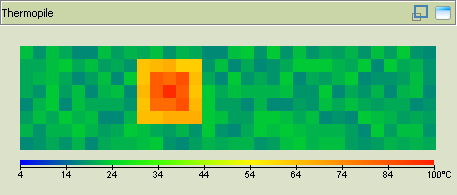
\includegraphics[width=.75\textwidth]{images/thermo}
	\caption{Das Thermopile-Array-Plugin}
	\label{img:plugins:thermo}
\end{figure}

\section{Distanz}
\index{Abstandssensor}
\index{Roboterprofil}
Dieses Plugin zeigt die Werte von Abstandssensoren an. Dieses Plugin bezieht die
Informationen �ber Anzahl und Wertebereich der \seegls{Sensor}en aus dem Roboterprofil. 
In Abbildung \ref{img:plugins:distanz} auf Seite \pageref{img:plugins:distanz}
ist das Plugin in Aktion zu sehen.

\begin{figure}[ht]
	\centering
	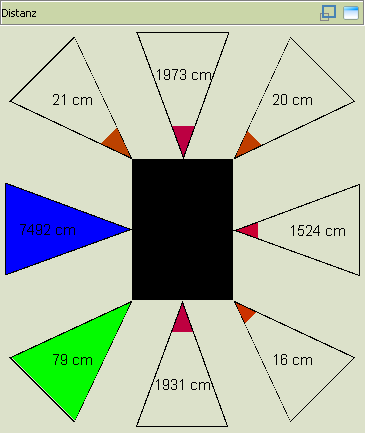
\includegraphics[width=.4\textwidth]{images/distanz}
	\caption{Das Distanz-Plugin}
	\label{img:plugins:distanz}
\end{figure}

\index{Abstandssensor!Infrarot}
\index{Abstandssensor!Ultraschall}
\index{Roboterprofil}
Infratorsensoren werden farblich anders dargestellt als Ultraschallsensoren.
Infratorsensoren werden gr�n und Ultraschallsensoren blau dargestellt, wenn der
Entfernungswert gr��er oder gleich dem Maximum des \seegls{Sensor}s entspricht. Die Farbe
der Sensoranzeigen variiert mit den sich ver�ndernden Werten. Die Einheit in der
die Werte angezeigt werden, werden ebenfalls aus dem Roboterprofil ausgelesen.

\section{Temperatur}
\index{Temperatur}
\index{Thermometer}
\index{Roboterprofil}
Das Temperatur-Plugin zeigt die Werte eines W�rmesensors in Form eines
Thermometers an. Die Markierungen f�r den gelben und roten Bereich erh�lt das
Plugin aus dem Roboterprofil. Die Einheit in der der Wert angezeigt wird, wird
ebenfalls aus dem Roboterprofil ausgelesen. In Abbildung
\ref{img:plugins:temperatur} auf Seite
\pageref{img:plugins:temperatur} ist das Plugin in Aktion zu sehen.

\begin{figure}[htp]
	\centering
	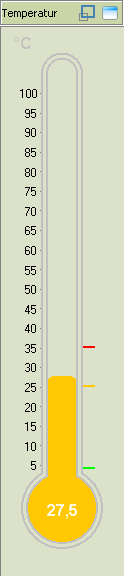
\includegraphics[width=.2\textwidth]{images/temperatur}
	\caption{Das Temperatur-Plugin}
	\label{img:plugins:temperatur}
\end{figure}

\section{CO$_2$}
\index{Kohlendioxid}
\index{CO$_2$}
Dieses \seegls{Sensor}-Plugin zeigt den Verlauf der Werte eines CO$_2$-Sensors an, um so
einen Anstieg des Gases in der umgebenen Luft erkennen zu k�nnen. In Abbildung
\ref{img:plugins:co2} auf Seite \pageref{img:plugins:co2} ist das Plugin in
Aktion zu sehen.

\begin{figure}[ht]
	\centering
	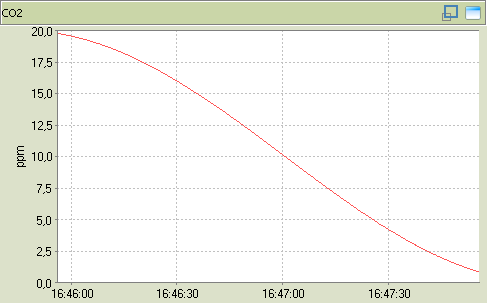
\includegraphics[width=.6\textwidth]{images/co2}
	\caption{Das CO$_2$-Plugin}
	\label{img:plugins:co2}
\end{figure}

\section{Kompass}
\index{Kompass}
\index{Himmelsrichtung}
Das Kompass-Plugin zeigt die aktuell gemessene Himmelsrichtung eines
Kompasssensors in Form eines Kompasses an. Die rote Nadelspitze zeigt die
gemessene Richtung an. In Abbildung \ref{img:plugins:kompass} auf Seite
\pageref{img:plugins:kompass} ist das Plugin in Aktion zu sehen.

\begin{figure}[ht]
	\centering
	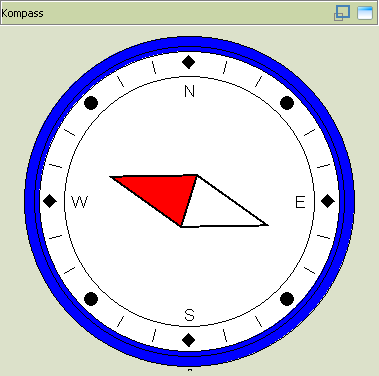
\includegraphics[width=.4\textwidth]{images/kompass}
	\caption{Das Kompass-Plugin}
	\label{img:plugins:kompass}
\end{figure}

\section{Geschwindigkeit}
\index{Geschwindigkeit}
\index{Tachometer}
Dieses Plugin zeigt die gemessene Geschwindigkeit eines Roboters in Form eines
Tachometers an. Die Einheit in der der Wert angezeigt wird, wird
aus dem Roboterprofil ausgelesen. In Abbildung \ref{img:plugins:speed} auf Seite
\pageref{img:plugins:speed} ist das Plugin in Aktion zu sehen.

\begin{figure}[htp]
	\centering
	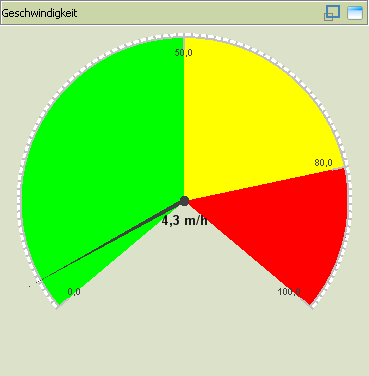
\includegraphics[width=.4\textwidth]{images/speed}
	\caption{Das Geschwindigkeits-Plugin}
	\label{img:plugins:speed}
\end{figure}

\section{Neigung}
\index{Neigung}
\index{Gyroskop}
Dieses Plugin zeigt die gemessenen Werte eines Gyroskops an. Es werden zwei
Werte, die horizontale und die vertikale Neigung, angezeigt. Die Form der
Anzeige ist dem k�nstlichen Horizont, bekannt aus der modernen Avionik,
nachempfunden. Der \enquote{Himmel} ist blau und die \enquote{Erde} gr�n
gef�rbt. In Abbildung \ref{img:plugins:neigung} auf Seite
\pageref{img:plugins:neigung} ist das Plugin in Aktion zu sehen.

\begin{figure}[htp]
	\centering
	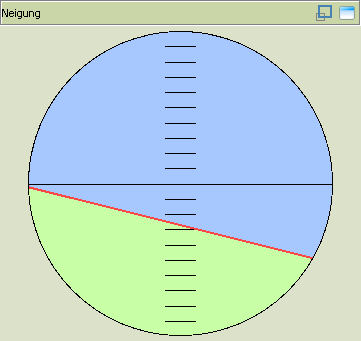
\includegraphics[width=.4\textwidth]{images/neigung}
	\caption{Das Neigungs-Plugin}
	\label{img:plugins:neigung}
\end{figure}

\section{Laserentfernungsmesser}
\index{Laserentfernungsmesser}
Dieses Plugin zeigt Scans eines Laserscaners an. Aus einem solchen Scan
resultiert eine grober Umriss der Umgebung. Die F�llfarbe kann gew�hlt werden.
Eine weitere Option ist, einen Rand um den Umriss zeichnen zu lassen. In
Abbildung \ref{img:plugins:laser} auf Seite \pageref{img:plugins:laser} ist das
Plugin in Aktion zu sehen.

\begin{figure}[htp]
	\centering
	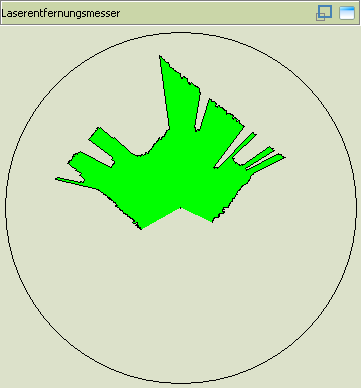
\includegraphics[width=.4\textwidth]{images/laser}
	\caption{Das Laserentfernungsmesser-Plugin}
	\label{img:plugins:laser}
\end{figure}

\section{Nachrichten}
\index{Testerbot}
\index{Sprachausgabe}
\index{Kommandos}
Das Nachrichten-Plugin zeigt die vom \seegls{Testerbot} erzeugten S�tze an. Ist die
Sprachausgabe aktiviert, werden diese S�tze (alle in englischer Sprache) �ber
das Sprachausgabesystem ausgegeben. Des Weiteren exportiert dieses Plugin eine
Funktion, welche mittels der Kommandos aufgerufen werden kann. Wird dieser
Funktion eine Taste zugewiesen, kann durch Dr�cken dieser Taste der Inhalt des
Textfensters gel�scht werden.

\section{Testerbot Protokoll}
\index{Testerbot}
\index{Datenpool}
Das \seegls{Testerbot} Protokoll verarbeitet die vom \seegls{Server} gesendeten Pakete und spielt
die Daten unter den korrekten Schl�sseln in den Datenpool\footnote{F�r weitere
Informationen �ber den Datenpool, lesen sie den
\href{\devguideurl}{Developer Guide}.} ein.

\section{IP Kommunikation}
\index{TCP/IP}
\index{Testerbot}
Dieses Kommunikationsmediumsplugin kann verwendet werden, wenn mit dem Roboter
via \seegls{TCP/IP} kommuniziert werden soll. Der \seegls{Testerbot} kann ausschlie�lich mit
diesem Medium angesprochen werden.
\par
\index{IP-Adresse}
In den Einstellungen ist es m�glich die \seegls{IP-Adresse} und den Port des
Roboters/\seegls{Server}s einzugeben. Die \seegls{IP-Adresse}n werden in IPv4 angegeben.

\section{Serielle Kommunikation}
\index{RS232}
Dieses Plugin realisiert eine Kommunikation �ber eine serielle Schnittstelle
(RS232). In den Einstellungen kann die zu benutzende Schnittstelle definiert und
konfiguriert werden.

\section{Carmen Kommunikation}
\index{Carmen}
\index{Carmen!IPC}
\index{Carmen!Carmen IPC Central Server}
Mit diesem Plugin l�sst sich eine Verbindung zu einem \seegls{Carmen} \seegls{IPC} Central \seegls{Server}
herstellen und Nachrichten an diesen verschicken. In den Einstellungen lassen
sich \seegls{IP-Adresse} und Port des \seegls{Server}s angeben.

\index{Plugins|)}

\chapter{Profile}
\label{sec:sprofile}
\index{Profil}

\index{Roboter}
\index{Profil}
\index{Kommunikation!Spezifikation}
Die \seegls{Profile} sind ein zentraler Bestandteil vom \xirp. \seegls{Profile}, Roboter und
Kommunikationsspezifikationen werden in einzelnen Dateien in \seegls{XML} spezifiziert.
Die \seegls{XML} Struktur wird mittels \enquote{\seegls{JAXB}} und annotierten Java-Klassen in
eine Java-Bean-Struktur �berf�hrt.

Im folgenden Kapitel werden zun�chst die \seegls{XML}-Spezifikationen und im Anschluss
daran die Rep�sentation der \seegls{Profile}, Roboter und Kommunikationsspezifikationen
in den entsprechenden Java-Klassen erl�utert.

Die \seegls{XML}-Dateien wurden mit \seegls{DTDs} definiert. Um beim Einlesen der Dateien eine
Validierung dieser vorzunehmen, wurden die \seegls{DTDs} mittels des Programms
\enquote{Trang}\footnote{Zu finden unter \href{http://www.thaiopensource.com/}
{www.thaiopensource.com}} in \seegls{XSDs} �bersetzt. \enquote{\seegls{JAXB}} ben�tigt diese
Dateien um Validieren zu k�nnen, ob eine Datei g�ltig oder ung�ltig nach den
gegebenen Definitionen ist. Die Beschreibung der Profildateien wird trotzdessen
anhand der \seegls{DTDs} durchgef�hrt, da diese in ihrer Struktur einfacher und
�bersichtlicher sind.

\newpage

\section{Profil}
In den Profildateien, Dateiendung \texttt{pro}, werden die Roboter zugeordnet
die zu diesem \seegls{Profil} geh�ren, sowie die externen Werkzeuge gespeichert.
Dateien dieser Art m�ssen sich im Ordner \texttt{<xirp>/conf/profiles} befinden,
um beim Starten geladen zu werden.

Im folgenden wird die Struktur einer validen Profildatei anhand der DTD
erl�utert.

\begin{xml}[caption=Die DTD von Profildateien (\texttt{pro}), label=lst:prodtd]
<!-- A profile -->
<!ELEMENT profile (robot+, externaltools?)>
<!ATTLIST profile name CDATA #REQUIRED>
<!ATTLIST profile complete (true|false) #REQUIRED>

<!-- A robot -->
<!ELEMENT robot (#PCDATA)>

<!-- The external tools -->
<!ELEMENT externaltools (tool*)>

<!-- A tool -->
<!ELEMENT tool (executable+)>
<!ATTLIST tool name CDATA #REQUIRED>

<!-- A executable -->
<!ELEMENT executable (args?)>
<!ATTLIST executable name CDATA #REQUIRED>
<!ATTLIST executable path CDATA #REQUIRED>
<!ATTLIST executable wait CDATA #REQUIRED>

<!-- The arguments for the executable -->
<!ELEMENT args (#PCDATA)>
\end{xml}

\subsection{<profile>}

Wie zu sehen ist muss mindestens ein Roboter zu geordnet werden:
\texttt{(robot+,}. Die externen Programme sind komplett optional 
\texttt{externaltools?)}. Das Element \texttt{<profile>} hat zwei ben�tigte
Attribute: 

\begin{itemize}
  \item \texttt{name} - Der Name des \seegls{Profils}
  \item \texttt{complete} - \texttt{true} oder \texttt{false}, zeigt
  an, ob das \seegls{Profil} komplett ist (wird intern benutzt).
\end{itemize}

Die im \texttt{<profile>}-Element vorhanden Elemente werden in den folgenden
Abschnitten beschrieben.

\subsubsection{<robot>}

Das Element \texttt{<robot>} muss, um den Roboter
zuweisen und laden zu k�nnen, den Dateinamen des gew�nschten Roboters ohne
Dateiendung enthalten. 

\subsubsection{<externaltools>}

In diesem Bereich werden die externen Programme die dem \seegls{Profil} zugeordnet sind
definiert. Das \texttt{<externaltools>}-Element kann mehrere
\texttt{<tool>}-Elemente enthalten. Jedes \texttt{<tool>}-Element hat ein
Attribut \texttt{name} (der Name des Tools) und eine Folge von mindestens
einem \texttt{<executable>}. Jeder \texttt{<executable>} hat drei
Attribute:

\begin{itemize}
  \item \texttt{name} - Name des ausf�hrbaren Programms (nicht der Dateiname).
  \item \texttt{path} - Kompletter Pfad zum ausf�hrbaren Programm.
  \item \texttt{wait} - Ein Zahlenwert. Die Wartezeit in Millisekunden bis zum Start des
  nachfolgenden Programms.
\end{itemize} 

Zus�tzlich dazu enth�lt jedes \texttt{<executable>} ein oder kein
\texttt{<args>}-Element. In diesem Element werden die Start-Argumente des Programms
als ein String eingetragen. Dieser kann auch leer sein, wenn keine Argumente
vorhanden sind.

\subsection{Valide Profildatei}
Ist die Profildatei als komplett markiert unf valid, wird das \seegls{Profil} in der
Anwendung geladen. Eine valide Profildatei ist in Auflistung
\autoref{lst:profildatei} auf \autopageref{lst:profildatei} zu sehen.

\begin{xml}[caption=Eine valide\, komplette Profildatei, label=lst:profildatei]
<?xml version="1.0" encoding="UTF-8" standalone="yes"?>
<profile complete="true" name="Testing">
    <externaltools>
        <tool name="TestTool">
            <executable wait="1000" path="C:\WINDOWS\NOTEPAD.EXE" name="Notepad">
                <args></args>
            </executable>
            <executable wait="1000" path="C:\WINDOWS\system32\calc.exe" name="Calculator">
                <args></args>
            </executable>
        </tool>
    </externaltools>
    <robot>testerbot</robot>             
</profile>
\end{xml}

\section{Roboter}
In den Roboterdateien, Dateiendung \texttt{bot}, wird ein Roboter komplett
spezifiziert. Von Ma�en, \seegls{Sensor}en und \seegls{Aktuator}en �ber Kommunikationsangaben und
Multimediager�te hin zu den \seegls{Plugins} die f�r den Roboter geladen werden sollen.
Dateien dieser Art m�ssen sich im Ordner \texttt{<xirp>/conf/profiles/robots}
befinden, um beim Starten geladen zu werden. 

Im folgenden wird die Struktur einer validen Profildatei anhand der \seegls{DTD}
erl�utert.

\begin{xml}[caption=Die DTD von Roboterdateien (\texttt{bot}), label=img:botdtd]
<!-- Structure of <robot> -->
<!ELEMENT robot (robotspecs,actuators,powersource+,sensorgroup*,communicationspecification,multimedia?,plugins?)>
<!ATTLIST robot name CDATA #REQUIRED>
<!ATTLIST robot type (WHEEL|WALK|FLY|OTHER) #REQUIRED>
<!ATTLIST robot completed (true|false) #REQUIRED>

<!-- Measurements of the torso -->
<!ELEMENT robotspecs (height,width,length,weight)>

<!-- The height of the robot -->
<!ELEMENT height (#PCDATA)> 
<!ATTLIST height unit (MILLIMETER|CENTIMETER|DECIMETER|METER) #REQUIRED>

<!-- The width of the robot -->
<!ELEMENT width (#PCDATA)>
<!ATTLIST width unit (MILLIMETER|CENTIMETER|DECIMETER|METER) #REQUIRED>

<!-- The length of the robot -->
<!ELEMENT length (#PCDATA)>
<!ATTLIST length unit (MILLIMETER|CENTIMETER|DECIMETER|METER) #REQUIRED>

<!-- The weight of the robot -->
<!ELEMENT weight (#PCDATA)>
<!ATTLIST weight unit (GRAM|KILOGRAM|TON) #REQUIRED>

<!-- Actuators -->
<!ELEMENT actuators (actuatorgroup+)>
<!ATTLIST actuators count CDATA #REQUIRED>

<!-- A group of actuators -->
<!ELEMENT actuatorgroup (actuator+)>
<!ATTLIST actuatorgroup name CDATA #REQUIRED>

<!-- A actuator -->
<!ELEMENT actuator (minimum,maximum)>
<!ATTLIST actuator id CDATA #REQUIRED>
<!ATTLIST actuator name CDATA #REQUIRED>
<!ATTLIST actuator unit (DEGREE|PERCENT|RPM) #REQUIRED>

<!-- Power sources -->
<!ELEMENT powersource (#PCDATA)>
<!ATTLIST powersource warningValue CDATA #REQUIRED>
<!ATTLIST powersource max CDATA #REQUIRED>
<!ATTLIST powersource unit (AMPERE|VOLT|FARAD|PERCENT|CCM) #REQUIRED>
<!ATTLIST powersource datapoolKey CDATA #REQUIRED>

<!-- Sensor groups -->
<!ELEMENT sensorgroup (sensor+)>
<!ATTLIST sensorgroup visible (true|false) #REQUIRED>
<!ATTLIST sensorgroup longName CDATA #REQUIRED>
<!ATTLIST sensorgroup datapoolKey CDATA #REQUIRED>

<!-- Sensors -->
<!ELEMENT sensor (sensorspecs)>
<!ATTLIST sensor id CDATA #REQUIRED>
<!ATTLIST sensor subKey CDATA #REQUIRED>
<!ATTLIST sensor unit (DEGREE|PERCENT|RPM|PARTICLES_PER_MILLION|CENTIMETER|KELVIN|CELSIUS|FAHRENHEIT|MILES_PER_HOUR|KILOMETERS_PER_HOUR|METERS_PER_HOUR|METERS_PER_MINUTE|CENTIMETERS_PER_HOUR|CENTIMETERS_PER_MINUTE) #REQUIRED>

<!-- Specs of a sensor -->
<!ELEMENT sensorspecs (position,minimum,maximum,option*)>

<!-- The position of the sensor -->
<!ELEMENT position EMPTY>
<!ATTLIST position attached (TORSO|EXTREMITY) #REQUIRED>
<!ATTLIST position side (FRONT|REAR|LEFT|RIGHT|INSIDE|TOP|BOTTOM) #REQUIRED>
<!ATTLIST position x CDATA #REQUIRED>
<!ATTLIST position y CDATA #REQUIRED>

<!-- A minimum -->
<!ELEMENT minimum (#PCDATA)>

<!-- A maximum -->
<!ELEMENT maximum (#PCDATA)>

<!-- A option -->
<!ELEMENT option (#PCDATA)>
<!ATTLIST option name CDATA #REQUIRED>

<!-- A fully qualified class name -->
<!ELEMENT class (#PCDATA)>

<!-- Name of the comm-specs file -->
<!ELEMENT communicationspecification (#PCDATA)>

<!-- Multimedia -->
<!ELEMENT multimedia (video?,audio?)>

<!-- Video devices -->
<!ELEMENT video (camera*,display*)>
<!ATTLIST video simultaneous (true|false) #REQUIRED>

<!-- A camera -->
<!ELEMENT camera (#PCDATA)>

<!-- A display -->
<!ELEMENT display (#PCDATA)>

<!-- Audio devices -->
<!ELEMENT audio (microphone*,speaker*)>

<!-- A microphone -->
<!ELEMENT microphone (#PCDATA)>

<!-- A speaker -->
<!ELEMENT speaker (#PCDATA)>

<!-- The plugins -->
<!ELEMENT plugins (plugin+)>

<!-- A plugin -->
<!ELEMENT plugin (class,sensorname*,usemultimedia?,option*)>
<!ATTLIST plugin name CDATA #REQUIRED>

<!-- Name of a sensor which is displayed by a plugin -->
<!ELEMENT sensorname (#PCDATA)>

<!-- Flag, indicating if the plugin uses multiumedia devices -->
<!ELEMENT usemultimedia (true|false)>
\end{xml}

\subsection{<robot>}
In \autoref{lst:botdtd:robot} auf \autopageref{lst:botdtd:robot} ist die
Definition des Elements \texttt{<robot>} zu sehen.

\begin{xml}[caption=DTD: Definition von \texttt{<robot>}, label=lst:botdtd:robot]
<!ELEMENT robot (robotspecs,actuators,powersource+,sensorgroup*,communicationspecification,multimedia?,plugins?)>
<!ATTLIST robot name CDATA #REQUIRED>
<!ATTLIST robot type (WHEEL|WALK|FLY|OTHER) #REQUIRED>
<!ATTLIST robot completed (true|false) #REQUIRED>
\end{xml}

Das \texttt{<robot>}-Element enth�lt drei Attribute:

\begin{itemize}
  \item \texttt{name} - Name des Roboters.
  \item \texttt{type} - Der Typ des Roboters. Hier kann zwischen vier M�glichkeiten
  gew�hlt werden:
  \begin{itemize}
    \item \texttt{WHEEL} - Der Roboter hat R�der.
    \item \texttt{WALK} - Der Roboter hat Beine.
    \item \texttt{FLY} - Der Roboter fliegt.
    \item \texttt{OTHER} - Der Roboter pass in keine der drei vorherigen
    Kategorien.
  \end{itemize}
  \item \texttt{completed} - \texttt{true} oder \texttt{false}, zeigt
  an, ob der Roboter komplett ist (wird intern benutzt).  
\end{itemize}

Innerhalb des \texttt{<robot>}-Elements k�nnen die folgenden Elemente in
unterschiedlicher Anzahl vorkommen:

\begin{itemize}
  \item \texttt{<robotspecs>} - Die Roboterspezifikation, muss genau einmal
  vorkommen.
  \item \texttt{<actuators>} - Die \seegls{Aktuator}en des Roboters, muss genau einmal
  vorkommen.
  \item \texttt{<powersource>} -  Die Energiequellen des Roboters, muss
  mindestens einmal vorkommen.
  \item \texttt{<sensorgroup>} - Die gruppierten Sensoren, muss garnicht und
  kann mehrfach vorkommen.
  \item \texttt{<communicationspecification>} - Die Kommunikation des roboters,
  muss genau einmal vorkommen.
  \item \texttt{<multimedia>} - Die Multimediager�te des Roboters, kann garnicht
  oder genau einmal vorkommen.
  \item \texttt{<plugins>} - Die Plugins des Roboters, kann garnicht oder genau
  einmal vorkommen.
\end{itemize}

Die Definitionen dieser Elemente wird in den folgenden Abschnitten erl�utert.

\subsubsection{<robotspecs>}
\label{sec:robotspecs}
In \autoref{lst:botdtd:robotspecs} auf \autopageref{lst:botdtd:robotspecs} ist die
Definition des Elements \texttt{<robotspecs>} zu sehen.

\begin{xml}[caption=DTD: Definition von \texttt{<robotspecs>},
label=lst:botdtd:robotspecs] 
<!ELEMENT robotspecs (height,width,length,weight)>

<!ELEMENT height (#PCDATA)> 
<!ATTLIST height unit (MILLIMETER|CENTIMETER|DECIMETER|METER) #REQUIRED>

<!ELEMENT width (#PCDATA)>
<!ATTLIST width unit (MILLIMETER|CENTIMETER|DECIMETER|METER) #REQUIRED>

<!ELEMENT length (#PCDATA)>
<!ATTLIST length unit (MILLIMETER|CENTIMETER|DECIMETER|METER) #REQUIRED>

<!ELEMENT weight (#PCDATA)>
<!ATTLIST weight unit (GRAM|KILOGRAM|TON) #REQUIRED>
\end{xml}

Innerhalb des \texttt{<robotspecs>}-Elementes befinden sich vier weitere
Elemente:

\begin{itemize}
  \item \texttt{<height>} - Die H�he des Torsos, muss genau einmal vorkommen.
  \item \texttt{<width>} - Die Breite des Torsos, muss genau einmal vorkommen.
  \item \texttt{<length>} - Die L�nge des Torsos, muss genau einmal vorkommen.
  \item \texttt{<weight>} - Das Gewicht des Roboters, muss genau einmal vorkommen.
\end{itemize}

Jedes dieser Elemente hat das ben�tigte Attribut \texttt{unit}. Hier kann bei
den L�ngenangaben \texttt{<height>}, \texttt{<width>} und \texttt{<length>} 
zwischen folgende Werten gew�hlt werden:

\begin{itemize}
  \item \texttt{MILLIMETER} - Ma�einheit ist dann Millimeter.
  \item \texttt{CENTIMETER} - Ma�einheit ist dann Zentimeter.
  \item \texttt{DECIMETER} - Ma�einheit ist dann Dezimeter.
  \item \texttt{METER} - Ma�einheit ist dann Meter.
\end{itemize}

Bei der Gewichtsangabe -- \texttt{<weight>} -- kann zwischen folgenden Werten
gew�hlt werden:

\begin{itemize}
  \item \texttt{GRAM} - Ma�einheit ist dann Gramm.
  \item \texttt{KILOGRAM} - Ma�einheit ist dann Kilogramm.
  \item \texttt{TON} - Ma�einheit ist dann Tonnen.
\end{itemize}

In \autoref{lst:botdtd:robotspecs:valid} auf
\autopageref{lst:botdtd:robotspecs:valid} ist ein valider
\texttt{<robotspecs>}-Bereich zu sehen.

\begin{xml}[caption=Ein valides \texttt{<robotspecs>-Element},
label=lst:botdtd:robotspecs:valid] 
<robotspecs>
    <height unit="MILLIMETER">200.0</height>
    <width unit="MILLIMETER">500.0</width>
    <length unit="MILLIMETER">700.0</length>
    <weight unit="KILOGRAM">5.0</weight>
</robotspecs>
\end{xml}

\subsubsection{<actuators>}
In \autoref{lst:botdtd:actuators} auf \autopageref{lst:botdtd:actuators} ist die
die Definition des Elements \texttt{<actuators>} zu sehen.

\begin{xml}[caption=DTD: Definition von \texttt{<actuators>}, 
label=lst:botdtd:actuators] 
<!ELEMENT actuators (actuatorgroup+)>
<!ATTLIST actuators count CDATA #REQUIRED>

<!ELEMENT actuatorgroup (actuator+)>
<!ATTLIST actuatorgroup name CDATA #REQUIRED>

<!ELEMENT actuator (minimum,maximum)>
<!ATTLIST actuator id CDATA #REQUIRED>
<!ATTLIST actuator name CDATA #REQUIRED>
<!ATTLIST actuator unit (DEGREE|PERCENT|RPM) #REQUIRED>

<!ELEMENT minimum (#PCDATA)>

<!ELEMENT maximum (#PCDATA)>
\end{xml}

Das \texttt{<actuators>}-Element besitzt das Attribut \texttt{count}. In diesem
befindet sich die Anzahl der vorhandenen \seegls{Aktuator}en. Dieser Wert wird intern
gesetzt. Des Weiteren kann das Element mindestens einen
\texttt{<actuatorgroup>}-Tag enthalten.

Das \texttt{<actuatorgroup>}-Element gruppiert \seegls{Aktuator}en, z.B. k�nnen sie alle
Servos eines Beines als Gruppe \enquote{leg} zusammengefasst werden. Das
Element besitzt das Attribut \texttt{name}, welches den Namen der Gruppe
wiedergibt. Eine Gruppe muss mindestens ein \texttt{<actuator>}-Element
beinhalten. 

Das \texttt{<actuator>}-Element hat drei Attribute:

\begin{itemize}
  \item \texttt{id} - Erkennungsmarke des \seegls{Aktuator}s (ein Zahlenwert).
  \item \texttt{name} - Der Name des \seegls{Aktuator}s.
  \item \texttt{unit} - Die Ma�einheit in der die Werte des \seegls{Aktuator}s gemessen
  werden. Es stehen folgende ma�einheiten zur Auswahl:
  \begin{itemize}
    \item \texttt{DEGREE} - Einheit wird in Grad angegeben.
    \item \texttt{PERCENT} - Einheit wird in Prozent angegeben.
    \item \texttt{RPM} - Einheit wird in Umdrehungen pro Minute.
  \end{itemize}
\end{itemize}

Zus�tzlich hat jedes \texttt{<actuator>}-Element zwei weitere Elemente, die beide
ein einziges Mal vorhanden sein m�ssen:

\begin{itemize}
  \item \texttt{<minimum>} - Der minimale Wert den der \seegls{Aktuator} erreichen kann,
  die Einheit entspricht der Angabe in \texttt{unit} des
  \texttt{<actuator>}-Elements.
  \item \texttt{<maximum>} - Der maximale Wert den der \seegls{Aktuator} erreichen kann,
  die Einheit entspricht der Angabe in \texttt{unit} des
  \texttt{<actuator>}-Elements.
\end{itemize}

In \autoref{lst:botdtd:actuators:valid} auf
\autopageref{lst:botdtd:actuators:valid} ist ein valider
\texttt{<actuators>}-Bereich zu sehen.

\begin{xml}[caption=Ein valides \texttt{<actuators>-Element},
label=lst:botdtd:actuators:valid] 
<actuators count="2">
    <actuatorgroup name="drive">
        <actuator name="left" unit="PERCENT" id="0">
            <minimum>0.0</minimum>
            <maximum>100.0</maximum>
        </actuator>
        <actuator name="right" unit="PERCENT" id="1">
            <minimum>0.0</minimum>
            <maximum>100.0</maximum>
        </actuator>
    </actuatorgroup>
</actuators>
\end{xml}

\subsubsection{<powersource>}
In \autoref{lst:botdtd:powersource} auf \autopageref{lst:botdtd:powersource}
ist die Definition des Elements \texttt{<actuators>} zu sehen.

\begin{xml}[caption=DTD: Definition von \texttt{<powersource>}, 
label=lst:botdtd:powersource] 
<!ELEMENT powersource (#PCDATA)>
<!ATTLIST powersource warningValue CDATA #REQUIRED>
<!ATTLIST powersource max CDATA #REQUIRED>
<!ATTLIST powersource unit (AMPERE|VOLT|FARAD|PERCENT|CCM) #REQUIRED>
<!ATTLIST powersource datapoolKey CDATA #REQUIRED>
\end{xml}

Von dem \texttt{<powersource>}-Elemente muss mindestens eins vorhanden sein. Es
hat vier Attribute:

\begin{itemize}
  \item \texttt{warningValue} - Ein Zahlenwert; zeigt den Wert an ab dem eine
  Warnung ausgegenen soll, dass die Energiequelle bald keine Energie mehr
  liefert.
  \item \texttt{max} - Der maximale Wert der Energiequelle.
  \item \texttt{unit} - Die Einheit in der \texttt{warningValue} und
  \texttt{max} gemessen werden. Es stehen f�nf Werte zur Auswahl:
  \begin{itemize}
    \item \texttt{AMPERE} - Die Ma�einheit ist Ampere.
    \item \texttt{VOLT} - Die Ma�einheit ist Volt.
    \item \texttt{FARAD} - Die Ma�einheit ist Farad.
    \item \texttt{PERCENT} - Die Ma�einheit ist Prozent.
    \item \texttt{CCM} - Die Ma�einheit ist Kubikzentimeter.
  \end{itemize}
  \item \texttt{datapoolKey} - Der Schl�sel unter dem die Werte der
  Energiequelle in den Datenpool\index{Datenpool} eingespielt werden.
\end{itemize}

Der Name der Energiequelle wird im \enquote{value}-Bereich des Elements angegeben:
\newline\texttt{<powersource>Name</powersource>}.

In \autoref{lst:botdtd:powersource:valid} auf
\autopageref{lst:botdtd:powersource:valid} ist ein valider
\texttt{<powersource>}-Bereich mit zwei Energiequellen zu sehen.

\begin{xml}[caption=Ein valides \texttt{<powersource>-Element},
label=lst:botdtd:powersource:valid] 
<powersource datapoolKey="battery1" unit="AMPERE" max="5.0" warningValue="0.5">Battery1</powersource>
<powersource datapoolKey="battery2" unit="AMPERE" max="5.0" warningValue="0.5">Battery2</powersource>
\end{xml}

\subsubsection{<sensorgroup>}
\label{sec:sensorgroup}
In \autoref{lst:botdtd:sensorgroup} auf \autopageref{lst:botdtd:sensorgroup} ist die
Definition des Elements \texttt{<sensorgroup>} zu sehen.

\begin{xml}[caption=DTD: Definition von \texttt{<sensorgroup>}, 
label=lst:botdtd:sensorgroup] 
<!ELEMENT sensorgroup (sensor+)>
<!ATTLIST sensorgroup visible (true|false) #REQUIRED>
<!ATTLIST sensorgroup longName CDATA #REQUIRED>
<!ATTLIST sensorgroup datapoolKey CDATA #REQUIRED>

<!ELEMENT sensor (sensorspecs)>
<!ATTLIST sensor id CDATA #REQUIRED>
<!ATTLIST sensor subKey CDATA #REQUIRED>
<!ATTLIST sensor unit (DEGREE|PERCENT|RPM|PARTICLES_PER_MILLION|CENTIMETER|KELVIN|CELSIUS|FAHRENHEIT|MILES_PER_HOUR|KILOMETERS_PER_HOUR|METERS_PER_HOUR|METERS_PER_MINUTE|CENTIMETERS_PER_HOUR|CENTIMETERS_PER_MINUTE) #REQUIRED>

<!ELEMENT sensorspecs (position,minimum,maximum,option*)>

<!ELEMENT position EMPTY>
<!ATTLIST position attached (TORSO|EXTREMITY) #REQUIRED>
<!ATTLIST position side (FRONT|REAR|LEFT|RIGHT|INSIDE|TOP|BOTTOM) #REQUIRED>
<!ATTLIST position x CDATA #REQUIRED>
<!ATTLIST position y CDATA #REQUIRED>

<!ELEMENT minimum (#PCDATA)>

<!ELEMENT maximum (#PCDATA)>

<!ELEMENT option (#PCDATA)>
<!ATTLIST option name CDATA #REQUIRED>
\end{xml}

Das \texttt{<sensorgroup>}-Element muss garnicht und kann mehrfach vorhanden
sein. Es gruppiert \seegls{Sensoren} eines Typs, z.B. k�nnen alle
Infrarotabstandssensoren so zusammengefasst werden. Jedes Gruppenelement enth�lt
mindetsens ein \texttt{<sensor>}-Element. Des Weiteren hat das Gruppenelement
drei Attribute:

\begin{itemize}
  \item \texttt{visible} - \texttt{true} oder \texttt{false}; zeigt an, ob die
  Gruppe sichtbar sein soll, oder nicht.
  \item \texttt{longName} - Der Name der Gruppe in Langform.
  \item \texttt{datapoolKey} - Dies ist der Prefix f�r den kompletten
  Schl�ssel unter dem der Werte eines \seegls{Sensor}s in den Datenpool\index{Datenpool}
  eingespielt werden soll. Der Schl�ssel setzt sich aus diesem Key und dem
  \texttt{subKey} des \seegls{Sensor}s folgenderma�en zusammen:\\
  \texttt{<datapoolKey>\_<subKey>}.
\end{itemize}

Das \texttt{<sensor>}-Element enth�lt genau ein \texttt{<sensorspecs>}-Element
und hat drei Attribute:

\begin{itemize}
  \item \texttt{id} - Erkennungsmarke des Sensors als Zahlenwert.
  \item \texttt{subKey} - Der zweite Teil des Schl�ssels unter dem der Wert des
  Sensors in den Datenpool\index{Datenpool} eingespielt werden soll. Der
  Schl�ssel setzt sich aus diesem Key und dem \texttt{datapoolKey} der
  Sensorgruppe folgenderma�en zusammen: \\
     \texttt{<datapoolKey>\_<subKey>}.
  \item \texttt{unit} - Die Ma�einheit des Wertes den der Sensor liefert. Hier
  gibt es 14 Auswahlm�glichkeiten:
  \begin{itemize}
    \item \texttt{DEGREE} - Die Ma�einheit ist Grad.
    \item \texttt{PERCENT} - Die Ma�einheit ist Prozent.
    \item \texttt{RPM} - Die Ma�einheit ist Undrehungen pro Minute. 
    \item \texttt{PARTICLES\_PER\_MILLION} - Die Ma�einheit ist Partikel pro
    Million. 
    \item \texttt{CENTIMETER} - Die Ma�einheit ist Zentimeter. 
    \item \texttt{KELVIN} - Die Ma�einheit ist Grad Kelvin (�K).  
    \item \texttt{CELSIUS} - Die Ma�einheit ist Grad Celsius (�C). 
    \item \texttt{FAHRENHEIT} - Die Ma�einheit ist Grad Fahrenheit (�F). 
    \item \texttt{MILES\_PER\_HOUR} - Die Ma�einheit ist Meilen pro Stunde. 
    \item \texttt{KILOMETERS\_PER\_HOUR} - Die Ma�einheit ist Kilometer pro
    Stunde. 
    \item \texttt{METERS\_PER\_HOUR} - Die Ma�einheit ist Meter pro Stunde. 
    \item \texttt{METERS\_PER\_MINUTE} - Die Ma�einheit ist Meter pro Minute. 
    \item \texttt{CENTIMETERS\_PER\_HOUR} - Die Ma�einheit ist Centimeter pro
    Stunde.
    \item \texttt{CENTIMETERS\_PER\_MINUTE} - Die Ma�einheit ist Centimeter pro
    Minute.
  \end{itemize}
\end{itemize}

Das \texttt{<sensorspecs>}-Element enth�lt drei Elemente, jedes muss genau
einmal vorhanden sein:

\begin{itemize}
  \item \texttt{<position>} - Die Position an dem der Sensor befestigt ist.
  \item \texttt{<minimum>} - Der minimale Wert den der Sensor liefern kann,
  die Einheit entspricht der Angabe in \texttt{unit} des
  \texttt{<sensor>}-Elements.
  \item \texttt{<maximum>} - Der maximale Wert den der Sensor liefern kann,
  die Einheit entspricht der Angabe in \texttt{unit} des
  \texttt{<sensor>}-Elements.
\end{itemize}

Das \texttt{<sensorspecs>}-Element kann zus�tzlich mehrere
\texttt{<option>}-Elemente enthalten. Eine Option wird folgenderma�en
angegeben: \newline\texttt{<option name="Name der Option''>Wert der Option</option>}.

Das in der Sensorspezifikation enthaltene \texttt{position}-Element ist ein
leeres Element, d.h. es kann mit \texttt{<position/>}) angegeben werden). Es
enth�lt lediglich vier Attribute:

\begin{itemize}
  \item \texttt{attached} - Hiermit wird angegeben, wo der Sensor befestigt
  ist. Es stehen zwei Werte zur Auswahl:
  \begin{itemize}
    \item \texttt{TORSO} - Der Sensor ist am Torso befestigt.
    \item \texttt{EXTREMITY} - Der Sensor befindet sich an einer Extremit�t,
    z.B. ein Drucksensor am Fu� eines Laufroboters.
  \end{itemize}
  \item \texttt{side} - Hiermit wird die Seite angegeben, an der der Sensor
  angebracht ist. Es stehen sieben Werte zur Auswahl:
  \begin{itemize}
    \item \texttt{FRONT} - Der Sensor ist an der Vorderseite angebracht.
    \item \texttt{REAR} - Der Sensor ist an der R�ckseite angebracht.
    \item \texttt{LEFT} - Der Sensor ist auf der linken Seite angebracht.
    \item \texttt{RIGHT} - Der Sensor ist auf der rechten Seite angebracht.
    \item \texttt{INSIDE} - Der Sensor ist im Inneren angebracht.
    \item \texttt{TOP} - Der Sensor ist auf der Oberseite angebracht.
    \item \texttt{BOTTOM} - Der Sensor ist auf an der Unterseite angebracht.
  \end{itemize}
  \item \texttt{x} - Numerischer Wert; gibt die Verschiebung in X-Richtung des
  Sensors vom Ursprung aus an. Dieser ist immer \enquote{unten links}. 
  Abbildung \autoref{img:profile:ursprung} auf 
  \autopageref{img:profile:ursprung} verdeutlicht wo genau der Ursprung ist
  und was ein positiver Wert f�r die Verschiebung bedeutet. Negative Werte sind
  nicht erlaubt.
  \item \texttt{y} - Numerischer Wert; gibt die Verschiebung in Y-Richtung des
  Sensors vom Ursprung aus an. Dieser ist immer \enquote{unten links}. 
  Abbildung \autoref{img:profile:ursprung} auf 
  \autopageref{img:profile:ursprung} verdeutlicht wo genau der Ursprung ist
  und was ein positiver Wert f�r die Verschiebung bedeutet. Negative Werte sind
  nicht erlaubt.
\end{itemize}

\kfig{ursprung}{.45}{Der Ursprung f�r die Verschiebung eines Sensors}
{img:profile:ursprung}

In \autoref{lst:botdtd:sensorgroup:valid} auf
\autopageref{lst:botdtd:sensorgroup:valid} ist ein valider
\texttt{<sensorgroup>}-Bereich zu sehen.

\begin{xml}[caption=Ein valides \texttt{<sensorgroup>-Element},
label=lst:botdtd:sensorgroup:valid] 
<sensorgroup datapoolKey="gyro" longName="Gyroscope" visible="true">
    <sensor subKey="roll_unique" unit="PERCENT" id="0">
        <sensorspecs>
            <position y="350" x="250" side="INSIDE" attached="TORSO"/>
            <minimum>0.0</minimum>
            <maximum>0.0</maximum>
            <option name="direction">roll</option>
        </sensorspecs>
    </sensor>
    <sensor subKey="nick_unique" unit="PERCENT" id="1">
        <sensorspecs>
            <position y="350" x="250" side="INSIDE" attached="TORSO"/>
            <minimum>0.0</minimum>
            <maximum>0.0</maximum>
            <option name="direction">nick</option>
        </sensorspecs>
    </sensor>
</sensorgroup>
\end{xml}

\subsubsection{<communicationspecification>}
\label{sec:comspecs}
In \autoref{lst:botdtd:communicationspecification} auf
\autopageref{lst:botdtd:communicationspecification} ist die
Definition des Elements \texttt{<communicationspecification>} zu sehen.

\begin{xml}[caption=DTD: Definition von \texttt{<communicationspecification>},
label=lst:botdtd:communicationspecification]
<!ELEMENT communicationspecification (#PCDATA)>
\end{xml}

In \texttt{value}-Teil des \texttt{<communicationspecification>}-Elements wird
der Dateiname der \index{Kommunikation!Spezifikation}Kommunikationsspezifikationsdatei ohne Dateiendung angegeben.

In \autoref{lst:botdtd:communicationspecification:valid} auf
\autopageref{lst:botdtd:communicationspecification:valid} ist ein valider
\texttt{<communicationspecification>}-Bereich zu sehen.

\begin{xml}[caption=Ein valides \texttt{<communicationspecification>-Element},
label=lst:botdtd:communicationspecification:valid] 
<communicationspecification>testerbot_spec</communicationspecification>
\end{xml}

\subsubsection{<multimedia>}
In \autoref{lst:botdtd:multimedia} auf \autopageref{lst:botdtd:multimedia} ist
die Definition des Elemets \texttt{<multimedia>} zu sehen.

\begin{xml}[caption=DTD: Definition von \texttt{<multimedia>}, 
label=lst:botdtd:multimedia] 
<!ELEMENT multimedia (video?,audio?)>

<!ELEMENT video (camera*,display*)>
<!ATTLIST video simultaneous (true|false) #REQUIRED>

<!ELEMENT camera (#PCDATA)>

<!ELEMENT display (#PCDATA)>

<!ELEMENT audio (microphone*,speaker*)>

<!ELEMENT microphone (#PCDATA)>

<!ELEMENT speaker (#PCDATA)>
\end{xml}

Das \texttt{<multimedia>}-Element muss nicht und kann einmal verwendet werden.
Es kann zwei weitere Elemente enthalten die wiederum jeweils zwei weitere
Elemente enthalten k�nnen.

\begin{itemize}
  \item \texttt{<video>} - Dieses Element enth�lt die Videoger�te des Roboters
  und kann garnicht oder einmal vorkommen.
  \begin{itemize}
    \item \texttt{camera} - Hier wird im \texttt{value}-Teil des Elementes der
    Name der Kamera angegeben.
    \item \texttt{display} - Hier wird im \texttt{value}-Teil des Elements der
    Name des Displays angegeben.
  \end{itemize}
  \item \texttt{<audio>} - Dieses Element enth�lt die Audioger�te des Roboters
  und kann garnicht oder einmal vorkommen.
  \begin{itemize}
    \item \texttt{microphone} - Hier wird im \texttt{value}-Teil des Elements
    der Name des Mikrofons angegeben.
    \item \texttt{speaker} - Hier wird im \texttt{value}-Teil des Elements der
    Name des Lautspredcher angegeben.
  \end{itemize} 
\end{itemize}

Das \texttt{<video>}-Element besitzt zus�tzlich noch das Attribut
\texttt{simultaneous}. Hier kann \texttt{true} oder \texttt{false} angegeben
werden. Es zeigt an, ob die Kamerabilder (falls mehr als eine vorhanden)
gleichzeitig angezeigt werden k�nnen.

In \autoref{lst:botdtd:multimedia:valid} auf
\autopageref{lst:botdtd:multimedia:valid} ist ein valider
\texttt{<multimedia>}-Bereich zu sehen.

\begin{xml}[caption=Ein valides \texttt{<multimedia>-Element},
label=lst:botdtd:multimedia:valid] 
<multimedia>
    <video simultaneous="false">
        <camera>Front Cam</camera>
        <display>Front Display</display>
    </video>
    <audio>
    	<microphone>Front Mic</microphone>
    	<speaker>Front Speaker</speaker>
    </audio>
</multimedia>
\end{xml}

\subsubsection{<plugins>}
\label{sec:profile:plugins}
In \autoref{lst:botdtd:plugins} auf \autopageref{lst:botdtd:plugins} ist die
Definition des Elements \texttt{<plugins>} zu sehen.

\begin{xml}[caption=DTD: Definition von \texttt{<plugins>}, 
label=lst:botdtd:plugins] 
<!ELEMENT plugins (plugin+)>

<!ELEMENT plugin (class,sensorname*,usemultimedia?,option*)>
<!ATTLIST plugin name CDATA #REQUIRED>

<!ELEMENT option (#PCDATA)>
<!ATTLIST option name CDATA #REQUIRED>

<!ELEMENT class (#PCDATA)>

<!ELEMENT sensorname (#PCDATA)>

<!ELEMENT usemultimedia (true|false)>
\end{xml}

Das \texttt{<plugins>}-Element kann garnicht oder einmal vorkommen. Es enth�lt
mindestens ein oder mehere \texttt{<plugin>}-Elemente. Das \texttt{<plugin>}
kann bis zu vier weitere Elemente enthalten:

\begin{itemize}
  \item \texttt{class} - Das Element muss einmal vorhanden sein. Es enth�lt in
  seinem \texttt{value}-Teil den kompletten Klassennamen des zu ladenden
  \seegls{Plugins}.
  \item \texttt{sensorname} - Das Element kann garnicht oder mehrfach vorhanden
  sein. Es enth�lt ins einem \texttt{value}-Teil den Namen (\texttt{longName})
  einer Sensorgruppe um einem \seegls{Plugin}, welches Sensorenwerte nutzt die Zuordnung
  zu erleichtern.
  \item \texttt{usemultimedia} - Das Element kann garnicht oder einmal vorhanden
  sein. Es enth�lt in seinem \texttt{value}-Teil entweder \texttt{true} oder
  \texttt{false}. Dies zeigt an, ob das \seegls{Plugin} die Multimediager�te des Roboters
  nutzt oder nicht.
  \item \texttt{option} - Das Element kann garnicht oder mehrfach vorhanden
  sein. Es gibt eine zus�tzliche Option an die dem \seegls{Plugin} �bergeben werden kann.
  Eine Option wird folgenderma�en angegeben: \texttt{<option name="Name der
  Option">Wert der Option</option>}.
\end{itemize} 

In \autoref{lst:botdtd:plugins:valid} auf
\autopageref{lst:botdtd:plugins:valid} ist ein valider
\texttt{<plugins>}-Bereich zu sehen.

\begin{xml}[caption=Ein valides \texttt{<plugins>-Element},
label=lst:botdtd:plugins:valid] 
<plugins>
     <plugin name="Gyro">
        <class>de.unibremen.rr.plugins.sensors.pitch.PitchDisplay</class>
        <sensorname>Gyroscope</sensorname>
        <usemultimedia>false</usemultimedia>
        <option name="color">red</option>
    </plugin>
</plugins>        
\end{xml}

\subsection{Valide Roboterdatei}
F�gt man alle besprochenen Teile zu dem \texttt{<roboter>}-Element hinzu erh�lt
man die in \autoref{lst:botdtd:valid} auf \autopageref{lst:botdtd:valid} zu
sehende valide Roboterdatei.

\begin{xml}[caption=Eine valide Roboterdatei, label=lst:botdtd:valid]
<?xml version="1.0" encoding="UTF-8" standalone="yes"?>
<robot type="WHEEL" name="TesterBot" completed="true">
	<robotspecs>
	    <height unit="MILLIMETER">200.0</height>
	    <width unit="MILLIMETER">500.0</width>
	    <length unit="MILLIMETER">700.0</length>
	    <weight unit="KILOGRAM">5.0</weight>
	</robotspecs>
	<actuators count="2">
	    <actuatorgroup name="drive">
	        <actuator name="left" unit="PERCENT" id="0">
	            <minimum>0.0</minimum>
	            <maximum>100.0</maximum>
	        </actuator>
	        <actuator name="right" unit="PERCENT" id="1">
	            <minimum>0.0</minimum>
	            <maximum>100.0</maximum>
	        </actuator>
	    </actuatorgroup>
	</actuators>
	<powersource datapoolKey="battery1" unit="AMPERE" max="5.0" warningValue="0.5">Battery1</powersource>
	<powersource datapoolKey="battery2" unit="AMPERE" max="5.0" warningValue="0.5">Battery2</powersource>
	<sensorgroup datapoolKey="gyro" longName="Gyroscope" visible="true">
	    <sensor subKey="roll_unique" unit="PERCENT" id="0">
	        <sensorspecs>
	            <position y="350" x="250" side="INSIDE" attached="TORSO"/>
	            <minimum>0.0</minimum>
	            <maximum>0.0</maximum>
	            <option name="direction">roll</option>
	        </sensorspecs>
	    </sensor>
	    <sensor subKey="nick_unique" unit="PERCENT" id="1">
	        <sensorspecs>
	            <position y="350" x="250" side="INSIDE" attached="TORSO"/>
	            <minimum>0.0</minimum>
	            <maximum>0.0</maximum>
	            <option name="direction">nick</option>
	        </sensorspecs>
	    </sensor>
	</sensorgroup>
	<communicationspecification>testerbot_spec</communicationspecification>
	<multimedia>
	    <video simultaneous="false">
	        <camera>Front Cam</camera>
	        <display>Front Display</display>
	    </video>
	    <audio>
	    	<microphone>Front Mic</microphone>
	    	<speaker>Front Speaker</speaker>
	    </audio>
	</multimedia>
	<plugins>
	     <plugin name="Gyro">
	        <class>de.unibremen.rr.plugins.sensors.pitch.PitchDisplay</class>
	        <sensorname>Gyroscope</sensorname>
	        <usemultimedia>false</usemultimedia>
	        <option name="color">red</option>
	    </plugin>
	</plugins> 
</robot>
\end{xml}

\section{Kommunikationsspezifikationen}
In den \index{Kommunikation!Spezifikation}Kommunikationsspezifikationsdateien, Dateiendung \texttt{cms}, wird
die Kommunikation mit dem Roboter definiert. Dies betrifft die m�glichen
�bertragungsmedien und Roboter-Protokolle. Dateien dieser Art m�ssen sich im
Ordner \texttt{<xirp>/conf/commspecs} befinden, um beim Starten geladen zu werden.

Im folgenden wird die Struktur einer validen Kommunikationsspezifikationsdatei
anhand der \seegls{DTD} erl�utert.

\begin{xml}[caption=Die DTD von Kommunikationsspezifikationsdateien
(\texttt{cms}), label=lst:cmsdtd] 
<!-- The protocol to use -->
<!ELEMENT specification (communicationprotocol+,communicationinterface+)>
<!ATTLIST specification completed (true|false) #REQUIRED>

<!-- Class which should be used for
	 communication with the robot,
	 as fully qualified path        -->
<!ELEMENT communicationprotocol (class,messagehandler,datum*)>

<!-- A fully qualified class name -->
<!ELEMENT class (#PCDATA)>

<!-- The message handler of the robot -->
<!ELEMENT messagehandler (#PCDATA)>

<!-- Communication deals with sending and
	 receiving of data, which is specified in here -->
<!ELEMENT datum (option*,receiveformat,datapoolkey)>

<!-- Options specific for this communication
	 class. Might hold processID and exportID -->
<!ELEMENT option (#PCDATA)>
<!ATTLIST option name CDATA #REQUIRED>

<!-- Format for this data when received.
	 formats are specified in documentation -->
<!ELEMENT receiveformat (#PCDATA)>

<!-- Data is put to datapool after parsing
	 with the specified key and format     -->
<!ELEMENT datapoolkey (#PCDATA)>

<!-- The interface to use for communication -->
<!ELEMENT communicationinterface (class,option*)>
\end{xml}

\subsection{<specification>}
In \autoref{lst:cmsdtd:specification} auf \autopageref{lst:cmsdtd:specification}
ist die Definition des Elements \texttt{<specification>} zu sehen.

\begin{xml}[caption=DTD: Definition von \texttt{<specification>}, 
label=lst:cmsdtd:specification]
<!ELEMENT specification (communicationprotocol+,communicationinterface+)>
<!ATTLIST specification completed (true|false) #REQUIRED>
\end{xml}

Das \texttt{<specification>}-Element hat in Attribut: \texttt{completed}. Es
kann die Werte \texttt{true} oder \texttt{false} haben und zeigt an, ob die
Spezifikation komplett ist oder nicht (wird intern benutzt).

Des Weiteren enth�lt das Element zwei weitere Elemente:

\begin{itemize}
  \item \texttt{communicationprotocol} - Muss mindestens einmal und kann
  mehrfach vorhanden sein. Hier werden die Roboter-Protokolle definiert.
  \item \texttt{communicationinterface} - Muss mindestens einmal und kann
  mehrfach vorhanden sein. Hier werden die Kommunikationsmedien definiert.
\end{itemize}

\subsubsection{<communicationprotocol>}
In \autoref{lst:cmsdtd:communicationprotocol} auf
\autopageref{lst:cmsdtd:communicationprotocol} ist die
Definition des Elements \texttt{<communicationprotocol>} zu sehen.

\begin{xml}[caption=DTD: Definition von \texttt{<communicationprotocol>},
label=lst:cmsdtd:communicationprotocol]
<!ELEMENT communicationprotocol (class,messagehandler,datum*)>

<!ELEMENT class (#PCDATA)>

<!ELEMENT messagehandler (#PCDATA)>

<!ELEMENT datum (option*,receiveformat,datapoolkey)>

<!ELEMENT option (#PCDATA)>
<!ATTLIST option name CDATA #REQUIRED>

<!ELEMENT receiveformat (#PCDATA)>

<!ELEMENT datapoolkey (#PCDATA)>
\end{xml}

Das \texttt{<communicationprotocol>}-Element definiert die zu benutzenden
Roboter-Protokolle und \seegls{Handler} an. Es beinhaltet bis zu drei weitere Elemente:
\index{Kommunikation!Handler}
\index{Kommunikation!Protokoll}
\begin{itemize}
  \item \texttt{<class>} - Dieses Element muss genau einmal vorhanden sein. Es
  gibt den kompletten Klassennamen des Roboter-Protokolls an.
  \item \texttt{<messagehandler>} - Dieses Element muss genau einmal vorhanden
  sein. Es gibt den kompletten Klassennamen des \seegls{Handlers} an.
  \item \texttt{<datum>} - Dieses Element muss nicht oder kann mehrfach
  vorhanden sein. Hiermit k�nnen zus�tzliche Informationen �ber Datens�tze bei
  z.B. bytestreamorientierten Protokollen angegeben werden. Es wird das Format
  eines Datensatzes von einem bestimmen Schl�ssel angegeben. Diese information
  wird dann vom Formatparser (siehe \autoref{sec:format} auf
  \autopageref{sec:format}) verarbeitet.
\end{itemize}

Das \texttt{<datum>}-Element kann bis zu drei weitere Elemente enthalten:

\begin{itemize}
  \item \texttt{<option>} - Das Element kann garnicht oder mehrfach vorhanden
  sein. Es gibt eine zus�tzliche Option an die dem Datum �bergeben werden kann.
  Eine Option wird folgenderma�en angegeben:\\
  \texttt{<option name="Name der Option''>Wert der Option</option>}.
  \item \texttt{<receiveformat>} - Hier wird ein String angegeben, dieser
  definiert das Format des empfangenen Datums eins spezifizierten Schl�ssels
  (siehe \autoref{sec:format} auf \autopageref{sec:format}).
  \item \texttt{<datapoolkey>} - Der Schl�ssel f�r den das Format gilt.
\end{itemize}

In \autoref{lst:cmsdtd:communicationprotocol:valid} auf
\autopageref{lst:cmsdtd:communicationprotocol:valid} ist ein valider
\texttt{<communicationprotocol>}-Bereich zu sehen.

\begin{xml}[caption=Ein valides \texttt{<communicationprotocol>-Element},
label=lst:cmsdtd:communicationprotocol:valid] 
<communicationprotocol>
    <class>de.unibremen.rr.plugins.protocols.testerbot.TesterBotCommunication</class>
    <messagehandler>de.unibremen.rr.plugins.handler.testerbot.TesterBotHandler</messagehandler>
    <datum>
        <option name="name">Hokoyu</option>
        <receiveformat>\%f\%f\%f\%f\%f\%f</receiveformat>
        <datapoolkey>laser\_unique</datapoolkey>
    </datum>
</communicationprotocol>
\end{xml}

\subsubsection{<communicationinterface>}
In \autoref{lst:cmsdtd:communicationinterface} auf
\autopageref{lst:cmsdtd:communicationinterface} ist die
Definition des Elements \texttt{<communicationinterface>} zu sehen.

\begin{xml}[caption=DTD: Definition von \texttt{<communicationinterface>},
label=lst:cmsdtd:communicationinterface]
<!ELEMENT communicationinterface (class,option*)>

<!ELEMENT class (#PCDATA)>

<!ELEMENT option (#PCDATA)>
<!ATTLIST option name CDATA #REQUIRED>
\end{xml}

Das \texttt{<communicationinterface>}-Element definiert die Kommunikationsmedien
die genutzt werden sollen und kann bis zu zwei weitere Elemente beinhalten:
\index{Kommunikation!Lowlevel}
\begin{itemize}
  \item \texttt{<class>} - Dieses Element muss genau einmal vorhanden sein. Es
  gibt den kompletten Klassennamen des Kommunikationsmediums an.
  \item \texttt{<option>} - Das Element kann garnicht oder mehrfach vorhanden
  sein. Es gibt eine zus�tzliche Option an die dem Kommunikationsmedium
  �bergeben werden kann. Eine Option wird folgenderma�en angegeben:\\
  \texttt{<option name="Name der Option''>Wert der Option</option>}.
\end{itemize}

In \autoref{lst:cmsdtd:communicationinterface:valid} auf
\autopageref{lst:cmsdtd:communicationinterface:valid} ist ein valider
\texttt{<communicationinterface>}-Bereich zu sehen.

\begin{xml}[caption=Ein valides \texttt{<communicationinterface>-Element},
label=lst:cmsdtd:communicationinterface:valid] 
<communicationinterface>
    <class>de.unibremen.rr.plugins.communication.ip.IPCommunication</class>
    <option name="port">4567</option>
</communicationinterface>
<communicationinterface>
    <class>de.unibremen.rr.plugins.communication.serial.SerialCommunication</class>
</communicationinterface>
\end{xml}

\subsection{Valide Kommunikationsspezifikationsdatei}
F�gt man alle besprochenen Teile zu dem \texttt{<specification>}-Element hinzu
erh�lt man die in \autoref{lst:cmsdtd:valid} auf \autopageref{lst:cmsdtd:valid}
zu sehende valide Kommunikationsspezifikationsdatei.

\begin{xml}[caption=Eine valide Kommunikationsspezifikationsdatei,
label=lst:cmsdtd:valid] 
<?xml version="1.0" encoding="UTF-8" standalone="yes"?>
<specification completed="true">
	<communicationprotocol>
	    <class>de.unibremen.rr.plugins.protocols.testerbot.TesterBotCommunication</class>
	    <messagehandler>de.unibremen.rr.plugins.handler.testerbot.TesterBotHandler</messagehandler>
	    <datum>
	        <option name="name">Hokoyu</option>
	        <receiveformat>\%f\%f\%f\%f\%f\%f</receiveformat>
	        <datapoolkey>laser\_unique</datapoolkey>
	    </datum>
	</communicationprotocol>
	<communicationinterface>
	    <class>de.unibremen.rr.plugins.communication.ip.IPCommunication</class>
	    <option name="port">4567</option>
	</communicationinterface>
	<communicationinterface>
	    <class>de.unibremen.rr.plugins.communication.serial.SerialCommunication</class>
	</communicationinterface>
</specification>
\end{xml}

\section{Repr�sentation in Java-Klassen}
Die erl�uterte \seegls{XML}-Struktur wird, wenn die Dateien valide sind, in eine
Java-Bean-Struktur �berf�hrt. In dieser Struktur finden sich alle erw�hnten
Elemente wieder. In \autoref{tab:profile:gegenueberstellung} auf
\autopageref{tab:profile:gegenueberstellung} werden die \seegls{XML}-Elemente und Attribute
ihren Repr�sentationen in den Java-Klassen gegen�bergestellt. 

\begin{tiny}
\begin{center}
\begin{longtable}{l|l|l|l}
\bf{XML-Element} & \bf{XML-Attribut} & \bf{Java-Klasse} & \bf{Java-Methode}\\
\hline\endhead
\multicolumn{4}{|c|}{Profildatei (\texttt{pro})}\\
\hline
<profile>		& 				& Profile					& ProfileManager.getProfiles( )\\
				& complete 		& 							& profile.isComplete( )\\
				& name			& 							& profile.getName( )\\
\hline
<externaltools>	&				& ExternalTools				& profile.getExternalTools( )\\
\hline
<tool>			&				& Tool						& externaltools.getTools( )\\
				& name			&							& tool.getName( )\\
\hline
<executable>	&				& Executable				& tool.getExecutables( )\\
				& wait			&							& executable.getWaitTime( )\\
				& path			&							& executable.getPath( )\\
				& name			& 							& executable.getName( )\\
\hline
<args>			&				& String					& executable.getArguments( )\\
\hline
<robot>			& 				& String					& profile.getRobotFileNames( )\\
\hline
\multicolumn{4}{|c|}{Roboterdatei (\texttt{bot})}\\
\hline
<robot>			&				& Robot						& profile.getRobots( )\\
				& type			& Robot.RobotType 			& robot.getType( )\\
				& name			& 							& robot.getName( )\\
				& complete		&							& robot.isComplete( )\\
\hline
<robotspecs>	&				& RobotSpecs				& robot.getRobotSpecs( )\\
\hline
<height>		&				& Height					& robotspecs.getHeight( )\\
				& unit			& Units.DistanceUnit		& height.getUnit( )\\
\hline
<width>			&				& Width						& robotspecs.getWidth( )\\
				& unit			& Units.DistanceUnit		& width.getUnit( )\\
\hline
<length>		&				& Length					& robotspecs.getLength( )\\
				& unit			& Units.DistanceUnit		& length.getUnit( )\\
\hline
<weight>		&				& Weight					& robotspecs.getWeight( )\\
				& unit			& Units.MassUnit			& weight.getUnit( )\\
\hline
<actuators>		&				& Actuators					& robot.getActuators( )\\
				& count			&							& actuators.getCount( )\\
\hline
<actuatorgroup> &				& ActuatorGroup				& actuators.getActuatorGroups( )\\
				& name			&							& actuatorgroup.getName( )\\
\hline
<actuator>		&				& Actuator					& actuatorgroup.getActuators( )\\
				& name			&							& actuator.getName( )\\
				& unit			& Units.ActuatorValueUnit 	& actuator.getUnit( )\\
				& id			& 							& actuator.getId( )\\
\hline
<minimum>		&				& Minimum					& actuator.getMinimum( )\\
\hline
<maximum>		&				& Maximum					& actuator.getMaximum()\\
\hline
<powersource>	&				& PowerSource				& robot.getPowerSources( )\\
				& datapoolKey 	& 							& powersource.getDatapoolKey( )\\
				& unit			& Units.PowerSourceUnit		& powersource.getUnit( )\\
				& max			& 							& powersource.getMax( )\\
				& warningValue	& 							& powersource.getWarningValue( )\\
\hline
<sensorgroup>	& 				& Sensorgroup				& robot.getSensorgroups( )\\
				& datapoolKey	& 							& sensorgroup.getDatapoolKey( )\\
				& longName		&							& sensorgroup.getLongName( )\\
				& visible		&							& sensorgroup.isVisible( )\\
\hline
<sensor>		&				& Sensor					& sensorgroup.getSensors( )\\
				& subKey		& 							& sensor.getSubKey( )\\
				& unit			& Units.SensorValueUnit		& sensor.getUnit( )\\
				& id			& 							& sensor.getId( )\\
\hline
<sensorspecs>	&				& SensorSpecs				& sensor.getSpecs( )\\
\hline
<position>		&				& Position					& sensorspecs.getPosition( )\\
				& attached		& Position.Attached			& position.getAttached( )\\
				& side			& Position.Side				& position.getSide( )\\
				& x				& 							& position.getX( )\\
				& y				&							& position.getY( )\\
\hline
<minimum>		&				& Minimum					& sensorspecs.getMinimum( )\\
\hline
<maximum>		&				& Maximum					& sensorspecs.getMaximum( )\\
\hline
<option>		&				& Option					& sensorspecs.getOptions( )\\
				& name			&							& option.getName( )\\
\hline
<communicationspecification> & 	& String					& robot.getCommSpecFileName( )\\
\hline
<multimedia>	&				& Multimedia				& robot.getMultimedia( )\\
\hline
<video>			&				& Video						& multimedia.getVideo( )\\
				& simultaneous	&							& video.isSimultaneous( )\\
\hline
<camera>		&				& Camera					& video.getCameras( )\\
\hline
<display>		&				& Display					& video.getDisplays( )\\
\hline
<audio>			&				& Audio						& multimedia.getAudio( )\\
\hline
<microphone>	&				& Microphone				& audio.getMicrophones( )\\
\hline
<speaker>		&				& Speaker					& audio.getSpeakers( )\\
\hline
<plugins>		&				& Plugins					& robot.getPlugins( )\\
\hline
<plugin>		&				& Plugin					& plugins.getPlugins( )\\
				& name			& 							& plugin.getName( )\\
\hline
<class>			&				& String					& plugin.getClassName( )\\
\hline
<sensorname>	&				& String					& plugin.getSensornames( )\\
\hline
<usemultimedia> &				& boolean					& plugin.isMultimedia( )\\
\hline
<option>		& 				& Option					& plugin.getOptions( )\\
\hline
\multicolumn{4}{|c|}{Kommunikationsspezifikationsdatei (\texttt{cms})}\\
\hline
<specification>	&				& CommunicationSpecification& robot.getCommunicationSpecification( )\\
				& complete		& 							& specification.isComplete( )\\
\hline
<communicationprotocol>&		& CommunicationProtocol		& specification.getCommunicationProtocols( )\\
\hline
<class>			&				& String					& communicationprotocol.getClassName( )\\
\hline
<messagehandler>&				& String 					& communicationprotocol.getMessageHandler( )\\ 
\hline
<datum>			&				& CommunicationDatum		& communicationprotocol.getDates( )\\
\hline
<option>		&				& Option					& datum.getOptions( )\\
				& name			&							& option.getName( )\\
\hline
<receiveformat>	&				& String					& datum.getReceiveFormat( )\\
\hline
<datapoolkey>	&				& String					& datum.getDatapoolKey( )\\
\hline
<communicationinterface>&		& CommunicationInterface	& specification.getInterfaces( )\\
\hline
<class>			&				& String					& communicationinterface.getClassName( )\\
\hline
<option>		&				& Option					& communicationinterface.getOptions( )\\
				& name			&							& option.getName( )\label{tab:profile:gegenueberstellung}\\
\hline
\caption{Gegen�berstellung der XML-Elemente und -Attribute zu ihrer 
Repr�sentation in den Java-Klassen}\\
\end{longtable}
\end{center}
\end{tiny}
\index{Manager!ProfileManager}
Um Zugriff auf die oben beschriebenen Datenstrukturen zu erhalten bietet der
\texttt{ProfileManager} diverse statische Methoden. Daher muss der
\texttt{ProfileManager} f�r diesen Zweck benutzt werden. Einen Einblick in die
M�glichkeiten des \texttt{ProfileManager} bietet die \autoref{lst:pm} auf
\autopageref{lst:pm}.

\begin{java}[caption=Codebeispiel zur Verwendung des \texttt{ProfileManager},
label=lst:pm]
/* Ziel: Alle Profilnamen holen. */
// 1. Alle Profile holen.
List<Profile> profiles = ProfileManager.getProfiles( );

// 2. Alle Namen einer Liste hinzuf�gen.
List<String> names = new ArrayList<String>( );
for (Profile p : profile) {
	names.add(p.getName( ));
}

/* Das Ziel kann wesentlich einfacher erreicht werden: */
// 1. Ein Ziel-Set deklarieren.
Set<String> namesBetter;

// 2. Alle Profilnamen vom ProfileManager holen.
namesBetter = ProfileManager.getProfileNames( );
\end{java}

F�r weitergehende Informationen sollte im Java-Doc des \texttt{ProfileManager}
nachgelesen werden.

\chapter{Kommunikation}
\label{sec:com}
\index{Kommunikation}
Die Kommunikation mit einem Roboter wird in \xirp~durch \seegls{Plugins} implementiert.

Um m�glichst wenige Teile doppelt schreiben zu m�ssen und die Kommunikation mit
einem Roboter variabel zu gestalten ist diese in drei Teile aufgeteilt.

Zum einen die \index{Kommunikation!Lowlevel}Lowlevel-Kommunikation welche Spezifika der f�r die Kommunikation
genutzten Schnittstelle wie TCP/IP oder Serielle Schnittstelle umsetzt.

Dar�ber folgt die \index{Kommunikation!Protokoll}Protokoll-Spezifikation des Roboters, welche zum Empfangen und
�bertragen von Daten eine Lowlevel-Schnittstelle nutzt. Die Implementierung f�r
einen Roboter ist somit nicht davon abh�ngig wie mit dem Roboter kommuniziert
wird und muss daher nur einmal geschrieben werden.

F�r die Aufbereitung der Daten vom Roboter f�r die \seegls{Plugins} (und umgekehrt) wird
ein so genannter \index{Kommunikation!Handler}\seegls{Handler} genutzt, welcher den Gesamten Datenverkehr vom/zum
Roboter filtern kann. Dies bedeutet, dass das eigentlich Protokoll-Plugin f�r
einen Roboter nicht ge�ndert werden muss, wenn ein weiteres \seegls{Plugin} mit Daten
versorgt werden soll.

Die Basisklassen f�r diese drei Plugins sind:
\begin{itemize}
  \item Lowlevel:
  \codeQuote{de.unibremen.rr.xirp.io.comm.lowlevel.AbstractCommunicationInterface}. F�r
  Stream-basierte Kommunikation sollte\newline
  \codeQuote{de.unibremen.rr.xirp.io.comm.lowlevel.AbstractStreamCommunicationInterface}
  benutzt werden.
  \item Protokoll: 
  \codeQuote{de.unibremen.rr.xirp.io.comm.protocol.AbstractProtocol} 
  \item \seegls{Handler}: \codeQuote{de.unibremen.rr.xirp.io.comm.handler.AbstractHandler}
\end{itemize}

In \xirp~sind einige Beispielplugins f�r diese drei Typen enthalten, deren Code
weiteren Aufschluss �ber die Entwicklung gibt.

Damit der Roboter diese \seegls{Plugins} nutzen kann m�ssen diese in der
Kommunikationsspezifikation des Roboters eingetragen werden.
F�r den \robotQuote{TesterBot} befindet sich diese in
\fileQuote{conf/profiles/commspecs/testerbot\_spec.cms}.

Weitere Informationen zur Kommunikationsspezifikation befinden sich in
\autoref{sec:comspecs} ab \autopageref{sec:comspecs}.

\section{Hilfsklassen}
\index{Kommunikation!Hilfsklassen}
F�r die Kommunikationsplugins stehen einige Hilfsklassen zur Verf�gung, welche
das Einlesen und schreiben von Daten vereinfachen sollen.

\subsection{ByteParser}
\index{Kommunikation!Hilfsklassen!ByteParser}
Wird mit dem Roboter �ber Bytestreams kommuniziert m�ssen diese auf der Seite
von \xirp~wieder in lesbare Informationen umgewandelt werden. Hierzu kann die
Klasse \codeQuote{ByteParser} bzw. \codeQuote{ByteParserLittleEndian} genutzt
werden.

Diesen werden die vom Bytestream in ein byte-Array gelesenen Daten �bergeben und
sie bieten dann Methoden zum von Zahlen und Strings an (siehe
\autoref{code:bytearrays}).

\subsection{Conversion}
\index{Kommunikation!Hilfsklassen!Conversion}
Das Schreiben von Daten in ein byte-Array kann mit der Klasse
\codeQuote{Conversion} umgesetzt werden.

Diese bietet einerseits statische Methoden um Zahlen und Strings in ein
Bytearray und wieder zur�ck umwandeln zu k�nnen, andererseits l�sst sich die
Klasse auch instantiieren um ein byte-Arrays aus mehreren Daten zu erstellen.

\begin{java}[caption=Byte-Array erstellen und Parsen,label=code:bytearrays]
// Conversion-Instanz erstellen und Daten anh�ngen
Conversion conversion = Conversion.allocate( )
		.addString("Ein String")
		.addDouble(55.55)
		.addInt(200)
		.append(Conversion.longToByteArray(900099))
		.addString("noch ein String");
// Daten in Byte-Array umwandeln
byte[] byteArray = conversion.getByteArray( );

// Daten wieder parsen und Ausgeben
ByteParser parser = new ByteParser(byteArray);
System.out.println(parser.getNextString(10) + " " +
		parser.getNextDouble( ) + " " + parser.getNextInt( ) + " " +
		parser.getNextLong( ) + " " + parser.getNextString( ));
\end{java}

\subsection{FormatParser}
\label{sec:format}
\index{Kommunikation!Hilfsklassen!FormatParser}
Um einen Bytestream eines ganz bestimmten Formates zu parsen kann die Klasse
\codeQuote{FormatParser} benutzt werden.

Um das byte-Array aus \autoref{code:bytearrays} zu parsen geht man wie folgt vor:
\begin{java}[caption=Byte-Array mit bestimmtem Format parsen,label=code:formatparser]
ByteParser parser = new ByteParser(byteArray);

FormatParser formatParser = new FormatParser("%c{10}%d{2}%i%l%c");
final Object formatData = formatParser.formatData(parser);
System.out.println(formatData);
\end{java}

Die zur Verf�gung stehenden Formattypen die an den \codeQuote{FormatParser}
�bergeben werden k�nnen sind in der Dokumentation zur Klasse \codeQuote{Format}
angegeben. 

Die Formatdaten k�nnen in der Kommunikationsspezifikation des Roboters hinterlegt
werden: \autoref{lst:cmsdtd:communicationprotocol:valid} auf
\autopageref{lst:cmsdtd:communicationprotocol:valid}.

\subsection{CommunicationManager}
\index{Kommunikation!Hilfsklassen!CommunicationManager}
\index{Manager!CommunicationManager}
\index{Manager!CommunicationManager!Listener}
\index{Roboter!Verbindung zu}
Um dar�ber informiert zu werden wenn eine Verbindung zu einem Roboter
hergestellt wurde ist es m�glich einen Listener beim
\codeQuote{CommunicationManager} anzumelden.

Dieser wird dann �ber eine \codeQuote{ConnectionEvent} informiert wenn die
Verbindung zu einem Roboter hergestellt oder beendet wurde. In dem Event ist der
Robotername enthalten, welcher ausgewertet werden kann, wenn nur die
Informationen f�r einen bestimmten Roboter von Interesse sind.

\begin{java}[caption=Informationen �ber Verbindungsherstellung zu einem Roboter,label=code:comm:communicationmanager]
CommunicationManager.addConnectionListener(new ConnectionListener( ) {

	@Override
	public void connectionEstablished(ConnectionEvent evt) {
		System.out.println("Verbindung zum Roboter " +
				evt.getRobotName( ) + " wurde hergestellt.");
	}

	@Override
	public void disconnected(ConnectionEvent evt) {
		System.out.println("Verbindung zum Roboter " +
				evt.getRobotName( ) + " wurde beendet.");

		DataAmount bytesReceived = CommunicationManager.getBytesReceived(evt.getRobotName( ));
		DataAmount bytesSend = CommunicationManager.getBytesSend(evt.getRobotName( ));

		System.out.println(bytesReceived + " wurden empfangen und " +
				bytesSend + " wurden gesendet.");
	}

});
\end{java}

Hier werden bei der Beendigung einer Verbindung weiterhin noch Informationen
�ber den Umfang der gesendeten und empfangenen Daten  von
\codeQuote{CommunicationManager} abgefragt.


\subsection{DataAmount}
\index{Kommunikation!Hilfsklassen!DataAmount}
Mit der Klasse \codeQuote{DataAmount} lassen sich empfangene oder gesendete
Bytes in der richtigen Einheit ausdr�cken. 1024 Bytes werden z.B. als 1 KB
dargestellt. 

Insgesamt reicht die Darstellung von Byte bis Yottabyte (entspricht $2^{80}$ Byte).

Zur Erstellung einer Instanz stehen ein Konstruktor ohne Argumente und einer mit
einem double Argument zur Verf�gung. Der leere Konstruktor entspricht einem
Byte, der f�r den ein double �bergeben werden kann nimmt den double als Wert in
Bytes an.

Immer wenn durch die Methode \codeQuote{add} Bytes oder wiederum ein
\codeQuote{DataAmount}-Objekt selbst addiert wird, wird die aktuelle Einheit
�berpr�ft und auf die n�chst passende Einheit �bertragen.

Um also 1024 Byte als 1 Kb darstellen zu lassen muss man einmal 0 Byte addieren:
\begin{java}[caption=1024 Byte formatieren,label=code:dataamount:format]
DataAmount amount = new DataAmount(1024);
System.out.println(amount);
amount.add(0);
System.out.println(amount);

amount.add(amount).add(amount);
System.out.println(amount);
\end{java}

Ausgabe:
\begin{lstlisting}
1024,00 b
1,00 kb
4,00 kb
\end{lstlisting}

Bei der Anwendung von \codeQuote{add} wird immer das zugrunde liegende Objekt
ge�ndert und zur�ckgegeben. Daher sollte darauf acht gegeben werden wiederum
addiert wird, damit keine weiter ben�tigten Daten �berschrieben werden.

In obigem Beispiel wird daher aus 1 Kilobyte mit nur zwei Additionsschritten 4
Kilobyte da im ersten Schritt 1+1 zu 2 addiert wird und dann wiederum 2+2 4
Kilobyte ergibt.

\subsection{Message}
\index{Kommunikation!Hilfsklassen!Message}
Zur Strukturierung von Daten steht die Klasse \codeQuote{Message} zur
Verf�gung. Mit dieser lassen sich mehrere Objekte zu einer benamten Nachricht
zusammenfassen. 

Der Konstruktor der Klasse \codeQuote{Message} bekommt zun�chst den Namen der
Nachricht. Danach k�nnen Objekte zu einem Schl�ssel mit der Methode
\codeQuote{addData(String, Object)} hinzugef�gt und sp�ter wieder zu diesem
Schl�ssel mit der Methode \codeQuote{getData(String)} abgerufen werden.

So lassen sich Daten von einem \seegls{Plugin} strukturiert an einen \seegls{Handler} �bertragen.
Von dort k�nnen dann die einzelnen Daten wieder abgerufen und f�r den Roboter
formatiert werden.

\chapter{Internationalisierung}
\label{cha:i18n}
\mainindex{Internationalisierung}

Unter Internationalisierung versteht man in \xirp~dass alle Texte welche in der
Oberfl�che oder im \index{Logging!SystemProtokoll} Log erscheinen nicht hart im Code hinterlegt
sind, sondern in externen Dateien. F�r jede Sprache existiert dabei ein
\index{Internationalisierung!Jar}Jar im Ordner \fileQuote{languages}. In diesen
Jars befindet sich jeweils eine
\index{Internationalisierung!Properties}\fileQuote{.properties}-Datei.

Diese haben den Folgenden Aufbau:
\begin{properties}[caption=�bersetzungsdatei,label=code:i18n:props]
PluginManager.log.norobot.stop=Plugin ''{0}'' kann nicht gestoppt werden, da der Roboter ''{1}'' nicht existiert.
PluginManager.log.norobot.get=Holen von Plugin ''{0} f�r Roboter ''{1}'' fehlgeschlagen, da der Roboter nicht existiert.
PluginManager.log.norobot.stop.all=Plugins f�r Roboter ''{0}'' k�nnen nicht gestoppt werden, da der Roboter nicht existiert.
\end{properties}

Vor dem Gleichheitszeichen steht der
\index{Internationalisierung!Schl�ssel}�bersetzungsschl�ssel wie er im Code
referenziert wird. Nach dem Gleichheitszeichen steht die �bersetzung selbst.

Die Zahlen in den geschweiften Klammern sind Platzhalter oder
\index{Internationalisierung!Variable}Variablen die bei der �bersetzung mit
Parametern gef�llt werden. Der Vorteil der Nutzung von Variablen liegt darin,
dass sich so andere Satzstellung bei einer anderen Sprache ohne Probleme
ber�cksichtigen l�sst.

Im Code w�rde nun Beispielsweise stehen:
\begin{java}[caption=�bersetzungsbeispiel,label=code:i18n:i18n]
String translation = I18n.getString("PluginManager.log.norobot.stop","Laserscanner","TesterBot");
\end{java}

Die Klasse \index{Internationalisierung!I18n} \codeQuote{I18n} bietet Zugriff
auf die �bersetzungen von \xirp~und
die gerade gesetzte Sprache. Diese kann mit \codeQuote{I18n.getLocale()}
abgefragt werden.

Weitere Informationen zu dem Format der properties-Dateien 
finden sich im \seegls{JDK} Javadoc zur Klasse \codeQuote{PropertyResourceBundle}. 

 
\section{Zus�tzliche Sprachen}
\index{Internationalisierung!zus�tzliche Sprachen}
Zur Zeit sind f�r \xirp~�bersetzungen in deutsch und englisch vorhanden. Weitere
Sprachen k�nnen sehr einfach hinzugef�gt werden.

Dazu muss zun�chst das K�rzel f�r die gew�nschte Sprache gefunden werden.
Informationen �ber die Sprachk�rzel finden sich im \seegls{JDK} Javadoc zur Klasse
\codeQuote{Locale}. 

Mit folgendem Code-St�ck k�nnen die im System vorhandenen Sprachen ausgegeben
werden. Dies erleichtert die Findung des richtigen Sprachk�rzels.
\begin{java}
public static void main(String[] args) {
	final List<Locale> availableLocales = Arrays.asList(Locale.getAvailableLocales( ));

	Collections.sort(availableLocales, new Comparator<Locale>( ) {

		@Override
		public int compare(Locale locale1, Locale locale2) {
			return locale1.toString( )
					.compareToIgnoreCase(locale2.toString( ));
		}

	});

	for (Locale locale : availableLocales) {
		System.out.println(locale + " " +
				locale.getDisplayName(Locale.GERMAN));
	}
}
\end{java}

Danach kann wie folgt verfahren werden:
\begin{itemize}
  \item Aus dem Ordner \fileQuote{languages} eines der Jars kopieren und in
  language\_<sprachk�rzel>.jar umbenennen
  \item Das Jar mit einem Zip-Programm �ffnen und die enthaltene Properties
  Datei extrahieren.
  \item Datei in messages\_<sprachk�rzel>.properties umbenennen
  \item �bersetzen
  \item Das Jar erneut mit dem Zip-Programm �ffnen, die alte properties Datei
  l�schen und die neue hinzuf�gen
\end{itemize}

Die neue Sprache wird automatisch von \xirp~erkannt und steht von nun an zur
Auswahl.

\subsection{Dialekt}
\index{Internationalisierung!Dialekt}
Ist bereits eine �bersetzung zu einer Sprache vorhanden und soll daf�r nur ein
 Dialekt hinzugef�gt werden, so m�ssen nur
die Schl�ssel �bersetzt werden, welche im Dialekt anders sind. Die restlichen
Schl�ssel k�nnen aus der Properties Datei entfernt werden und werden dann von
der Original-Sprache geladen.

Sollen f�r die deutschen �bersetzungen (K�rzel: \texttt{de}) von \xirp~Teile in
Schweizerisches Deutsch (K�rzel: \texttt{de\_CH}) �bersetzt werden so kopiert man
das \fileQuote{language\_de.jar} und benennt diese Kopie in
\fileQuote{language\_de\_CH.jar} um. Nun �ffnet man das Jar mit einem Zip-Programm
und extrahiert die \fileQuote{messages\_de.properties} und benennt diese in
\newline\fileQuote{messages\_de\_CH.properties} um.

Die �bersetzung von \enquote{AboutDialog.button.tellMore=Erz�hl mir mehr} soll
angepasst werden. Alle restlichen Eintr�ge der Properties-Datei k�nnen gel�scht
werden. Diese enth�lt dann nur noch den Eintrag:
\begin{properties}[caption=�bersetzung: Dialekt,label=code:i18n:dialekt]
AboutDialog.button.tellMore=Verzell mer mee
\end{properties}

Das \fileQuote{language\_de\_CH.jar} muss nun wieder ge�ffnet werden. Die alte
\fileQuote{messages\_de.properties} wird gel�scht und die neue
\fileQuote{messages\_de\_CH.properties} hinzugef�gt.

Startet man nun \xirp~so erh�lt man in der Sprachauswahl auch \enquote{Deutsch
(Schweiz)} zur Auswahl (siehe \autoref{img:i18n:schweiz}).

\kfig{i18n_schweiz}{1}{Schweizer Deutsch}{img:i18n:schweiz}

W�hlt man dies als neue Sprache aus so sieht man, dass alle �bersetzungen die
deutschen sind, bis auf die im Men� unter \index{Men�!?!�ber \xirp 2} 
\menuQuote{?/�ber \xirp 2} aufzurufenden Dialog auf dem rechten unteren Button
zu findende ge�nderte �bersetzung (\autoref{img:i18n:schweiz:dialog}).

\kfig{i18n_schwytzerd�tsch.png}{.5}{Schweizer Deutsch in �ber \xirp 2}{img:i18n:schweiz:dialog}

\section{Plugins}
\index{Internationalisierung!Plugin}
Auch die \seegls{Plugins} bringen eigene �bersetzungen mit.

Diese befinden sich dort direkt im Jar des \seegls{Plugin} im Paket der Hauptklasse des
\seegls{Plugins} wieder. Auch dort lassen sich weitere Sprachen nach dem Bereits
vorgestellten Verfahren hinzuf�gen.

Im \autoref{sec:firstplugin} ab \autopageref{sec:firstplugin} ist erkl�rt wie
sich �bersetzungen zu einem \seegls{Plugin} hinzuf�gen lassen und wie man mit dem zur
Verf�gung stehenden \index{Internationalisierung!PluginI18nHandler}
\codeQuote{PluginI18nHandler} arbeitet.

\section{Tips}
\index{Internationalisierung!Tips}
Es ist kein Problem die �bersetzungen erst hartcodiert in den Code zu schreiben
und erst sp�ter in die Properties-Datei zu �bertragen.

eclipse unterst�tzt einen dabei mit der Funktion im Men� \menuQuote{Source} und
\menuQuote{Externalize Strings}.

Der Vorteil dieser Methode ist, dass man kein Problem mit der korrekten
Darstellung von \index{Internationalisierung!Sonderzeichen} in der
properties-Datei bekommt.

Der Nachteil ist, dass die Nutzung von Variablen/Platzhaltern schwieriger wird.

\textbf{Beispiel}
\begin{java}
LOGGER.debug(robotName,"Hier beim Roboter " + robotName + " geht was nicht richtig."+CONSTANTS.LINE_SEPARATOR);
\end{java}

sollte bereits so geschrieben werden:
\begin{java}
LOGGER.debug(robotName,handler.getString("Hier beim Roboter {0} geht was nicht richtig.",robotName)+CONSTANTS.LINE_SEPARATOR);
\end{java}

Die Ausgabe in der Konsole erfolgt dann in Ausrufezeichen geklammert die
auf einen nicht gefundenen �bersetzungsschl�ssel hinzuweisen:
\begin{lstlisting}
!Hier beim Roboter TesterBot geht was nicht richtig.!
\end{lstlisting}

\subsection{Do's und Dont's}
\begin{itemize}
  \item \textbf{Variablen benutzen}: Nicht den String in zwei Teile rund um einen
  Parameter aufteilen. Dies f�hrt zu Probleme wenn eine andere Sprache eine
  andere Satzstellung verwendet.
  \item \textbf{Keine Zeilenumbr�che}: In der �bersetzung sollten keine Zeilenumbr�che
  wie z.B. \enquote{\textbackslash n} hartcodiert werden. Auf anderen
  Betriebssystem k�nnte ein Zeilenumbruch anders aussehen. Stattdessen
  \codeQuote{Constants.LINE_SEPARATOR} benutzen und wenn n�tig daf�r Variablen
  einbauen. 
  \item \textbf{Aufpassen bei Sonderzeichen}: Schon ein \enquote{'{0}'} in der
  �bersetzung ist nicht korrekt. Die Hochkomma werden in der �bersetzung nicht
  mit auftauchen. Stattdessen hier zwei Hochkomma verwenden und im Zweifelsfall
  von eclipse externalisieren lassen.
  \item \textbf{Custom-Widgets verwenden}: Die \index{SWT!Custom}Custom-Widgets
  �bersetzen sich zur Laufzeit wenn sich die Sprache �nder. Siehe
  \autoref{sec:swt:custom}
  (\autopageref{sec:swt:custom}) und  \autoref{sec:plugin:toolbar}
  (\autopageref{sec:plugin:toolbar}) 
  \item \textbf{Sprachspezifische Trenner benutzen}: W�hrend im deutschen der
  Trenner einer Dezimalzahl das Komma ist, ist dies im englischen ein Punkt. Die
  Klasse \codeQuote{I18n} stellt hierf�r Methoden bereit die die korrekten Werte
  f�r die aktuelle Sprache zur�ckgeben (hier \codeQuote{getDecimalSeparator()}).
\end{itemize}
\chapter{Datenpool}
\label{sec:datapool}
\index{Datenpool}

F�r jeden Roboter existiert in \xirp~ein Datenpool welche die eingehenden und
ausgehenden Daten vom/zum Roboter aufnimmt und an registrierte
\index{Datenpool!Listener}Listener
weiter verteilt. Auf den Datenpool eines Roboters l�sst sich �ber den
\index{Datenpool!DatapoolManager} \codeQuote{DatapoolManager} wie folgt zugreifen:
\begin{java}[caption=Datenpool des Roboters holen,label=code:datapool:robot]
try {
	Datapool datapool = DatapoolManager.getDatapool(robotName);
}
catch (DatapoolException e) {
	LOGGER.error(robotName,"Fehler: " + e.getMessage() + Constants.LINE_SEPARATOR, e);
}
\end{java}

Die Exception tritt auf, wenn es keinen Roboter f�r den angegebenen Namen gibt.

\section{Empfangen vom Roboter}
Die eingehenden Daten von einem verbundenen Roboter landen in \xirp~zun�chst bei
einem f�r diesen Roboter entworfenem Protokoll-\seegls{Plugin}. Dieses nimmt die Daten
entgegen und bringt sie in eine vorformatierte Form. Das
\index{Kommunikation!Protokoll} Protokoll-\seegls{Plugin} gibt
die Daten an einen \index{Kommunikation!Handler}\seegls{Handler} weiter (siehe
\autoref{sec:com} auf
Seite\autopageref{sec:com}).  Sp�testens nun wurde den Daten ein
\index{Datenpool!Schl�ssel} Schl�ssel
zugeordnet welcher identifiziert was es f�r Daten sind. Unter diesem Schl�ssel
werden die Daten an den Datenpool weitergegeben
(\codeQuote{receiveToDatapool(DatapoolMessage)}) und dort eingetragen.

\textbf{Beispiel}:\newline
Ein Roboter mit zwei \seegls{Laserscannern}: Einer vorne und einer hinten.
Daten vom vorderen \seegls{Laserscanner} bekommen den Schl�ssel \enquote{laser\_front}
die vom hinteren \seegls{Laserscanner} den Schl�ssel \enquote{laser\_back}.

Um die aktuellen Daten vom vorderen \seegls{Laserscanner} vom Datenpool abzurufen m�sste
man folgendes tun:
\begin{java}[caption=aktuellen Wert von Datenpool
abfragen,label=code:datapool:getValue] try {
	Datapool datapool = DatapoolManager.getDatapool(robotName);
	Object laserData = datapool.getValue("laser_front");
}
catch (DatapoolException e) {
	LOGGER.error(robotName,"Fehler: " + e.getMessage() + Constants.LINE_SEPARATOR, e);
}
\end{java}

Damit man nicht in einer Schleife immer wieder \codeQuote{getValue()} aufrufen
muss um immer den aktuellen Wert zu haben, gibt es die \index{Datenpool!Listener}
DatenpoolListener:
\begin{java}[caption=Listener am Datenpool
anmelden,label=code:datapool:addDatapoolReceiveListener] try {
	Datapool datapool = DatapoolManager.getDatapool(robotName);
	datapool.addDatapoolReceiveListener("laser_front",
			new DatapoolListener( ) {

				@Override
				public boolean notifyOnlyWhenChanged() {
					return true;
				}

				@Override
				public void valueChanged(DatapoolEvent e) {
					Object laserData = e.getValue( );
				}

			});

}
catch (DatapoolException e) {
	LOGGER.error(robotName, "Fehler: " + e.getMessage( ) +
			Constants.LINE_SEPARATOR, e);
}
\end{java}

Die Methode \codeQuote{notifyOnlyWhenChanged()} des \index{Datenpool!Listener}Listeners gibt an, ob dieser
immer bei eingehenden Daten \codeQuote{false} oder nur bei ge�nderten Daten
\codeQuote{true} benachrichtigt werden soll. Meist ist es ausreichend sich nur
bei ge�nderten Daten informieren zu lassen, in diesem Fall kann auch der
\codeQuote{DatapoolAdapter} genutzt werden, welcher bereits \codeQuote{true}
zur�ck gibt.

Der Aufruf der \codeQuote{valueChanged()}-Methode erfolgt nun vom Datenpool aus
immer dann wenn ge�nderte Daten f�r den vorderen \seegls{Laserscanner} empfangen wurden.
Die Methode wird vom Datenpool aus in einem eigenen \seegls{Thread} aufgerufen. Bei der
Programmierung mit \seegls{SWT} sind daher einige Dinge zu beachten: siehe
\autoref{sec:swt:thread} auf \autopageref{sec:swt:thread} und
\autoref{sec:sensor} auf \autopageref{sec:sensor}. 

Im \codeQuote{DatapoolEvent} befindet sich neben den Daten auch noch
Informationen �ber den Schl�ssel \codeQuote{getKey()}, den Roboter zu welchem
die Nachricht geh�rt \codeQuote{getRobot()} und wann die Nachricht vom Roboter
empfangen wurde \codeQuote{getTimestamp()}. Mit diesen Daten ist es m�glich
den selben Listener auch auf mehrere Roboter oder Schl�ssel anzumelden.

\begin{java}[caption=Datenpool-Listener auf mehrere Schl�ssel anmelden,label=code:datapool:addDatapoolReceiveListener:multi] 
try {
	Datapool datapool = DatapoolManager.getDatapool(robotName);
	final DatapoolListener datapoolListener = new DatapoolListener( ) {

		@Override
		public boolean notifyOnlyWhenChanged() {
			return true;
		}

		@Override
		public void valueChanged(DatapoolEvent e) {
			Object laserData = e.getValue( );
			if (e.getKey( ).equals("laser_front")) {
				LOGGER.info(robotName,
						"Daten von vorderem Laserscanner empfangen." +
								Constants.LINE_SEPARATOR);
			}
			else if (e.getKey( ).equals("laser_back")) {
				LOGGER.info(robotName,
						"Daten von hinterem Laserscanner empfangen." +
								Constants.LINE_SEPARATOR);
			}
		}

	};
	datapool.addDatapoolReceiveListener("laser_front", datapoolListener);
	datapool.addDatapoolReceiveListener("laser_back", datapoolListener);

}
catch (DatapoolException e) {
	LOGGER.error(robotName, "Fehler: " + e.getMessage( ) +
			Constants.LINE_SEPARATOR, e);
}
\end{java}

Wird das \seegls{Plugin} beendet oder der Listener nicht mehr gebraucht muss er 
vom Datenpool abgemeldet werden: 
\codeQuote{removeDatapoolReceiveListener(String, DatapoolListener)} entfernt 
den gegebenen \index{Datenpool!Listener}Listener f�r den gegebenen Schl�ssel; 
\newline\codeQuote{removeDatapoolReceiveListener(DatapoolListener)} entfernt den 
gegebenen Listener f�r alle vorhandenen Schl�ssel. Die letztere Methode sollte 
aufgrund ihrer langsamen Ausf�hrung nur dann genutzt werden wenn der Listener 
auf mehrere Schl�ssel registriert war und es nicht m�glich ist sich diese
Schl�ssel zu merken.

Mittels \codeQuote{addRobotReceiveListener(DatapoolListener)} und 
\newline\codeQuote{removeRobotReceiveListener(DatapoolListener)} kann man sich 
auch auf alle Empfangen Daten des Roboters an-/abmelden, zu welchem der 
Datenpool geh�rt.

Ein Beispiel f�r das Empfangen von Daten vom Datenpool in einem \seegls{Plugin} findet
sich in \autoref{sec:sensor} auf \autopageref{sec:sensor}.

\section{Senden zum Roboter}
Daten die zum Roboter gesendet werden sollen, sollten an den Datenpool 
�bergeben werden: \codeQuote{sendToRobot(DatapoolMessage)} bzw. aus einem 
\seegls{Plugin} heraus \codeQuote{sendToRobotOverDatapool(String, Object)}. Der 
Datenpool kann dann alle Listener die sich auf den Schl�ssel mit 
\codeQuote{addDatapoolSendListener(String, DatapoolListener)} bzw. 
\newline\codeQuote{addRobotSendListener(DatapoolListener)} registriert haben in eigenen 
\seegls{Threads} (siehe oben) informieren. Die Information �ber gesendete Daten 
kann zum Beispiel f�r statistische Auswertungen n�tzlich sein.

Die Abmeldung der Listener erfolgt �ber 
\newline\codeQuote{removeDatapoolSendListener(String, DatapoolListener)} oder 
\newline\codeQuote{removeDatapoolSendListener(DatapoolListener)}  bzw. 
\newline\codeQuote{removeRobotSendListener(DatapoolListener)}.

Die zu sendenden Daten werden dann �ber den \index{Kommunikation!Handler} \seegls{Handler}
an das \index{Kommunikation!Protokoll}Protokoll des
Roboters weitergegeben und gesendet.

\section{Arbeitsweise des Datenpool}
Daten welche vom Roboter empfangen wurden oder zum Roboter gesendet werden
sollen werden vom Datenpool bei Aufruf von \codeQuote{receiveToDatapool(DatapoolMessage)}
und \codeQuote{sendToRobot(DatapoolMessage)} nicht direkt weiter verteilt sondern
zun�chst nur in \index{Datenpool!Queue}Queues gelegt. W�rden die Daten direkt weiter verteilt werden
m�ssten die Aufrufenden Klassen der beiden Methoden warten bis die
Weiterverteilung beendet ist.

Aus den \index{Datenpool!Queue}Queues werden die Daten dann in \seegls{Threads} regelm��ig abgerufen und aus
diesen \seegls{Threads} an die \index{Datenpool!Listener}Listener in einem neuen \seegls{Thread} weiter verteilt. 

Da einige \seegls{Sensor}en sehr viele Daten in kurzen Zeitabst�nden liefern, w�rde die
Auswertung jedes einzelnen Datensatzes \xirp~zu sehr verlangsamen.

\index{Datenpool!drop}
Daher ist es m�glich in den \codeQuote{DatapoolMessage}s, welche die zu
empfangenden Daten enthalten, anzugeben ob es erlaubt ist diese Nachricht
weg zuwerfen ohne sie zu verarbeiten. Ist dies f�r eine Nachricht erlaubt so wird
sie weggeworfen wenn sie noch nicht verarbeitet wurde, aber bereits eine neue
Nachricht mit dem selben Schl�ssel empfangen wurde.

Zu sendende Nachrichten k�nnen zur Zeit nicht gedropped werden.

%\section{Ein erstes Plugin}
\label{sec:firstplugin}
\index{Plugin!erstellen|(}
Voraussetzungen:
\begin{itemize}
\item Java (\seegls{JDK}) ab 1.6
\item Entwicklungsumgebung wie eclipse
\item \xirp~Installation
\end{itemize}

Der erste Schritt ist das erstellen eines neuen Projektes und hinzuf�gen des
\xirp~jar aus dem Installationsordner sowie
des \seegls{SWT} Jar aus dem Unterordner \fileQuote{lib/windows} oder \fileQuote{lib/linux} und hinzuf�gen.

Dann kann eine neue Klasse erstellt werden, welche
\index{Plugin!IPlugable!AbstractPlugin}
\newline\codeQuote{de.unibremen.rr.xirp.plugin.AbstractPlugin} erweitert (\refFig{newPluginClass}). \par
\kfig{plugin_plugin_newPluginClass}{1}{Erstellen einer neuen Pluginklasse}{newPluginClass}

Damit die Applikation wei�, dass diese neu erstellte Klasse die \index{Plugin!Hauptklasse}Hauptklasse 
des Plugins ist, muss eine \index{Plugin!Properties}properties Datei erstellt werden (\refFig{properties}).

Eine Vorlage dieser Properties Datei befindet sich bei der Installation im Ordner 
\fileQuote{development} als \fileQuote{plugin.properties.template}. Diese Datei in das Paket der 
\seegls{Plugin}-Klasse kopieren und die Endung \texttt{.template} entfernen.

\kfig{plugin_properties}{1}{Eine \enquote{plugin.properties}-Datei}{properties}

Nun k�nnen die Methoden mit Inhalten gef�llt werden.

Die Methode \index{Plugin!IPlugable!runInternal()}\codeQuote{runInternal()} 
wird ausgef�hrt wenn das Plugin gestartet wird. Um eine Ausgabe im 
Systemprotokoll von \xirp~zu erhalten muss noch eine Konstante f�r das 
\seegls{Logging} definiert werden.

Dies sieht wie folgt aus:
\codeQuote{private static final RobotLogger LOGGER = RobotLogger.getLogger(MyPlugin.class);}

Der \index{Roboter!Logging}\index{Logging!Roboter}\codeQuote{RobotLogger} ist im Paket 
\codeQuote{de.unibremen.rr.xirp.io.logging} zu finden. 

Die Ausgabe in 
\codeQuote{runInternal()} erfolgt dann �ber 
\codeQuote{LOGGER.info(robotName,''Ausgabe'');}. 

Die Methoden 
\index{Plugin!IPlugable!getPluginType()}\codeQuote{getPluginType()} gibt den 
Typ des Plugins zur�ck. Die \seegls{Plugin} Typen kommen aus der Klasse 
\index{Plugin!PluginType}\codeQuote{de.unibremen.rr.xirp.plugin.PluginType}. �hnliches
gilt f�r den 
\index{Plugin!VisualizationType}Darstellungstyp den die Methoden 
\index{Plugin!IPlugable!getVisualizationType()}\codeQuote{getVisualizationType()} 
zur�ckgibt.

Die Methoden 
\index{Plugin!IPlugable!getDescriptionKey()}\codeQuote{getDescriptionKey()} und 
\index{Plugin!IPlugable!getNameKey()}\codeQuote{getNameKey()} geben einen Schl�ssel 
zur \index{Internationalisierung!Schl�ssel}�bersetzung des \seegls{Plugin} Namens und der \seegls{Plugin} Beschreibung zur�ck.

\kfig{plugin_basicProperties}{1}{�bersetzungsdateien f�r ein Plugin}{basicProperties}

F�r die �bersetzung kommen nun noch zwei weitere Dateien 
(\refFig{basicProperties}) hinzu:\\
\index{Internationalisierung!Plugin}\fileQuote{messages$\_$de.properties} f�r 
die Deutsche �bersetzung und 
\index{Internationalisierung!Plugin}\fileQuote{messages$\_$en.properties} f�r 
die Englische �bersetzung.

Die entstandene Java-Klasse ist in \autoref{stubsFilled} zu sehen.

Das erste \seegls{Plugin} ist nun fast fertig. Nun muss nur noch ein Jar daraus erstellt
werden. Dazu kann aus dem Ordner \fileQuote{development} der Installation die \seegls{Ant}-\fileQuote{build.xml}
in den Hauptordner des Projekts kopiert werden.

Die Pfade oben in der \index{Ant!build.xml}\fileQuote{build.xml} m�ssen entsprechend angepasst werden. Dies 
betrifft normalerweise nur den Eintrag \codeQuote{plugins.pkg}.

Dann kann der Task \index{Ant!build.xml!singlePlugin}\codeQuote{singlePlugin} ausgef�hrt werden. Im Ordner \fileQuote{jar} liegt nun ein 
jar des \seegls{Plugins}. Dieses kann nun in die \xirp~Installation in den Ordner \fileQuote{plugins} 
kopiert werden.

Startet man nun \xirp~wird das \seegls{Plugin} geladen. Ob dies funktioniert hat kann man 
�ber das Men� \menuQuote{?} und den Eintrag \index{Men�!?!�ber Plugins}\menuQuote{�ber Plugins}
herausfinden. Wurde das \seegls{Plugin} 
geladen so ist es dort in der Tabelle aufgelistet (\refFig{aboutPlugins}).

\kfig{plugin_stubsFilled}{1}{Eine einfache Pluginklasse: MyPlugin.java}{stubsFilled}

\kfig{plugin_aboutPlugins}{1}{Men�: �ber Plugins}{aboutPlugins}

Damit das \seegls{Plugin} ausgef�hrt wird, muss es einem Roboter hinzugef�gt werden.

Dazu kann der Roboter \robotQuote{TesterBot} genutzt werden. Die Definition dieses Roboters 
befindet sich in der Installation \index{Profil!Roboter}\fileQuote{conf/profiles/robots/testerbot.bot}.

\newpage
Um das \seegls{Plugin} einzubinden muss einfach nur ein Element zum Element \codeQuote{plugins} ganz 
unten hinzugef�gt werden welches wie folgt aussieht:\index{Profil!Roboter!Plugin}

\begin{xml}[caption=Plugin in Roboterprofil eintragen,label=lst:smplplug:first:xml]
<plugin name="MeinPlugin">
	<class>xirp.plugins.MyPlugin</class>
	<usemultimedia>false</usemultimedia>
</plugin>
\end{xml}

Startet man \xirp~nun wieder kann man den Roboter \robotQuote{TesterBot} ausw�hlen und findet 
im Men� unter \index{Men�!Plugins}\menuQuote{Plugins} das eigene \seegls{Plugin} wieder. Klickt man darauf so wird das 
\index{Plugin!ausf�hren}\seegls{Plugin} ausgef�hrt und es sollte eine entsprechende Ausgabe im \index{Logging!Systemprotokoll}Systemprotokoll 
erscheinen.

\index{Plugin!erstellen|)}

\chapter{Einstellungen}
\index{Einstellungen|(}
\index{Plugins}
\label{ref:settings}

In \xirp~existiert eine einzelne Stelle, wenn es um Einstellungen f�r die
Anwendung und der darin geladenen Plugins geht, der Dialog 
\enquote{Einstellungen}. Die Einstellungen der Anwendung sind in die folgenden
neun Kategorien eingeteilt.

\begin{itemize}
  \item Allgemeine Einstellungen
  \item Erscheinungsbild
  \item Spracheinstellungen
  \item Tastenk�rzel
  \item Externe Werkzeuge
  \item Datenbankeinstellungen
  \item Maileinstellungen
  \item Speech-Einstellungen
  \item Diagrammeinstellungen
\end{itemize}

Jedes Plugin kann Einstellungen definieren. Wenn dies der Fall ist, erh�lt das
Plugin in einer Einstellungsgruppe des Roboters eine eigene Kategorie unter der
sich die Einstellungen des Plugins befinden. Das folgende Kapitel erl�utert alle
existierenden Einstellungsm�glichkeiten und gibt einen Einblick in den Dialog
mit dem diese Einstellungen get�tigt werden k�nnen.

\newpage

\section{Einstellungsdialog}

Der Dialog zum Vornehmen der systemweiten und pluginspezifischen Einstellungen
ist in einen Kategorie- und einen Inhaltsbereich aufgeteilt. Der
Kategoriebereich ist in Abbildung \ref{img:settings:dialog} auf Seite
\pageref{img:settings:dialog} rot und der Inhaltsbereich blau markiert.

\begin{figure}[ht]
    \centering
    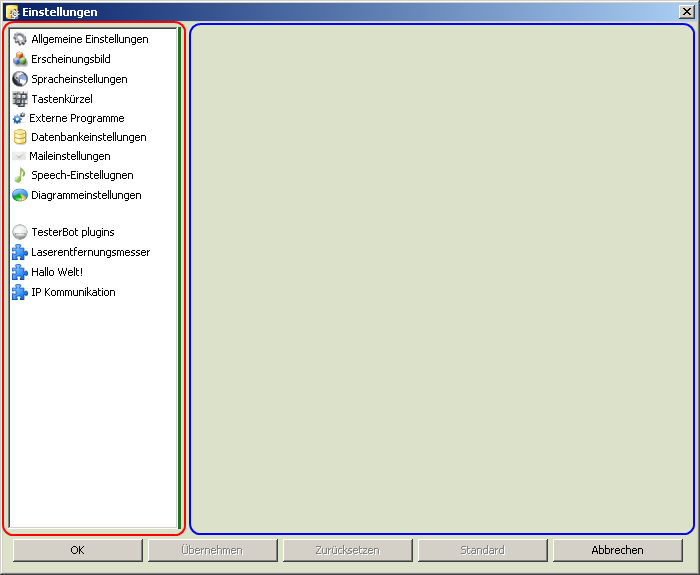
\includegraphics[width=1\textwidth]{images/settingsdialog}
    \caption{Der Settingsdialog mit markierten Kategorie- und Inhaltsbereichen}
    \label{img:settings:dialog}
\end{figure}

Um die Einstellungen einer Kategorie oder eines Plugins vorzunehmen, muss durch
einen Klick auf das entsprechende Listenelement auf der linken Seite der Inhalt
aufgerufen werden. In der Abbildung \ref{img:settings:content}
auf Seite \pageref{img:settings:content} ist der Inhalt f�r
\enquote{Allgemeinen Einstellungen} zu sehen.

\begin{figure}[hp]
    \centering
    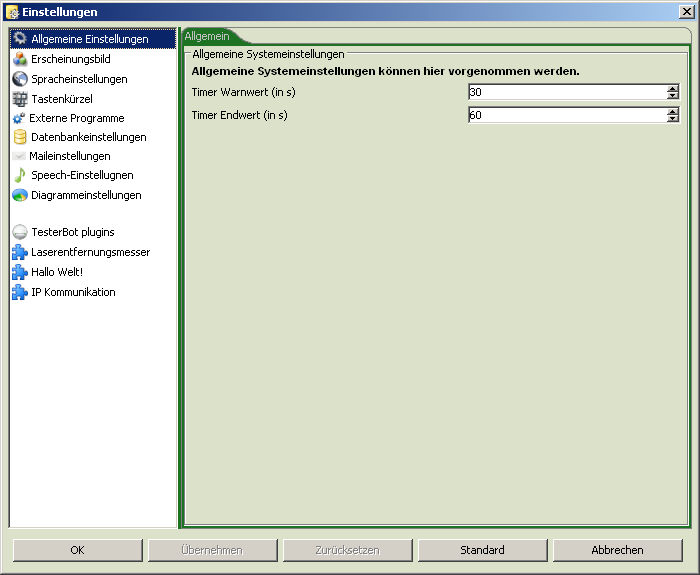
\includegraphics[width=1\textwidth]{images/settingscontent}
    \caption{Der Settingsdialog mit ge�ffnetem \enquote{Allgemeine Einstellungen}
    Inhalt}
    \label{img:settings:content}
\end{figure}

\newpage

Wie in den Abbildungen zu sehen gibt es diverse Kn�pfe die man anklicken k�nnte.

\begin{itemize}
  \item \texttt{OK}, speichert die neuen Einstellungen und schie�t den Dialog
  \item \texttt{�bernehmen}, speichert die neuen Einstellungen
  \item \texttt{Zur�cksetzen}, setzt auf den zuletzt gespeicherten Wert zur�ck
  \item \texttt{Standard}, setzt den Wert auf seinen Standard Wert
  \item \texttt{Abbrechen}, verwirft alle neuen Einstellungen und schlie�t den Dialog
\end{itemize}

\texttt{Zur�cksetzen} und \texttt{Standard} sind nur verf�gbar, wenn die Funktion
von den Einstellungen unterst�tzt wird.

In den folgenden Abschnitten werden die einzelnen Einstellungsm�glichkeiten der
Anwendung erl�utert.

\section{Allgemeine Einstellungen}
In den allgemeinen Einstellungen gibt es zwei Werte die einstellbar sind.

\begin{itemize}
  \item Timer Warnwert
  \item Timer Endwert
\end{itemize}

Die Werte f�r diese Einstellungen werden in Sekunden angegeben. Sie werden bei
der Farbberechnung der Stoppuhr Anzeige benutzt. Nach den im Warnwert
angegebenen Sekunden wechselt die Anzeige ihre Farbe nach orange. Wird der
Endwert erreicht, wechselt die Anzeige ihre Farbe nach rot.

\section{Erscheinungsbild}
In den Einstellungen f�r das Erscheinungsbild der Anwendung gibt es sieben
Farboptionen.

\begin{itemize}
  \item Reiterfarbe
  \item Reiterschriftfarbe
  \item Textfarbe eines inaktiven Reiters
  \item Farbe f�r diverse Elemente die den Fokus haben
  \item Trennlinienfarbe
  \item Hintergrundfarbe
  \item Farbe der Elementtitel
\end{itemize}

Eine Demonstration der Farbenwerte kann in Abbildung \ref{img:settings:badcolor}
auf Seite \pageref{img:settings:badcolor} betrachtet werden.

\begin{figure}[ht]
    \centering
    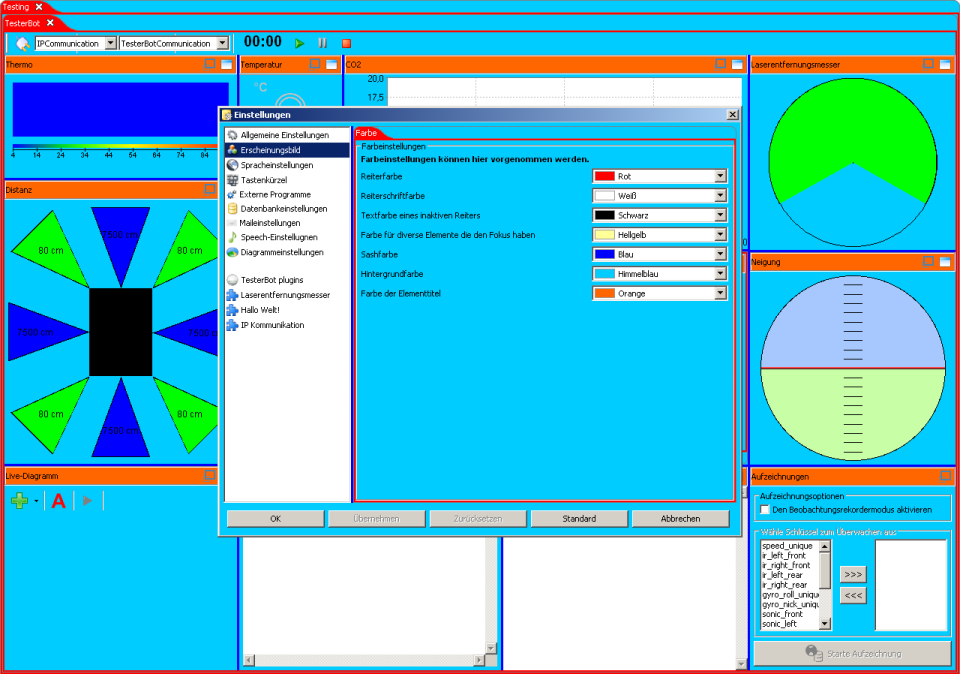
\includegraphics[width=1\textwidth]{images/badcolors}
    \caption{\xirp~mit abweichender Kolorierung zum Verdeutlichung der Farboptionen}
    \label{img:settings:badcolor}
\end{figure}

\section{Spracheinstellungen}
\index{Internationalisierung}
In den Spracheinstellungen gibt es nur eine Option: Die zu verwendende Sprache
der Anwendung. \xirp~unterst�tzt momentan die folgenden Sprachen. Weitere
Sprachpakete sollen in Zukunft folgen.

\begin{itemize}
  \item Deutsch
  \item Englisch
\end{itemize}

Die eingestellte Sprache gilt sowohl f�r die Anwendung als auch f�r die
geladenen Plugins. Sollte ein Plugin f�r die eingestellte Sprache keine
Sprachdatei zur Verf�gung stellen wird die Standard Sprache des Plugins
benutzt.

\section{Tastenk�rzel}
Die Kategorie \enquote{Tastenk�rzel} enth�lt zwei Typen von Tastenk�rzeln.

\begin{itemize}
  \item Anwendungsk�rzel, z.B. Strg+Q
  \item Kommandok�rzel
\end{itemize}

\subsection{Anwendungsk�rzel}
\index{Hotkey}
Die Anwendungsk�rzel werden benutzt um oft benutzte Funktionen mittels einer
Tastenkombination verf�gbar zu machen. In \xirp~gibt es diverse Tastenk�rzel. In
den Einstellungen gibt es eine Aufteilung nach den Tasten vor dem eigentlichen
\seegls{Hotkey}.

\begin{itemize}
  \item Strg+
  \item Strg+Umschalt+
  \item Strg+Alt+
\end{itemize}

F�r jede dieser 3 M�glichkeiten existiert ein eigener Reiter auf der Inhaltsseite
der Einstellungen. Die einzelnen verf�gbaren Funktionen werden im folgenden
erl�utert.

\newpage

\subsubsection{Strg+ - Tastenk�rzel}
\index{Hotkey}
Es existieren sieben Funktionen deren Tastenk�rzel frei bestimmt werden kann.
Der \enquote{\seegls{Hotkey}} wird nach der Steuerung-Taste (Strg) erwartet.

\begin{itemize}
  \item Programm beenden
  \item Einstellungen �ffnen
  \item Hilfe anzeigen
  \item Mailverwaltung �ffnen
  \item Konfigurationsdialog f�r den Diagrammgenerator �ffnen
  \item Reportsuche �ffnen
  \item Kontaktverwaltung �ffnen
\end{itemize}

\subsubsection{Strg+Umschalt+ - Tastenk�rzel}
\index{Hotkey}
Es existiert eine Funktion deren Tastenk�rzel frei bestimmt werden kann.
Der \enquote{\seegls{Hotkey}} wird nach der Steuerung- plus der Umschalt-Taste
(Strg+Umschalt) erwartet.

\begin{itemize}
  \item Programminformationen anzeigen
\end{itemize}

\subsubsection{Strg+Alt+ - Tastenk�rzel}
Es existiert eine Funktion deren Tastenk�rzel frei bestimmt werden kann.
Der \enquote{\seegls{Hotkey}} wird nach der Steuerung- plus der Alt-Taste
(Strg+Alt) erwartet.

\begin{itemize}
  \item Plugininformationen anzeigen
\end{itemize}

\subsection{Kommando Tastenk�rzel}
\index{Kommandos}
\index{Kommandos!kommandierbar}
\index{Gamepad}
Plugins k�nnen kommandierbar sein, das bedeutet, dass ein Plugin/eine Klasse
gewissen Funktionen f�r Kommandos freigeben kann. Zum Beispiel k�nnte eine
\enquote{Notaus} Funktion freigegeben werden. Um diese Funktion nutzen zu
k�nnen muss f�r die Funktion entweder eine Taste der Tastatur, eine Taste eines
\seegls{Gamepad}s, oder beides hinterlegt werden. Dies kann in dem Inhaltsreiter
\enquote{Kommando Tastenk�rzel} getan werden. Die dort vorhandene Tabelle
enth�lt alle verf�gbaren Kommando-Funktionen (Siehe Abbildung
\ref{img:settings:commads} auf Seite \pageref{img:settings:commads}).

\begin{figure}[hbp]
    \centering
    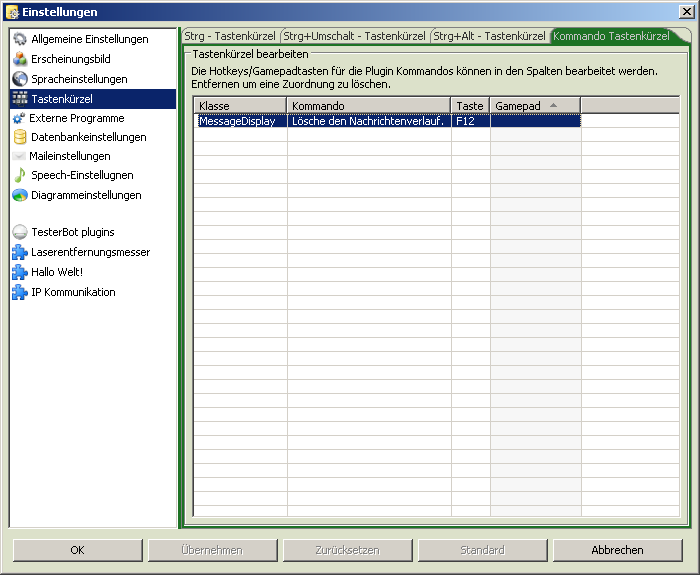
\includegraphics[width=1\textwidth]{images/commands}
    \caption{Kommando Tastenk�rzel Konfiguration}
    \label{img:settings:commads}
\end{figure}

Wie zu sehen ist, wurde der Funktion \enquote{L�sche den Nachrichtenverlauf.}
der Klasse \enquote{MessageDisplay} die Tastaturtaste \enquote{F12} zugewiesen.
Eine Gamepadtaste wurde noch nicht zugewiesen. Um nun die Taste zu �ndern oder
hinzuzuf�gen muss nur auf die entsprechende Tabellenzelle geklickt werden. Hier
�ffnet sich nun ein Eingabefeld. Dann muss nur noch die gew�nschte
Tastatur-/Gamepadtaste gedr�ckt werden.

\section{Externe Werkzeuge}
\index{Externe Werkzeuge}
In den Einstellungen f�r die externen Programme der \seegls{Profile} gibt es pro
geladenem Profil einen Inhaltsreiter. Jeder dieser Reiter enth�lt die
Konfigurationsoberfl�che die in Abbildung \ref{img:settings:ext} auf Seite
\pageref{img:settings:ext} zu sehen ist.

\begin{figure}[hp]
    \centering
    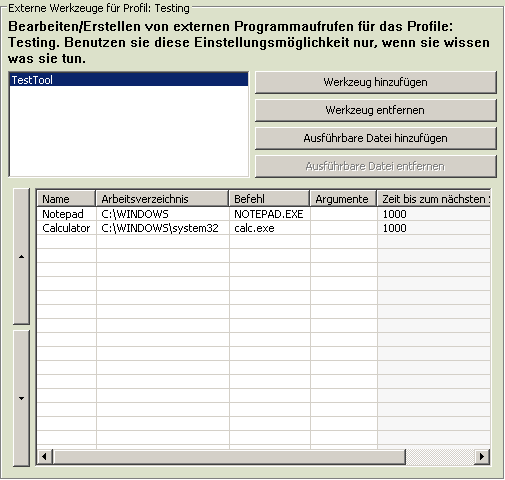
\includegraphics[width=.75\textwidth]{images/ext}
    \caption{Oberfl�che zum konfigurieren der externen Programme}
    \label{img:settings:ext}
\end{figure}

Um ein neues externes Werkzeug anzulegen muss einfach auf den Knopf
\enquote{Werkzeug hinzuf�gen} geklickt werden. Dann muss in dem folgenden
Eingabedialog der Name des Werkzeugs angegeben werden. Ist dies erfolgreich
wird in der List das neue Werkzeug angezeigt. Der n�chste Schritt ist nun diesem
Werkzeug mindestens ein ausf�hrbares Programm zuzuordnen. Dazu muss zuerst das
Werkzeug in der Liste markiert werden und dann auf den Knopf
\enquote{Ausf�hrbare Datei hinzuf�gen} geklickt werden.
\par
Der folgende Eingabedialog erwartet zwei Pflichtangaben: Den Namen des Programms
und die Wartezeit nach Start der Anwendung. Der Name des Programms ist frei
w�hlbar. In dem Beispiel in Abbildung \ref{img:settings:ext:example} auf Seite
\pageref{img:settings:ext:example} ist als Name \enquote{Firefox} gew�hlt. Die
Wartezeit nach dem Start wird in Millisekunden angegeben. Dieser Wert kann
genutzt werden, um einem Programm eine gewissen zeitlichen Spielraum zu
verschaffen, bis ein weiteres gestartet wird. Dies ist n�tzlich falls
nachfolgende Programme von vorherigen abh�ngig sind.

\begin{figure}[hp]
    \centering
    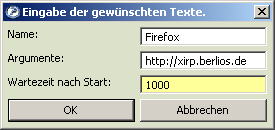
\includegraphics[width=0.5\textwidth]{images/ext_example}
    \caption{Beispieleingabe f�r ein ausf�hrbares Programm}
    \label{img:settings:ext:example}
\end{figure}

Die \enquote{Argumente} Eingabe ist optional. Hier k�nnen Argumente angegeben
werden die ein Programm beim Start ben�tigt. Wird dieser Eingabedialog best�tigt
erscheint ein Dateiauswahldialog. Erst jetzt wird die eigentliche ausf�hrbare
Datei ausgew�hlt.
\par
Wurden zu einem Werkzeug mehrere Programme hinzugef�gt kann die Reihenfolge in
der sie gestartet werden sollen mittels der Pfeiltasten auf der linken Seiten
ver�ndert werden.

\section{Datenbankeinstellungen}
\index{Datenbank}
In den Einstellungen f�r die Datenbank gibt es f�nf Optionen die eingestellt
werden k�nnen.

\begin{itemize}
  \item IP-Adresse
  \item Port
  \item Benutzer
  \item Passwort
  \item Datenbanktreiber
\end{itemize}

\newpage

Die ersten vier Optionen beziehen sich auf Datenbanken die �ber \seegls{TCP/IP}
kommunizieren. Diese sollten angegeben werden, wenn ein Datenbanktreiber gew�hlt
wird der diese Einstellungen ben�tigt. Momentan werden die folgenden Datenbanken
unterst�tzt.

\begin{itemize}
  \item HSQLDB
  \item MySQL
\end{itemize}

\index{Rekorder}
\index{Reporte}
Die \enquote{HSQSLDB} wird bei der Installation von \xirp~mitgeliefert, so dass
kein spezieller Datenbankserver vorhanden sein muss, um Aufzeichnungen mit dem
Rekorder vorzunehmen und Reporte abzuspeichern.

\section{Maileinstellungen}
\index{Mail}
In den Einstellungen f�r das Mailsystem gibt es sechs Optionen die eingestellt
werden k�nnen.

\begin{itemize}
  \item SMTP-Host
  \item Port
  \item Authentifizierung n�tig
  \item Benutzername
  \item Passwort
  \item No-Reply Adresse
\end{itemize}

Hier k�nnen die f�r die Kommunikation mit dem SMTP-\seegls{Server} n�tigen Einstellungen
gemacht werden. Die \enquote{No-Reply} Adresse muss gesetzt werden, da sonst das
Versenden von E-Mails nicht funktionieren wird.

\section{Speech-Einstellungen}
\index{Text-To-Speech}
\index{Sprachausgabe}
In den Einstellungen f�r das Speech-System\footnote{Bisher wird nur
Sprachausgabe unterst�tzt. Spracherkennung soll in einer zuk�nftigen Version
hinzukommen} gibt es zwei Optionen die eingestellt werden k�nnen.

\begin{itemize}
  \item Stimme der Sprachausgabe
  \item Sprachausgabe aktivieren
\end{itemize}

Die erste Option bestimmt die Stimme die f�r die Sprachausgabe benutzt werden
soll. Es gibt zwei Standard Sprachen:

\begin{itemize}
  \item kevin
  \item kevin16
\end{itemize}

Das Sprachausgabesystem unterst�tzt \enquote{MBROLA} Stimmen. Wenn diese
installiert werden, werden die neu hinzugekommenen Stimmen ebenfalls hier zur
Auswahl gestellt. in Kapitel \ref{ref:speech} ab Seite \pageref{ref:speech} kann
nachgelesen werden, wie diese zus�tzlichen Stimmen installiert werden k�nnen und
woher man diese beziehen kann.

\section{Diagrammeinstellungen}
\label{ref:settings:livechart}
\index{Live-Diagramme}
\index{Live-Diagramme!PDF}
\index{Live-Diagramme!PNG}
\index{Live-Diagramme!JPG}
\index{Live-Diagramme!CSV}
In den Einstellungen f�r die Live-Diagramme gibt es vier Optionen die eingestellt
werden k�nnen. Alle beziehen sich darauf, ob nach dem Stoppen eines
Plottingvorgangs das erzeugte Diagramm in verschiedenen Formaten automatisch
exportiert werden sollen.

\begin{itemize}
  \item PDF beim Stoppen eines Live-Diagramms automatisch exportieren
  \item PNG beim Stoppen eines Live-Diagramms automatisch exportieren
  \item JPG beim Stoppen eines Live-Diagramms automatisch exportieren
  \item CSV beim Stoppen eines Live-Diagramms automatisch exportieren
\end{itemize}

\index{Einstellungen|)}

\chapter{Report}
\label{sec:report}
\index{Report}

\xirp~erm�glicht es dem \seegls{Plugin}-Entwickler eine Reportdatenstruktur zu benutzen,
um einen \seegls{PDF}-Report erstellen zu lassen. Ein Beispiel, wie ein solcher Report in
ein \seegls{Plugin} eingebaut werden kann bindet sich unter \autoref{sec:plugin:report}
auf \autopageref{sec:plugin:report}.
\index{Manager!ReportManager}
In diesem Kapitel wird n�her auf die mit Inhalt zu f�llende Datenstruktur
\texttt{Report} und deren abh�ngige Klassen eingegangen. Danach wird kurz auf den
\texttt{ReportManager} eingegangen.

\newpage

\section{Die Report-Datenstruktur}
Die Report-Datenstruktur ist in Abbildung \autoref{img:report:datastructure}
auf \autopageref{img:report:datastructure} schematisch zu sehen. Es ist
erkennbar, dass die Klasse \texttt{Report} mit einem \texttt{Content},
\texttt{Header} und dem Namens-\texttt{String} komplett gef�llt ist.

\kfig{report-datastructure}{.5}{Eine schematische Darstellung der
Report-Datenstruktur}{img:report:datastructure}

Daher l�sst sich ein \texttt{Report}-Objekt nicht mittels des
Default-Konstruktors erzeugen, sondern nur mit dem in
\autoref{lst:report:constr} auf \autopageref{lst:report:constr}.

\begin{java}[caption=Der zu benutzende Konstruktor f�r Reporte,
label=lst:report:constr]
public Report(Header header, Content content, String name){
	[...]
}
\end{java}

Auf die Erstellung der \texttt{Header} und \texttt{Datenstrukturen} wird in den
folgenden Abschnitten eingegangen.

\section{Die Header-Datenstruktur}
Die Kopfdaten des Reportes werden in der Datenstruktur \texttt{Header}
gesammelt. Um einen Header zu erstellen kann einer der in
\autoref{lst:report:head:constr} auf \autopageref{lst:report:head:constr}
gezeigten Konstruktoren benutzt werden. Der Default-Konstruktor
ist auch hier nicht verf�gbar, da die Kopfinformationen komplett sein m�ssen.

\begin{java}[caption=Die zu benutzenden Konstruktoren f�r Header,
label=lst:report:head:constr]
public Header(String title, Robot robot) {
	[...]
}

public Header(String title, Robot robot, IPlugable plugin) {
	[...]
}
\end{java}

Es muss also mindestens der Titel des Reportes und der Roboter f�r den der
Report erstellt wird angegeben werden. Als Zusatzinformation kann noch das
Erstellende \seegls{Plugin}\index{Plugin} angegeben werden.

\section{Die Content-Datenstruktur}
Der Inhalt des Reportes wird in der Datenstruktur \texttt{Content} gesammelt.
Ein \texttt{Content}-Objekt kann mittels des Default-Konstruktors erstellt
werden. Die Inhaltsteile werden dann nach und nach hinzugef�gt. Um einen
Inhaltsteil zum Inhalt hinzuzuf�gen kann die Methode
\codeQuote{addReportPart(ContentPart)} benutzt werden.

\subsection{Die ContentPart-Datenstruktur}
Einem \texttt{ContentPart} k�nnen \texttt{IContentPartItem}-Objekte hinzugef�gt
werden. Momentan gibt es f�nf Implementierungen des
\texttt{IContentPartItem}-Interfaces. 

\begin{itemize}
  \item \texttt{ContentPartImage} - Ein Bild im Report.
  \item \texttt{ContentPartList} - Eine Aufz�hlung im Report.
  \item \texttt{ContentPartTable} - Eine Tabelle im Report.
  \item \texttt{ContentPartText} - Ein Text im Report.
  \item \texttt{ContentPartVideo}\footnote{Das Hinzuf�gen wird momentan noch
  nicht unterst�tzt.} - Ein Video im \seegls{PDF}.
\end{itemize}

Um die \texttt{IContentPartItem}-Objekte hinzuzuf�gen gibt es f�nf
korrespondierende und eine allgemeine Methode.

\begin{itemize}
  \item \codeQuote{addReportImage(ContentPartImage)}
  \item \codeQuote{addReportList(ContentPartList)}
  \item \codeQuote{addReportTable(ContentPartTable)}
  \item \codeQuote{addReportText(ContentPartText)}
  \item \codeQuote{addReportVideo(ContentPartVideo)}\footnote{Die Methode f�gt
  momentan das Item nicht hinzu, da das Einbetten von Video noch nicht
  unterst�tzt ist. Dies soll ab Version 3.0.0 m�glich sein.}
  \item \codeQuote{addReportItem(IContentPartItem)}
\end{itemize}

\subsubsection{Die ContentPartImage-Datenstruktur}
Ein Objekt der \texttt{ContentPartImage}-Datenstruktur kann ebenfalls nur
mittels eines speziellen Konstruktors erstellt werden, um zerst�rte Bildeintr�ge
zu minimieren. Um ein Objekt zu erstellen kann der Konstruktor aus 
\autoref{lst:report:content:image:constr} auf
\autopageref{lst:report:content:image:constr} benutzt werden.

\begin{java}[caption=Der zu benutzende Konstruktor f�r ein Bild im Inhalt,
label=lst:report:content:image:constr]
public ContentPartImage(String path, String shortDescription) {
	[...]
}
\end{java}

\subsubsection{Die ContentPartList-Datenstruktur}
Ein \texttt{ContentPartList}-Objekt kann mittels des Default-Konstruktors
erstellt werden. Danach kann der Listentyp gesetzt werden und Eintr�ge
hinzugef�gt werden. Ein Beispiel hierf�r ist in
\autoref{lst:report:content:list:bsp} auf
\autopageref{lst:report:content:list:bsp} zu sehen. Es gibt drei Listentypen:

\begin{itemize}
  \item \codeQuote{BULLET} - Jeder Eintrag beginnt mit einem Bullet, einem dicken
  Punkt.
  \item \codeQuote{NUMBER} - Eine nummerierte Liste.
  \item \codeQuote{DASH} - Jeder Eintrag beginnt mit einem Spiegelstrich.
\end{itemize}

Der Standard-Listentyp ist eine Liste mit Spiegelstrichen.

\begin{java}[caption=Ein Beispiel f�r eine Liste im Report,
label=lst:report:content:list:bsp]
ContentPartList list = new ContentPartList( );
list.setType(ListType.NUMBER); // Eine nummerierte Liste
list.addEntry(Apfel);
list.addEntry(Orange);
list.addEntry(Pullover);
\end{java}

Da hier durch keinen Konstruktor f�r Vollst�ndigkeit der Liste gesorgt werden
kann, obliegt die Kontrolle hier�ber dem Programmierer.

\subsubsection{Die ContentPartTable-Datenstruktur}
Ein \texttt{ContentPartTable}-Objekt kann mit dem Default-Konstruktor erstellt
werden. Danach m�ssen der Tabellenkopf, die Eintr�ge und eine Kurzbeschreibung
der Tabelle gesetzt werden. Alternativ kann der zweite Kontruktor benutzt
werden, dem diese drei Argumente �bergeben werden m�ssen.

Der Kopf der Tabelle wird in einem \texttt{ContentPartTableHeader}-Objekt
angegeben. Durch die eingegebenen Spalten�berschriften ergibt sich die Anzahl
der Spalten der Tabelle. Wird das Tabelle dann eine Zeile hinzugef�gt, die zu
viele Spalten hat, wird eine \texttt{ReportException} geworfen. Es steht der
Default-Konstruktor und ein weiterer zur Verf�gung. Mit der Methode
\codeQuote{addColumn(String)} kann eine weitere Spalte hinzugef�gt werden. Dem
zweiten Konstruktor kann eine variable Anzahl Strings �bergeben werden, die dann
die Spalten�berschriften darstellen. Trotzdem k�nnen danach weitere Spalten mit
den Methode \codeQuote{addColumn(String)} hinzugef�gt werden.

Ein Tabelleneintrag wird durch Objekte der Klasse \texttt{ContentPartTableRow}
repr�sentiert. Objekte dieser Klassen k�nnen mittels des Default-Konstruktors
oder eines zweiten Kontruktors erstellt werden. Dem zweiten Konstruktor kann ein
String-Array �bergeben werden. Diese Eintrage werden dann der Reihe nach
hinzugef�gt. Wird der Default-Konstruktor benutzt werden die Eintr�ge entweder
mit \codeQuote{addEntry(String)} nach und nach, oder mit
\codeQuote{setEntrys(String[])} alle auf einmal gesetzt.

Beispiele f�r die Tabellenerstellung sind in
\autoref{lst:report:content:tab:bsp} auf
\autopageref{lst:report:content:tab:bsp} zu sehen.

\begin{java}[caption=Ein Beispiel f�r eine Tabelle im Report,
label=lst:report:content:tab:bsp]
// Die Tabelle
ContentPartTable table; 
// Der Tabellenkopf
ContentPartTableHeader header = new ContentPartTableHeader("Eins", "Zwei", "Drei");
// Die Reihen mit dem Inhalt
Vector<ContentPartTableRow> rows = new Vector<ContentPartTableRow>( );

// Ein Reihe
ContentPartTableRow row;		

/* Reihen mit Inahlt f�llen. Darauf achten, dass
 * nicht mehr Felder gef�llt werden, als Spalten zur
 * Verf�gung stehen. Ansonten wird eine ReportExeception
 * geworfen, wenn die Reihen der Tabelle hinzugef�gt werden.
 */
row = new ContentPartTableRow("Inhalt", "Inhalt", "Inhalt");
rows.add(row);

row = new ContentPartTableRow("Inhalt", "Inhalt", "Inhalt");
rows.add(row);

row = new ContentPartTableRow("Inhalt", "Inhalt", "Inhalt");
rows.add(row);

row = new ContentPartTableRow("Inhalt", "Inhalt", "Inhalt");
rows.add(row);

// Tabelle mit den gesammelten Daten erstellen.
try {
	table = new ContentPartTable(header, rows, "Beschreibung");
}
catch (ReportException e) {
	e.printStackTrace( );
}
\end{java}

Da hier durch keinen Konstruktor f�r Vollst�ndigkeit der Tabelle gesorgt werden
kann, obliegt die Kontrolle hier�ber dem Programmierer.

\subsubsection{Die ContentPartText-Datenstruktur}
Ein Textteil eines Reports kann aus mehreren Abschnitten bestehen. Daher k�nnen
einem \texttt{ContentPartText}-Objekt beliebig viele
\texttt{ContentPartTextParagraph}-Objekte hinzugef�gt werden. Die Reihenfolge
in der diese hinzugef�gt werden entspricht nach der Erzeugung des Reports der
Reihenfolge im Dokument. Ein \texttt{ContentPartTextParagraph}-Objekt kann
mittels seines Default-Konstruktors erstellt werden. Dann kann der Text und eine
optionale �berschrift gesetzt werden. Die Erstellung eines
\texttt{ContentPartText}-Objektes mit zwei Abschnitten ist in
\autoref{lst:report:content:text:bsp} auf 
\autopageref{lst:report:content:text:bsp} zu sehen.

\begin{java}[caption=Ein Beispiel f�r Textabschnitte im Report,
label=lst:report:content:text:bsp]
ContentPartText text = new ContentPartText( ); // Der Textteil
ContentPartTextParagraph para; // Ein Abschnittsobjekt
/* [...]: Ein sinnvoller Text */
String foo = "[...]";
String bar = "[...]";

// 1. Abschnitt mit �berschrift
para = new ContentPartTextParagraph( );
para.setHeader("�berschrift");
para.setText(foo);
text.addParagraph(para); // Abschnitt hinzuf�gen

// 2. Abschnitt ohne �berschrift
para = new ContentPartTextParagraph( );
para.setText(bar);
text.addParagraph(para); // Abschnitt hinzuf�gen
\end{java}

Da hier durch keinen Konstruktor f�r Vollst�ndigkeit des Textes gesorgt werden
kann, obliegt die Kontrolle hier�ber dem Programmierer.

\subsubsection{Die ContentPartVideo-Datenstruktur}
Ab Version 3.0.0 soll es m�glich sein auch Videos in das \seegls{PDF} Dokument
einzubetten. Momentan jedoch ist diese Funktionalit�t nicht implementiert.

\section{Der Reportmanager}
\index{Manager!ReportManager}
Mittels des Reportmanagers kann ein \seegls{PDF} zum Betrachten ge�ffnet\footnote{Weitere
Funktionen folgen evtl. in sp�teren Versionen.} werden. Hierzu kann die
statische Methode \codeQuote{viewReport(ReportDescriptor)} aufgerufen werden.
Ein \newline\texttt{ReportDescriptor} kann mittels des Default-Konstruktors erstellt
werden. Dann muss das \texttt{byte[]} des \seegls{PDF}-Dokumentes gesetzt werden, da die
Daten ben�tigt werden, um das \seegls{PDF} zu �ffen. Hierzu k�nnen die Daten nicht direkt
sondern �ber den Dateinamen der \seegls{PDF}-Datei gesetzt werden. Hierzu muss die
Methode \codeQuote{setFileName(String)} aufgerufen werden. Es muss der Dateiname
des generiertes Reports �bergeben werden. Es darf \emph{kein} Pfad vorhanden
sein, denn dieser ist durch die zentrale Speicherung bekannt. Sollte z.B. die
Datei nicht mehr vorhanden sein, wird ein leeres \texttt{byte[]} als Inhalt
erstellt, was dann zu einem Fehler beim �ffnen der Datei f�hrt.

\chapter{Testerbot}
\index{Testerbot|(}

Dieses Kapitel befasst sich mit dem in \xirp~vorhandenen \seegls{Testerbot} \seegls{Server}.
Dieser \seegls{Server} erzeugt f�r verschiedenste \seegls{Sensor}en Zufallswerte und sendet sie an
den verbundenen \seegls{Client}. Dadurch ist es m�glich neue Plugins zu Testen. Der
\seegls{Testerbot} kann auch dazu verwendet werden, die Anwendung zu demonstieren, ohne
dass eine aufw�ndige Roboter-Simulation oder ein echter Roboter benutzt werden m�ssen.

\newpage

\section{Kontrolloberfl�che}
\index{Testerbot!Kontrolloberfl�che}
Der \seegls{Testerbot} \seegls{Server} kann bequem aus der Anwendung heraus gestartet werden. �ber
den Men�eintrag \texttt{Extras --> Testerbot ausf�hren} wird die
Kontrolloberfl�che aufgerufen. Diese Oberfl�che ist in Abbildung
\ref{img:testerbot:control:off} auf Seite \pageref{img:testerbot:control:off} zu
sehen.

\begin{figure}[ht]
    \centering
    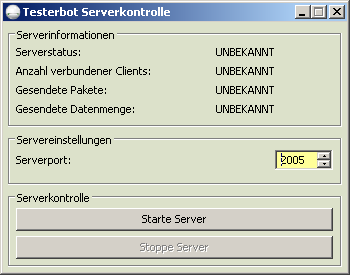
\includegraphics[width=.75\textwidth]{images/tbserverctrl}
    \caption{Die Testerbot Kontrolloberfl�che - Server abgeschaltet.}
    \label{img:testerbot:control:off}
\end{figure}

Die Kontrolloberfl�che ist in drei Bereiche aufgeteilt.

\begin{itemize}
  \item Serverinformationen
  \item Servereinstellungen
  \item Serverkontrolle
\end{itemize}

Die einzelnen Bereiche werden in den folgenden Abschnitten genauer beschrieben.
In Abbildung \ref{img:testerbot:control:on} auf Seite
\pageref{img:testerbot:control:on} ist die Oberfl�che mit aktiviertem \seegls{Server} zu
sehen.

\begin{figure}[ht]
    \centering
    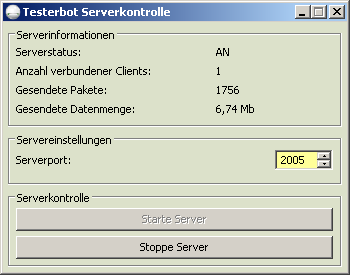
\includegraphics[width=.75\textwidth]{images/tbserverctrl_an}
    \caption{Die Testerbot Kontrolloberfl�che - Server angeschaltet.}
    \label{img:testerbot:control:on}
\end{figure}

\newpage

\subsection{Serverinformationen}
\index{Testerbot!Kontrolloberfl�che!Serverinformationen}
In diesem Bereich werden die folgenden Informationen �ber den \seegls{Server} angezeigt.

\begin{itemize}
  \item Serverstatus (An oder Aus)
  \item Anzahl verbundener Clients
  \item Gesendete Pakete
  \item Gesendete Datenmenge
\end{itemize}

\subsection{Servereinstellungen}
\index{Testerbot!Kontrolloberfl�che!Servereinstellungen}
Die einzige Einstellung die in der Oberfl�che gemacht werden kann ist die
Einstellung des Serverports. Der Standardwert ist \texttt{2005}. Ein neuer Wert
wird bei einem Neustart des \seegls{Server} benutzt.

\subsection{Serverkontrolle}
\index{Testerbot!Kontrolloberfl�che!Serverkontrolle}
In diesen Bereich gibt es zwei Kn�pfe. Nur jeweils einer ist aktiv. Die
Bezeichnung der Kn�pfe spricht f�r sich selbst und seine Funktion.

\begin{itemize}
  \item Starte Server
  \item Stoppe Server
\end{itemize}

Wird die Kontrolloberfl�che geschlossen, wird auch automatisch der \seegls{Server}
beendet. Daher muss die Oberfl�che immer angezeigt werden, wenn der \seegls{Server}
laufen soll. Die Oberfl�che kann allerdings minimiert werden.

\section{Gesendete Werte}
Der \seegls{Server} sendet Werte f�r diverse \seegls{Sensor}en. Die unterst�tzten \seegls{Sensor}en werden
im folgenden beschrieben.

\subsection{Energiequelle}
Es werden Werte f�r zwei Energiequellen gesendet.

\subsection{Infrarot}
Es werden Werte f�r vier Infrarotabstandssensoren gesendet.

\subsection{Ultraschall}
Es werden Werte f�r vier Untraschallabstandssensoren geliefert.

\subsection{Temperatur}
Es wird ein Temperaturwert gesendet.

\subsection{Thermopile}
\index{Live-Diagramm}
\index{Aufzeichungen}
Es wird ein Termopile-Array Scan geliefert. Dieser Scan besteht aus 32 mal 8
Werten. Daher ist dieser \seegls{Sensor} nicht f�r Aufzeichungen und Live-Diagramm
verwendbar.

\subsection{CO$_2$}
Es wird ein Kohlendioxidwert geliefert.

\subsection{Kompass}
Es wird ein Himmelsrichtungswert gesendet.

\subsection{Geschwindigkeit}
Es wird ein Geschwindigkeitswert gesendet.

\subsection{Neigung}
Es werden zwei Werte f�r die horizontale und vertikale Neigung geliefert.

\subsection{Laserscanner}
\index{Live-Diagramm}
\index{Aufzeichungen}
Es wird ein \seegls{Laserscanner} Scan geliefert. Dieser Scan besteht aus mehr als 600
einzelnen Werten, so dass dieser \seegls{Sensor} nicht f�r Aufzeichungen und Live-Diagramm
verwendbar ist.

\subsection{Nachrichten}
Es werden diverse Zufallstextnachrichten vom \seegls{Server} gesendet. Diese k�nnen z.B.
zum Testen der Sprachausgabe benutzt werden.

\index{Testerbot|)}

\chapter{Diverses}
\label{cha:other}
\index{Diverses}

In diesem Kapitel sollen kurz weitere zur Verf�gung stehende Klassen beschrieben
werden.

\section{Gamepad-Steuerung}
\index{Gamepad}\index{Joystick}
\xirp~bietet die M�glichkeit \seegls{Plugins} �ber ein \seegls{Gamepad} oder einen \seegls{Joystick} zu
steuern. 

Einerseits kann dies �ber \index{Kommando}Kommandos
und \index{Hotkey}\seegls{Hotkeys} (\autoref{sec:plugin:commands},
\autopageref{sec:plugin:commands}) erfolgen.
Andernfalls kann auch die \seegls{Gamepad}-\seegls{API} aus dem Paket
\codeQuote{de.unibremen.rr.xirp.io.gamepad} direkt genutzt werden.

\index{Gamepad!Tasten}\index{Gamepad!Achsen}
Zur Zeit werden dabei 32 Tasten und die Achsen \texttt{POV}, \texttt{X}, 
\texttt{Y},	\texttt{Z},	\texttt{R} und	\texttt{U} unterst�tzt.
\index{Manager!GamepadManager}
Um �ber Tastendr�cke und Achsen�nderungen des \seegls{Gamepad} oder \seegls{Joystick} informiert
zu werden k�nnen beim \codeQuote{GamepadManager} mittels
\codeQuote{addGamepadEventListener(GamepadEventListener)} und
\codeQuote{removeGamepadEventListener(GamepadEventListener)}
\index{Gamepad!Listener} an und abgemeldet werden.

Immer wenn nun eine Taste gedr�ckt/losgelassen wird oder sich die Werte der Achsen �ndern
erh�lt der Listener ein \index{Gamepad!Event}Event. Beim dauerhaften dr�cke
einer Taste werden nicht mehrere Events ausgel�st.

Das \index{Gamepad!Event}\codeQuote{GamepadEvent} bietet dann die Methoden um
die aktuellen Werte des Gamepad abzurufen:
\begin{itemize}
  \item \codeQuote{getValues()}: Gibt die aktuellen Werte zusammen mit den
  zugeh�rigen Achsen zur�ck.
  \item \codeQuote{getValue(AxisType)}: Gibt den aktuellen Wert f�r eine
  bestimmte Achse zur�ck.
  \item \codeQuote{getAxisTypes()}: Gibt allen Achsentypen zur�ck, f�r die Werte
  zur Verf�gung stehen.
  \item \codeQuote{getPressed()}: Gibt die Nummern der gerade gedr�ckten Tasten zur�ck.
\end{itemize}

Bei den Achsen ist normalerweise die Basisposition bei 0.0. Der Wert ist jedoch
nicht immer ganz genau und sollte daher gerundet werden um die Basisposition
herauszufinden. F�r die \enquote{Point of View}-Achse ist 0.0 oben und der Wert
f�r die Basisposition kann mittels \codeQuote{AxisType.POV_ZERO} abgerufen
werden. Ob eine Achse in der Basisposition ist l�sst sich mit
\codeQuote{GamepadControl.isBasePosition(AxisType, float)} pr�fen.

\begin{java}[caption=Gamepad Listener anmelden,label=img:gamepad:listener]
GamepadManager.addGamepadEventListener(new GamepadEventListener( ) {

	@Override
	public void axisChanged(GamepadEvent evt) {
		for (Map.Entry<AxisType, Float> entry : evt.getValues( )
				.entrySet( )) {
			if (GamepadControl.isBasePosition(entry.getKey( ),
					entry.getValue( ))) {
				System.out.println(entry.getKey( ) + ": Nullposition");
			}
			else {
				System.out.println(entry.getKey( ) + ": " +
						entry.getValue( ));
			}
		}

	}

	@Override
	public void buttonPressed(GamepadEvent evt) {
		System.out.println("Pressed: " + evt.getPressed( ));
	}

});
\end{java}


\section{Roboter zeichnen}
\index{Robot!RobotDrawHelper}
Der in \seegls{XML} definierte Roboter (\autoref{sec:robotspecs}, 
\autopageref{sec:robotspecs}) hat \seegls{Sensor}en welche eine bestimmte 
Position am Roboter haben (\autoref{sec:sensorgroup}, 
\autopageref{sec:sensorgroup}). In der Roboter�bersicht (Men� 
\menuQuote{Ansicht/Roboter�bersicht}\index{Men�!Ansicht!Roboter�bersicht}) von \xirp~sind die \seegls{Sensor}en des 
Roboter an ihren korrekten Positionen eingezeichnet. Die Berechnung der 
Positionen f�r dieser 2-Dimensionalen Draufsicht erfolgt mittels des 
\codeQuote{RobotDrawHelper}.

\index{Roboter}
Dem Konstruktor wird der Roboter und der Rand �bergeben in welchem nichts
gezeichnet werden soll. Bei einem Rand von 10 w�rden also oben, unten, links und
rechts 10 Pixel frei bleiben. Dieser Rand kann sp�ter noch mittels
\codeQuote{setSpacing(int)} ver�ndert werden.

Die Gr��e des Bereichs auf dem gezeichnet wird (siehe 
\codeQuote{org.eclipse.swt.widgets. Control.addControlListener(ControlListener 
listener)}), wird dem Objekt dann mittels \codeQuote{resized(Point)} �bergeben. 
Dies f�hrt zu einer Neuberechnung des einzeichenbaren Roboterrechtecks welches 
mit \codeQuote{getRobotDrawRectangle()} abgerufen werden kann.

F�r die \seegls{Sensor}en k�nnen die Positionen am Roboterrechteck durch Aufrufe von
\newline\codeQuote{getSensorLocation(Sensor)} berechnet werden.
\index{Manager!ColorManager}
\begin{java}[caption=Roboter mit 2 Sensoren zeichnen,label=code:robotdrawhelper]
private void drawRobot(final Composite comp) throws RobotNotFoundException {
	// Roboter holen
	Robot robot = ProfileManager.getRobot(plugin.getRobotName( ));

	// Sensoren holen
	final Sensorgroup sensorgroup = robot.getSensorgroups( ).get(0);
	final Sensor sensor = sensorgroup.getSensors( ).get(0);

	final Sensorgroup sensorgroup2 = robot.getSensorgroup("Infrared");
	final Sensor sensor2 = sensorgroup2.getSensors( ).get(0);

	// 10 Pixel Rand
	final RobotDrawHelper robotDraw = new RobotDrawHelper(10, robot);

	comp.addControlListener(new ControlAdapter( ) {

		@Override
		public void controlResized(ControlEvent evt) {
			// Danach wird automatisch repaint aufgerufen
			robotDraw.resized(comp.getSize( ));
		}

	});

	comp.addPaintListener(new PaintListener( ) {

		@Override
		public void paintControl(PaintEvent evt) {
			GC gc = evt.gc;
			// Roboter einzeichnen
			gc.setBackground(ColorManager.getColor(SWT.COLOR_RED));
			gc.fillRectangle(robotDraw.getRobotDrawRectangle( ));

			// Sensoren einzeichnen
			gc.setBackground(ColorManager.getColor(SWT.COLOR_BLUE));
			final Point sensorLocation = robotDraw.getSensorLocation(sensor);
			gc.fillOval(sensorLocation.x - 5, sensorLocation.y - 5, 10, 10);
			gc.drawString(sensorgroup.getLongName( ),
					sensorLocation.x + 5,
					sensorLocation.y + 5,
					true);

			final Point sensorLocation2 = robotDraw.getSensorLocation(sensor2);
			gc.fillOval(sensorLocation2.x - 5,
					sensorLocation2.y - 5,
					10,
					10);
			gc.drawString(sensorgroup2.getLongName( ),
					sensorLocation2.x + 5,
					sensorLocation2.y + 5,
					true);
		}

	});

}
\end{java}

\section{Farbverlauf berechnen}
\index{Farbe!Farbverlauf}
Die Klasse \codeQuote{GradientUtil} bietet Zugriff auf Einzelne Bereiche eines
Farbverlaufs. 

Erstellt man zum Beispiel einen Farbverlauf von Rot �ber Gr�n nach Blau und
m�chte wissen welche Farbe bei 75\% des Farbverlaufs gerade aktuell ist, so
l�sst sich dies wie folgt umsetzen:
\begin{java}[caption=Farbverlauf berechnen,label=code:farbverlauf]
GradientUtil gradient = new GradientUtil(new Color[] {Color.RED,
		Color.GREEN, Color.BLUE});
Color color = gradient.getColor(0.75f);
System.out.println("Gleichverteilt bei 75%: " + color);

gradient = new GradientUtil(new float[] {0.0f, 0.5f, 1.0f},
		new Color[] {Color.RED, Color.GREEN, Color.BLUE});
color = gradient.getColor(0.75f);
System.out.println("Mehr Rot bei 75%: " + color);
\end{java}

Ausgabe:
\begin{lstlisting}
Gleichverteilt bei 75%: java.awt.Color[r=0,g=95,b=160]
Mehr Rot bei 75%: java.awt.Color[r=0,g=128,b=127]
\end{lstlisting}

Dieses Beispiel erstellt zum einen einen Farbverlauf mit gleichgro�en
Farbabschnitten f�r die drei Farben und dann eine Farbverlauf der einen gr��eren
Rot-Anteil gegeben�ber dem Gr�nen und Blauen hat.

Die Klasse arbeitet mit \seegls{AWT}-Farben. Zur Umrechnung von \seegls{SWT} in \seegls{AWT} Farben und
zur�ck kann der \index{Manager!ColorManager}\codeQuote{ColorManager} benutzt
werden. 

Diese Klasse soll nicht zum Zeichnen des Farbverlaufs benutzt werden sondern nur
zur Berechnung einzelner Farben im Farbverlauf.

\section{Nachrichten als Tooltip}
\kfig{diverses_ballonwindow}{.5}{BalloonWindow in der
Systemtray}{img:diverses:balloonwindow} 
\xirp~bietet eine M�glichkeit kleine Nachrichten als so genanntes \enquote{Balloon Window}
(eine Art \index{Tooltip}Tooltip) an der \index{Systemtray}\seegls{Systemtray} anzuzeigen
(siehe \autoref{img:diverses:balloonwindow}). Dazu wird die Methode
\codeQuote{showToolTip()} des \index{Manager!MessageManager} 
\codeQuote{MessageManager} benutzt:
\begin{java}[caption=BalloonWindow mit MessageManager erstellen,label=code:messagemanager]
MessageManager.showToolTip("Ein Tooltip",
		"Hier kann eine sch�ne Nachricht stehen",
		MessageType.INFO);
\end{java}


\section{Sprachausgabe}
\index{Sprachausgabe}
\xirp~bietet die M�glichkeit Text in Sprache umzuwandeln und ausgeben zu lassen.
\index{Manager!TextToSpeechManager}
Dazu kann der \codeQuote{TextToSpeechManager} genutzt werden. Dieser bietet die
Methode \codeQuote{speakText()} welche den �bergebenen Text vorliest:
\begin{java}
TextToSpeechManager.speak("Hello World!");
\end{java}

Dazu muss in den \index{Einstellungen}Einstellungen unter \enquote{Speech-Einstellungen} die
Sprachausgabe angeschaltet werden. Mehr Informationen dazu finden sich im
\index{Benutzerhandbuch}Benutzerhandbuch.

\section{Instanziierung}
\index{Instanziierung}
Mit der Klasse \codeQuote{InstanceUtil} lassen sich zum Beispiel Instanzen von
zur Zeit der Kompilierung unbekannten Klassen erstellen.

Als Beispiel wird hier jedoch nur eine Instanz von \codeQuote{GradientUtil}
erstellt:
\begin{java}[caption=Instanz mit InstanceUtil erstellen,label=code:instanceutil]
// Array von Farben f�r GradientUtil
final Color[] colors = new Color[] {Color.RED, Color.GREEN, Color.BLUE};
//Array mit den Prozenten f�r die Farben
float[] percents = new float[] {0.0f, 0.5f, 1.0f};
//Array mit den beiden Argumenten f�r GradientUtil
final Object[] objects = new Object[] {percents, colors};
//Instanz erstellen und benutzen
Object obj = InstanceUtil.createInstance(GradientUtil.class.getName( ),
		objects);
System.out.println(obj);
if (obj != null && obj instanceof GradientUtil) {
	GradientUtil util = (GradientUtil) obj;
	System.out.println(util.getColor(.5f));
}
\end{java}

Die Methode \codeQuote{createInstance(String, Object...)} erh�lt als erstes den
kompletten Klassenname (mit Paket) und dann ein Array von Argumenten welche als
Parameter f�r den Konstruktor benutzt werden. Dabei ist darauf zu achten dass
die gegebenen Argumente exakt den Typ haben muss der vom Konstruktor erwartet
wird. Ist der erwartete Typ \codeQuote{Control} so kann nicht
\codeQuote{Composite} �bergeben werden.

\section{Util}
\index{Util}
In der Klasse \codeQuote{Util} finden sich einige Methoden die w�hrend der
Entwicklung von \xirp~entstanden sind.

\begin{itemize}
  \item \codeQuote{getTimeAsString(Date)}: Formatiert das gegebene Datum im
  Format \enquote{yyyy-MM-dd\_HH-mm-ss}.
  \item \codeQuote{getTimeAsString(Date, String)}: Formatiert das gegebene Datum
  im angegebenen Format.
  \item \codeQuote{getTimeAsString(long)}: Formatiert den f�r ein Datum
  stehenden long \\(\codeQuote{System.currentTimeMillis()}) im Format
  \enquote{yyyy-MM-dd\_HH-mm-ss}.
  \item \codeQuote{getTimeAsString(long, String)}: Formatiert den f�r ein Datum
  stehenden long (\codeQuote{System.currentTimeMillis()}) im angegebenen Format.
  \item \codeQuote{encrypt(String)}: Verschl�sselt den angegebenen String.
  \item \codeQuote{decrypt(String)}: Entschl�sselt einen mit
  \codeQuote{encrypt(String)} verschl�sselten String.
  \item \codeQuote{convertObject(Object, Class<?>)}: Versucht das gegebenen
  Objekt in eines der gegebenen Klasse zu umzuwandeln. Diese Konvertierung
  funktioniert zwischen Zahlenklassen untereinander und immer zu Strings.
  \item \codeQuote{getOptimalMapSize(int)}: Berechnet f�r die gew�nschte Gr��e
  einer \codeQuote{java.util.Map} und ihren normalen Load-Factor die optimale
  Gr��e bei der die \codeQuote{Map} die Elemente ohne ein Rehashing aufnehmen kann.
  \item \codeQuote{isEmpty(String)}: Pr�ft ob der gegebene String
  \codeQuote{null} ist oder nur aus Leerzeichen besteht.
  \item \codeQuote{getEnumNameOrNothing(Enum)}: Gibt f�r das gegebenen
  enum-Element dessen Namen \codeQuote{name()} oder einen leeren String zur�ck
  sofern das Element \codeQuote{null} war.
  \item \codeQuote{scale(double, double, double, double, double)}: Skaliert
  einen Wert aus einem Wertebereich auf einen anderen Wertebereich. Der
  Eingabewertebereich ist dabei durch die ersten, der Ausgabebereich durch die
  n�chsten beiden Parameter gegeben. Die Wert durch den letzten.
  \item \codeQuote{scale(long, long, long, long, long)}: siehe oben.
\end{itemize}

\begin{java}[caption=Die Methoden der Util-Klasse,label=code:util:class]
public static void main(String[] args) {
	System.out.println(Util.getTimeAsString(System.currentTimeMillis( )));
	System.out.println(Util.getTimeAsString(System.currentTimeMillis( ),
			"yyyy"));
	final String encrypt = Util.encrypt("Hallo");
	System.out.println(encrypt);
	System.out.println(Util.decrypt(encrypt));
	System.out.println(Util.convertObject("20", Integer.class));
	System.out.println(Util.getEnumNameOrNothing(Robot.RobotType.WALK));
	System.out.println(Util.scale(100, 200, 0, 100, 150));
}
\end{java}

Die Ausgabe diese Codest�cks w�rde zum Beispiel so aussehen:
\begin{lstlisting}
2007-07-03_23-29-03
2007
aSqVgLgp90U=
Hallo
20
WALK
50
\end{lstlisting}

\section{Versionen vergleichen}
Die Klasse \codeQuote{VersionComparator} bietet die M�glichkeit Versionen
miteinander zu vergleichen oder zu sortieren. Die Versionsnummern d�rfen dabei nur
aus durch Punkte getrennte Zahlen bestehen. Sortiert durch einen Vergleich der
Zahlen zwischen den Punkten. Dabei werden erst alle Zahlen vor dem ersten Punkt,
dann alle vor dem zweiten Punkt und so weiter miteinander verglichen. Buchstaben
folgen immer nach allen Zahlen der selben Ebene:

\begin{java}[caption=Sortierung von Versionsnummern,label=code:versioncomparator]
VersionComparator comp = new VersionComparator( );
List<String> versions = new ArrayList<String>( );
versions.add("1");
versions.add("2.3.1.2");
versions.add("2.a.1.2");
versions.add("1.3.1.2");
versions.add("1.1.1.2");
Collections.sort(versions, comp);
System.out.println(versions);
\end{java}

ergibt folgende Ausgabe:
\begin{lstlisting}
[1, 1.1.1.2, 1.3.1.2, 2.3.1.2, 2.a.1.2]
\end{lstlisting}

\section{Serialisierung}
\index{Serialisierung}
\index{Serialisierung!deep copy}
Um Java Objekte in eine \index{Datei!Java Objekte speicher in}Datei schreiben und
zur�ck lesen zu k�nnen existieren in
\xirp~zwei Klassen die dieses erleichtern sollen. Mit der Methode
\codeQuote{writeToDisk(O, File)} der Klasse \codeQuote{ObjectSerializer} lassen
sich Objekte welche \codeQuote{java.io.Serializable} implementieren in eine
Datei schreiben. Mit der Methode \codeQuote{deepCopy(O)} l�sst sich eine Kopie
eines Objektes erstellen welche keine Verbindung mehr zu dem urspr�nglichen
Objekt hat.

Mit der zweiten Klasse \codeQuote{ObjectDeSerializer} lassen sich �ber die
Methoden \codeQuote{getObject(File)} und \codeQuote{getObject(InputStream)} geschriebene Objekte
wieder aus einen Datei oder von einem Stream einlesen.

\begin{java}[caption=Serialisierung und Deserialisierung,label=code:serial]
public static void main(String[] args) {
	String strg = "Hallo Welt!";
	File f = new File("temp.dat");
	try {
		ObjectSerializer.<String> writeToDisk(strg, f);
		String back = ObjectDeSerializer.<String> getObject(f);
		System.out.println(back);
	}
	catch (IOException e) {
		e.printStackTrace( );
	}
	catch (SerializationException e) {
		e.printStackTrace( );
	}

	int array[] = new int[2];
	array[0] = 5;
	array[1] = 6;

	try {
		int[] copy = ObjectSerializer.<int[]> deepCopy(array);
		copy[1] = 10;

		System.out.println(Arrays.toString(array));
		System.out.println(Arrays.toString(copy));
	}
	catch (IOException e) {
		e.printStackTrace( );
	}
}
\end{java}

Ausgabe:
\begin{lstlisting}
Hallo Welt!
[5, 6]
[5, 10]
\end{lstlisting}

\section{Collections}
\index{Collections}
Bei der Entwicklung von \xirp~reichten die Standard-Collections aus von Java
teilweise nicht aus, so dass einige Erweiterungen dazu entstanden sind.

\subsection{BidiHashMap}
\index{Collections!BidiHashMap}
Bei einer normalen HashMap l�sst sich nur in eine Richtung n�mlich von Schl�ssel
nach einem Wert nachschlagen. Die \codeQuote{BidiHashMap} erm�glicht dies in
zwei Richtungen, wobei dann Schl�ssel und Wert eindeutig sein m�ssen. Es stehen
daher neben den �blichen Methoden einer \codeQuote{HashMap} auch noch folgende
zur Verf�gung:
\begin{itemize}
  \item \codeQuote{removeValue(Object)}: Entfernt den angegebenen Wert und
  seinen Schl�ssel.
  \item \codeQuote{getKey(V)}: Holt den Schl�ssel zum gegebenen Wert.
  \item \codeQuote{keys()}: Gibt eine Liste von Schl�sseln zur�ck.
  \item \codeQuote{valueEntrySet()}: Gibt alle Wert-Schl�ssel-Paare zur�ck.
\end{itemize}

\begin{java}[caption=�bersetzungsdatenbank mit BidiHashMap,label=code:bidihashmap]
public static void main(String[] args) {
	//Kleine �bersetzungsdatenbank
	BidiHashMap<String, String> lookup = new BidiHashMap<String, String>( );
	lookup.put("Hallo", "Hello");
	lookup.put("Welt", "World");
	lookup.put("Guten", "Good");
	lookup.put("Morgen", "Morning");

	//Englische �bersetzung f�r Hallo heraussuchen
	System.out.println(lookup.get("Hallo"));
	//Deutsche �bersetzung f�r Morning raussuchen
	System.out.println(lookup.getKey("Morning"));

	//Alle deutschen �bersetzungen f�r englisch anzeigen
	System.out.println(lookup.valueEntrySet( ));

	//Alle deutschen W�rter anzeigen
	System.out.println(lookup.keys( ));

	//Ein englisches Wort entfernen
	lookup.removeValue("World");

	//Auch das deutsche Wort is weg
	System.out.println(lookup.keys( ));
}
\end{java}
\newpage
Ausgabe:
\begin{lstlisting}
Hello
Morgen
[Morning=Morgen, Good=Guten, World=Welt, Hello=Hallo]
[Morgen, Guten, Welt, Hallo]
[Morgen, Guten, Hallo]
\end{lstlisting}

\subsection{MultiValueHashMap}
\index{Collections!MultiValueHashMap}
In einer normalen \codeQuote{HashMap} l�sst sich f�r jeden Schl�ssel nur ein
Wert ablegen. In der \newline\codeQuote{MultiValueHashMap} werden die Werte dagegen in
einer Liste abgelegt, so dass mehrere Werte f�r einen Schl�ssel erlaubt sind.

Hinzugekommen sind die Methoden \codeQuote{containsValue(K, V)} und
\codeQuote{remove(K, V)} welche pr�fen ob ein Wert \texttt{V} f�r einen
Schl�ssel \texttt{K} vorhanden ist bzw. den Wert von dem Schl�ssel l�scht.

Die Benutzung erfolgt ansonsten wie bei einer normalen \codeQuote{HashMap}, nur
dass beim Abrufen der Werte f�r einen Schl�ssel eine Liste zur�ckgegeben wird.
\begin{java}[caption=Autodatenbank mit einer MultiValueHashMap,label=code:multivaluehashmap]
public static void main(String[] args) {
	MultiValueHashMap<String, String> cars = new MultiValueHashMap<String, String>( );
	cars.put("VW", "Golf");
	cars.put("VW", "Polo");
	cars.put("Peugeot", "206");
	cars.put("Peugeot", "207");
	cars.put("Opel", "Manta");
	cars.put("Opel", "Corsa");

	System.out.println(cars.get("VW"));
	System.out.println(cars.entrySet( ));
}
\end{java}

Ausgabe:
\begin{lstlisting}
[Golf, Polo]
[Peugeot=[206, 207], Opel=[Manta, Corsa], VW=[Golf, Polo]]
\end{lstlisting}

\subsection{ConcurrentMultiValueHashMap}
\index{Collections!ConcurrentMultiValueHashMap}
Die \codeQuote{ConcurrentMultiValueHashMap} ist eine \seegls{Thread}sichere Version der
\codeQuote{MultiValueHashMap} funktioniert aber genau gleich.

\section{L�schen von Dateien}
\index{Datei!l�schen}
\index{Manager!DeleteManager}
\xirp~bietet die M�glichkeit Dateien zur L�schung f�r die Beendigung des
Programms \newline(\codeQuote{deleteOnShutdown()} oder den n�chsten Start
(\codeQuote{deleteOnStartup()} beim
\codeQuote{DeleteManager} einzutragen. K�nnen Dateien bei der  Beendigung
nicht gel�scht werden, zum Beispiel weil sie noch benutzt werden, so werden sie
beim n�chsten Start gel�scht.

\section{Externe Programme starten}
\index{Programm!externes!starten}
\index{Manager!ExternalProgramManager}
Mit dem \codeQuote{ExternalProgramManager} lassen sich Programme starten.

Soll ein im System registriertes Programm gestartet werden um eine Datei zu
�ffnen ist dies eventuelle auch mit \codeQuote{SWTUtil.openFile} m�glich. 

Eigene Programme lassen sich starten indem die Informationen �ber dieses
Programm in ein \codeQuote{ExternalProgram}-Objekt eingetragen werden.

\begin{java}[caption=Externes Programm definieren,label=code:externalprogram]
ExternalProgram program = new ExternalProgram("AcrobatReader",
		"C:/Programme/Adobe/Reader 8.0/Reader",
		"AcroRd32.exe",
		"",
		50);
\end{java}

Das erste Argument ist dabei ein Name f�r das Programm. Dieser kann frei gew�hlt
werden. Das zweite Argument ist der Pfad in welchem das Programm ausgef�hrt
werden soll. Das dritte ist die ausf�hrbare Datei, das f�nfte die Argumente und das
vierte die Zeit in Millisekunden die das Programm ungef�hr zum Starten ben�tigt.

Das Programm wird dann mit dem \codeQuote{ExternalProgramManager} gestartet:
\begin{java}[caption=Starten von 2 externen Programmen,label=code:externalprogrammanager]
ExternalProgram reader = new ExternalProgram("AcrobatReader",
		"C:/Programme/Adobe/Reader 8.0/Reader",
		"AcroRd32.exe",
		"",
		TimeUnit.SECONDS.toMillis(20));
ExternalProgram firefox = new ExternalProgram("Firefox",
		"C:/Programme/Mozilla Firefox",
		"firefox.exe",
		"http://xirp.berlios.de",
		50);

List<ExternalProgram> programs = new ArrayList<ExternalProgram>( );
programs.add(reader);
programs.add(firefox);

ExternalProgramManager.start(programs);
\end{java}
In diesem Beispiel wird zun�chst der Acrobat Reader und dann mit 20 Sekunden
Abstand der Firefox gestartet.

Bei der Beendigung von \xirp~werden alle vom \codeQuote{ExternalProgramManager}
gestarteten Programme beendet sofern sie dies noch nicht sind.

\section{Dateien drucken}
\index{Datei!drucken}
\index{Manager!PrintManager}
Mit dem \codeQuote{PrintManager} lassen sich aus \xirp~heraus auch Dateien
drucken. Dazu muss der \codeQuote{print()}-Methode einfache eine Datei oder eine
Liste von Dateien die gedruckt werden sollen �bergeben werden:

\begin{java}[caption=Eine Datei ausdrucken,label=code:printmanager]
PrintManager.print(new File(Constants.LOG_DIR + Constants.FS +
		"xirp.log"));
\end{java}

% \begin{itemize}
% \item Chart?
% \item Datenbank
% \item Mail?
% \end{itemize}

%\section{Ein erstes Plugin}
\label{sec:firstplugin}
\index{Plugin!erstellen|(}
Voraussetzungen:
\begin{itemize}
\item Java (\seegls{JDK}) ab 1.6
\item Entwicklungsumgebung wie eclipse
\item \xirp~Installation
\end{itemize}

Der erste Schritt ist das erstellen eines neuen Projektes und hinzuf�gen des
\xirp~jar aus dem Installationsordner sowie
des \seegls{SWT} Jar aus dem Unterordner \fileQuote{lib/windows} oder \fileQuote{lib/linux} und hinzuf�gen.

Dann kann eine neue Klasse erstellt werden, welche
\index{Plugin!IPlugable!AbstractPlugin}
\newline\codeQuote{de.unibremen.rr.xirp.plugin.AbstractPlugin} erweitert (\refFig{newPluginClass}). \par
\kfig{plugin_plugin_newPluginClass}{1}{Erstellen einer neuen Pluginklasse}{newPluginClass}

Damit die Applikation wei�, dass diese neu erstellte Klasse die \index{Plugin!Hauptklasse}Hauptklasse 
des Plugins ist, muss eine \index{Plugin!Properties}properties Datei erstellt werden (\refFig{properties}).

Eine Vorlage dieser Properties Datei befindet sich bei der Installation im Ordner 
\fileQuote{development} als \fileQuote{plugin.properties.template}. Diese Datei in das Paket der 
\seegls{Plugin}-Klasse kopieren und die Endung \texttt{.template} entfernen.

\kfig{plugin_properties}{1}{Eine \enquote{plugin.properties}-Datei}{properties}

Nun k�nnen die Methoden mit Inhalten gef�llt werden.

Die Methode \index{Plugin!IPlugable!runInternal()}\codeQuote{runInternal()} 
wird ausgef�hrt wenn das Plugin gestartet wird. Um eine Ausgabe im 
Systemprotokoll von \xirp~zu erhalten muss noch eine Konstante f�r das 
\seegls{Logging} definiert werden.

Dies sieht wie folgt aus:
\codeQuote{private static final RobotLogger LOGGER = RobotLogger.getLogger(MyPlugin.class);}

Der \index{Roboter!Logging}\index{Logging!Roboter}\codeQuote{RobotLogger} ist im Paket 
\codeQuote{de.unibremen.rr.xirp.io.logging} zu finden. 

Die Ausgabe in 
\codeQuote{runInternal()} erfolgt dann �ber 
\codeQuote{LOGGER.info(robotName,''Ausgabe'');}. 

Die Methoden 
\index{Plugin!IPlugable!getPluginType()}\codeQuote{getPluginType()} gibt den 
Typ des Plugins zur�ck. Die \seegls{Plugin} Typen kommen aus der Klasse 
\index{Plugin!PluginType}\codeQuote{de.unibremen.rr.xirp.plugin.PluginType}. �hnliches
gilt f�r den 
\index{Plugin!VisualizationType}Darstellungstyp den die Methoden 
\index{Plugin!IPlugable!getVisualizationType()}\codeQuote{getVisualizationType()} 
zur�ckgibt.

Die Methoden 
\index{Plugin!IPlugable!getDescriptionKey()}\codeQuote{getDescriptionKey()} und 
\index{Plugin!IPlugable!getNameKey()}\codeQuote{getNameKey()} geben einen Schl�ssel 
zur \index{Internationalisierung!Schl�ssel}�bersetzung des \seegls{Plugin} Namens und der \seegls{Plugin} Beschreibung zur�ck.

\kfig{plugin_basicProperties}{1}{�bersetzungsdateien f�r ein Plugin}{basicProperties}

F�r die �bersetzung kommen nun noch zwei weitere Dateien 
(\refFig{basicProperties}) hinzu:\\
\index{Internationalisierung!Plugin}\fileQuote{messages$\_$de.properties} f�r 
die Deutsche �bersetzung und 
\index{Internationalisierung!Plugin}\fileQuote{messages$\_$en.properties} f�r 
die Englische �bersetzung.

Die entstandene Java-Klasse ist in \autoref{stubsFilled} zu sehen.

Das erste \seegls{Plugin} ist nun fast fertig. Nun muss nur noch ein Jar daraus erstellt
werden. Dazu kann aus dem Ordner \fileQuote{development} der Installation die \seegls{Ant}-\fileQuote{build.xml}
in den Hauptordner des Projekts kopiert werden.

Die Pfade oben in der \index{Ant!build.xml}\fileQuote{build.xml} m�ssen entsprechend angepasst werden. Dies 
betrifft normalerweise nur den Eintrag \codeQuote{plugins.pkg}.

Dann kann der Task \index{Ant!build.xml!singlePlugin}\codeQuote{singlePlugin} ausgef�hrt werden. Im Ordner \fileQuote{jar} liegt nun ein 
jar des \seegls{Plugins}. Dieses kann nun in die \xirp~Installation in den Ordner \fileQuote{plugins} 
kopiert werden.

Startet man nun \xirp~wird das \seegls{Plugin} geladen. Ob dies funktioniert hat kann man 
�ber das Men� \menuQuote{?} und den Eintrag \index{Men�!?!�ber Plugins}\menuQuote{�ber Plugins}
herausfinden. Wurde das \seegls{Plugin} 
geladen so ist es dort in der Tabelle aufgelistet (\refFig{aboutPlugins}).

\kfig{plugin_stubsFilled}{1}{Eine einfache Pluginklasse: MyPlugin.java}{stubsFilled}

\kfig{plugin_aboutPlugins}{1}{Men�: �ber Plugins}{aboutPlugins}

Damit das \seegls{Plugin} ausgef�hrt wird, muss es einem Roboter hinzugef�gt werden.

Dazu kann der Roboter \robotQuote{TesterBot} genutzt werden. Die Definition dieses Roboters 
befindet sich in der Installation \index{Profil!Roboter}\fileQuote{conf/profiles/robots/testerbot.bot}.

\newpage
Um das \seegls{Plugin} einzubinden muss einfach nur ein Element zum Element \codeQuote{plugins} ganz 
unten hinzugef�gt werden welches wie folgt aussieht:\index{Profil!Roboter!Plugin}

\begin{xml}[caption=Plugin in Roboterprofil eintragen,label=lst:smplplug:first:xml]
<plugin name="MeinPlugin">
	<class>xirp.plugins.MyPlugin</class>
	<usemultimedia>false</usemultimedia>
</plugin>
\end{xml}

Startet man \xirp~nun wieder kann man den Roboter \robotQuote{TesterBot} ausw�hlen und findet 
im Men� unter \index{Men�!Plugins}\menuQuote{Plugins} das eigene \seegls{Plugin} wieder. Klickt man darauf so wird das 
\index{Plugin!ausf�hren}\seegls{Plugin} ausgef�hrt und es sollte eine entsprechende Ausgabe im \index{Logging!Systemprotokoll}Systemprotokoll 
erscheinen.

\index{Plugin!erstellen|)}


\index{Roboter!TesterBot|see {TesterBot}}
\index{Plugin!Einstellungen|see {Einstellungen}}
\index{Plugin!Internationalisierung|see {Internationalisierung}}
\index{Plugin!Bild|see {Bild}}
\index{Farbe!Manager|see {Manager, ColorManager}}
\index{Schriftart!Manager|see {Manager, FontManager}}
\index{Bild!Manager|see {Manager, ImageManager}}
\index{Profil!Manager|see {Manager, ProfileManager}}
\index{Joystick|see {Gamepad}}
\newpage

\pagenumbering{alph}
\appendix
% \bibliographystyle{alphadin}
% \bibliography{referenzen}
% \newpage
%\begin{multicols}{2}
\printglossary
%\end{multicols}
\newpage
\printindex

\end{document}
